\chapter[Backgrounds to $\Htautau$][Backgrounds to $\Htautau$]{Backgrounds to $\Htautau$}
\label{chap:results}

\begin{quote}
Background estimates in the $\Htautau$ analysis are described.
\end{quote}

\section{$\Ztautau$}
\label{sec:backgrounds-ztautau}

\begin{figure}[tp]
  \centering
  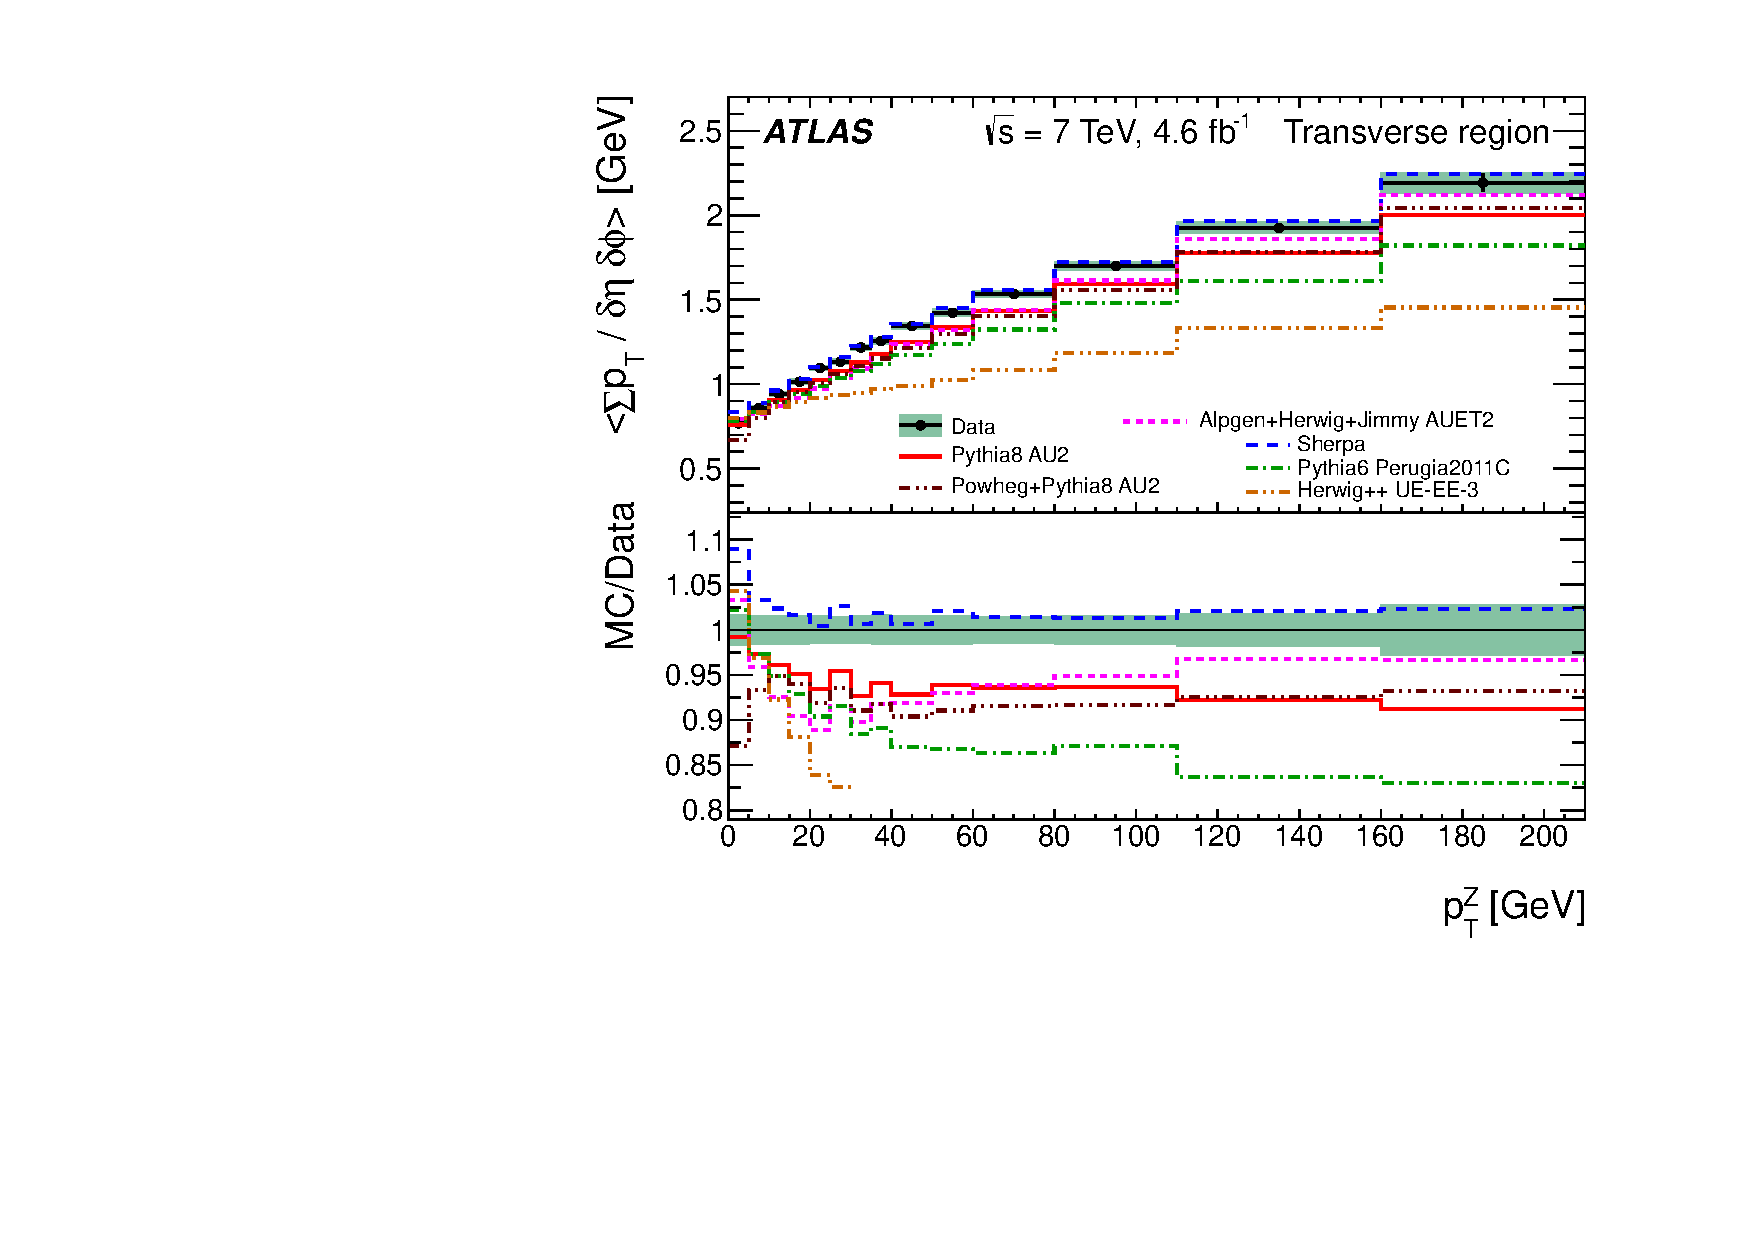
\includegraphics[width=0.48\textwidth]{figures/STDM-2011-42/fig_14b}
  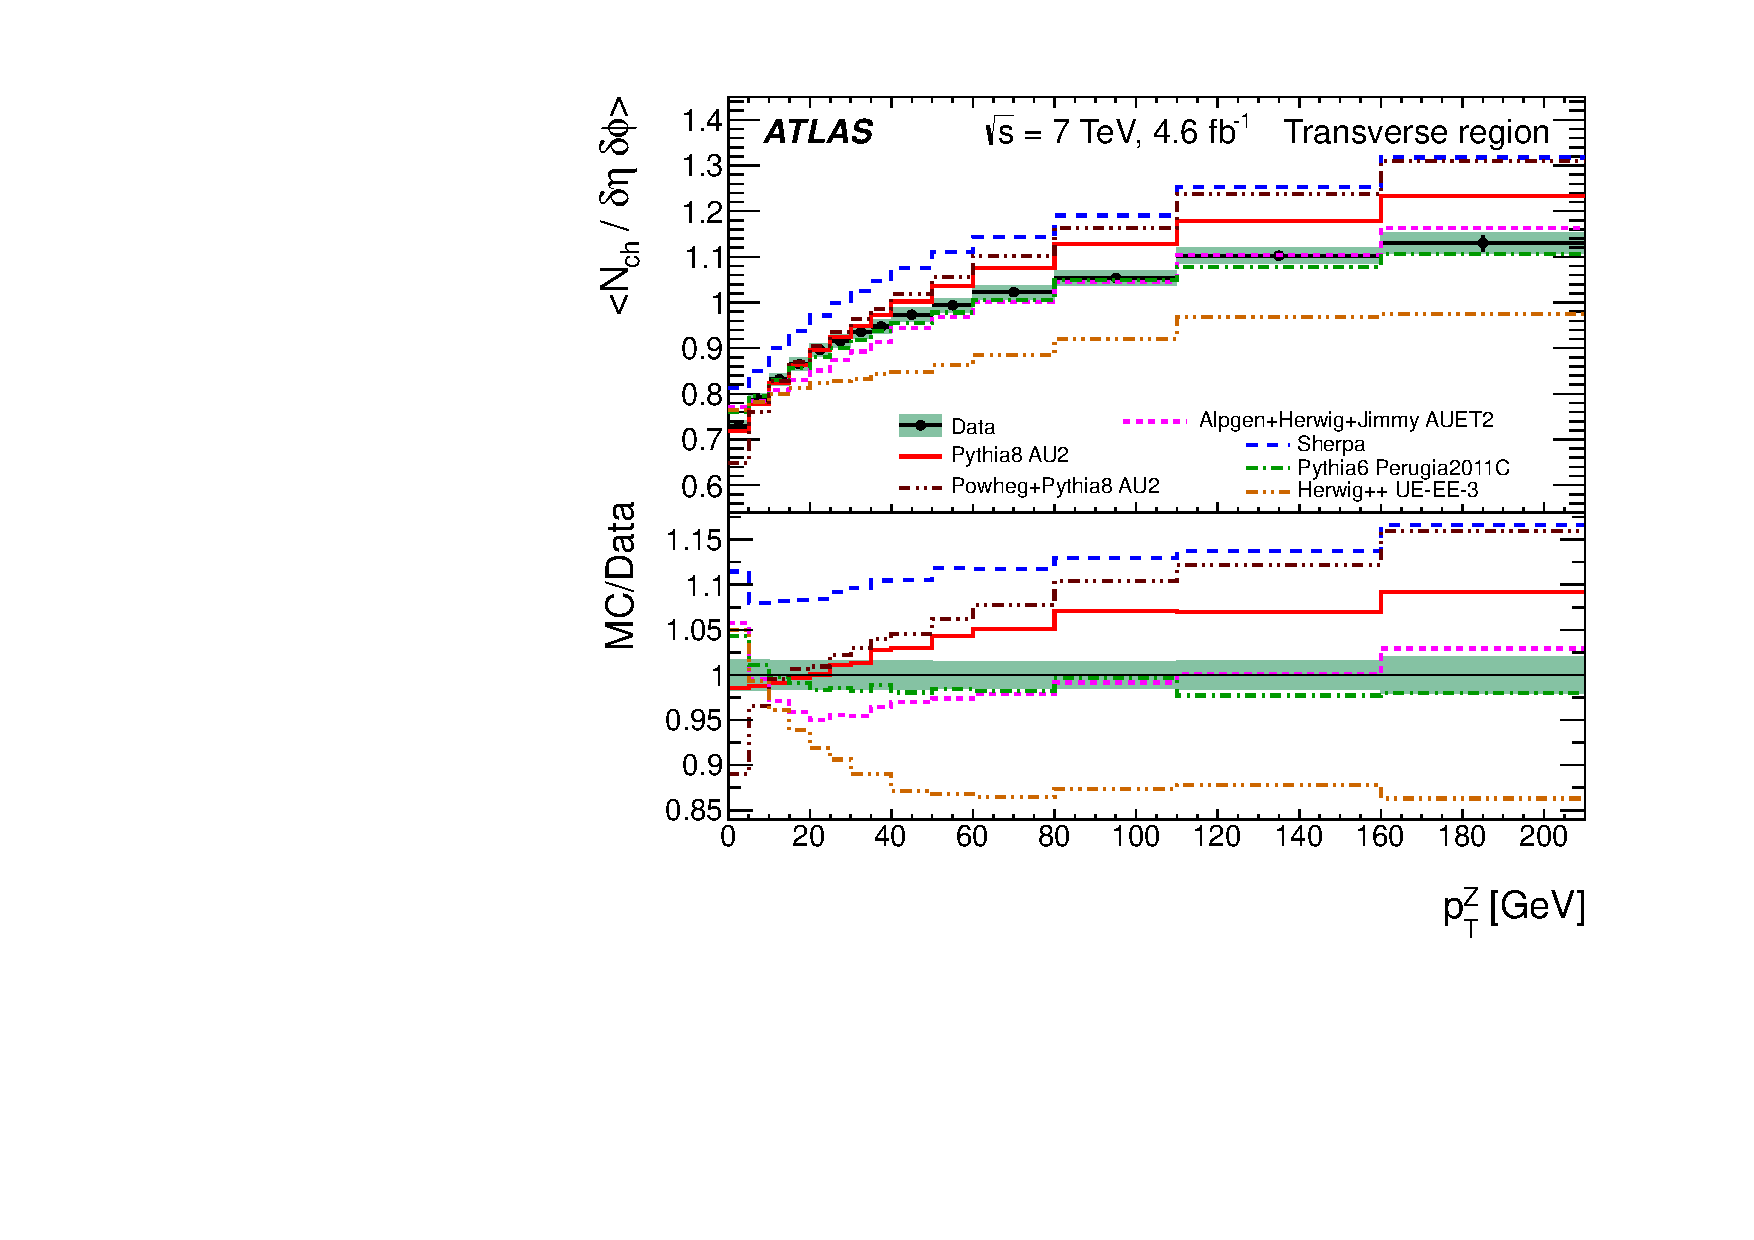
\includegraphics[width=0.48\textwidth]{figures/STDM-2011-42/fig_17b}
  \caption{Variables.}
  \label{fig:backgrounds-zue}
\end{figure}

\begin{figure}[tp]
  \centering
  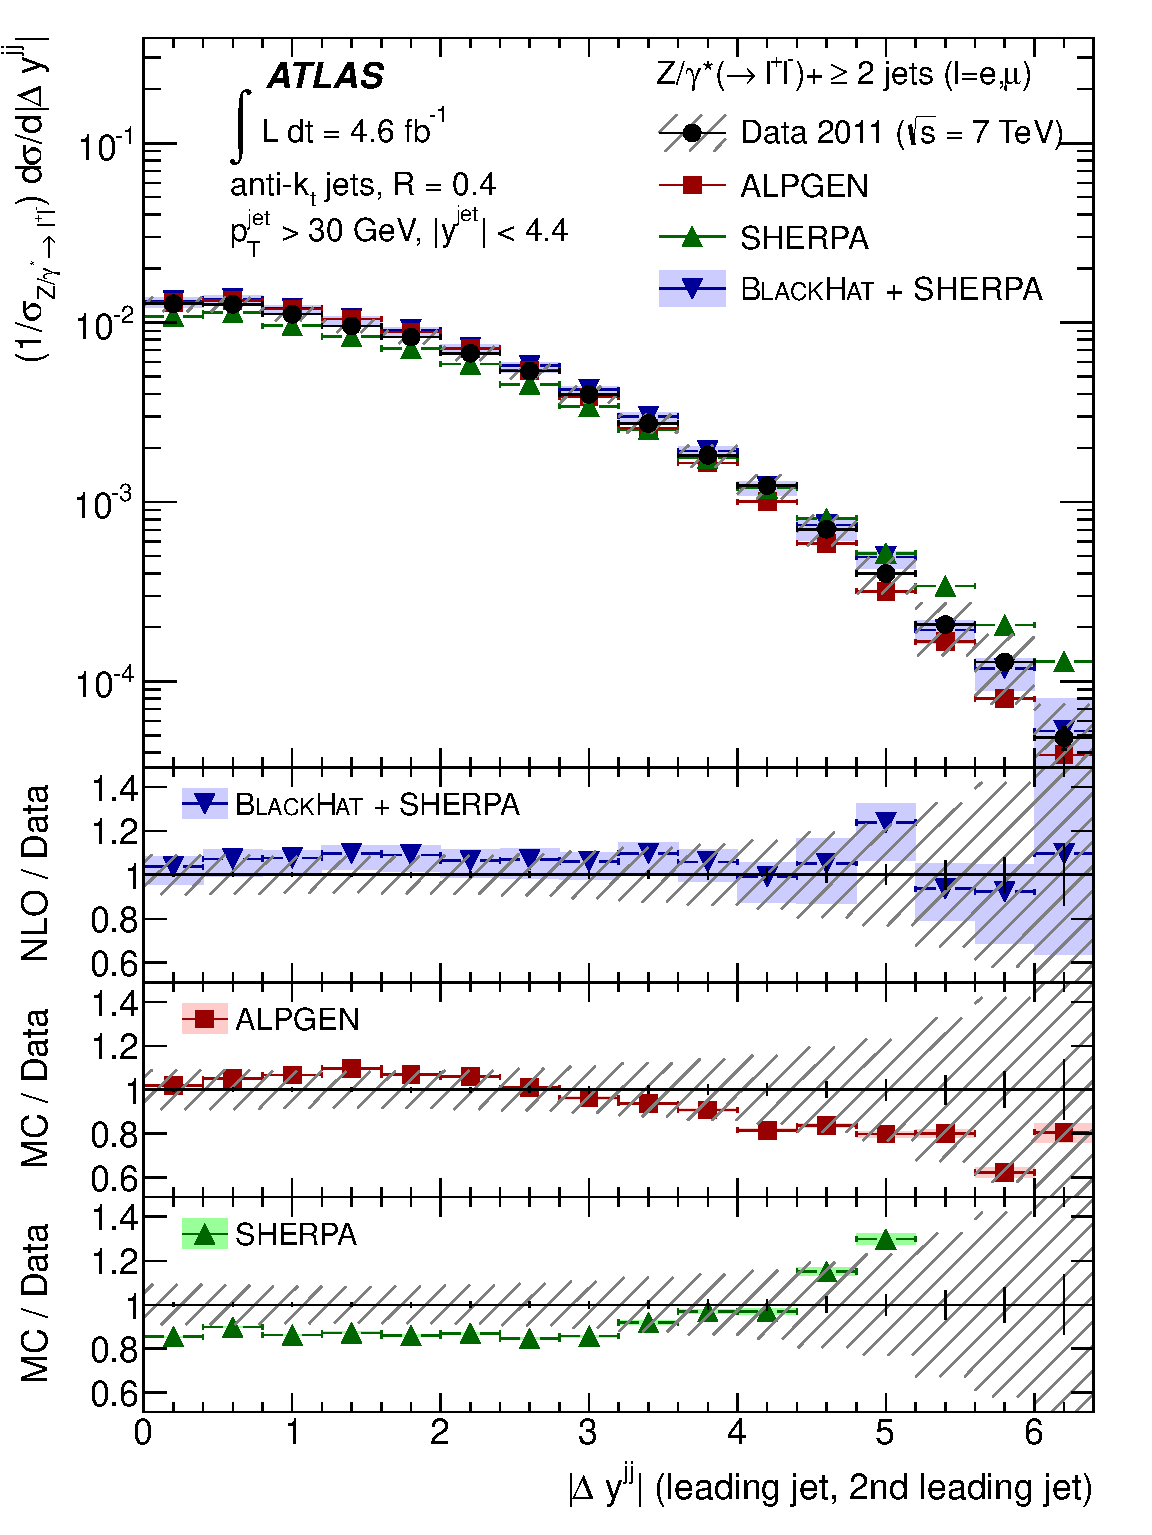
\includegraphics[width=0.32\textwidth]{figures/STDM-2012-04/fig_11a}
  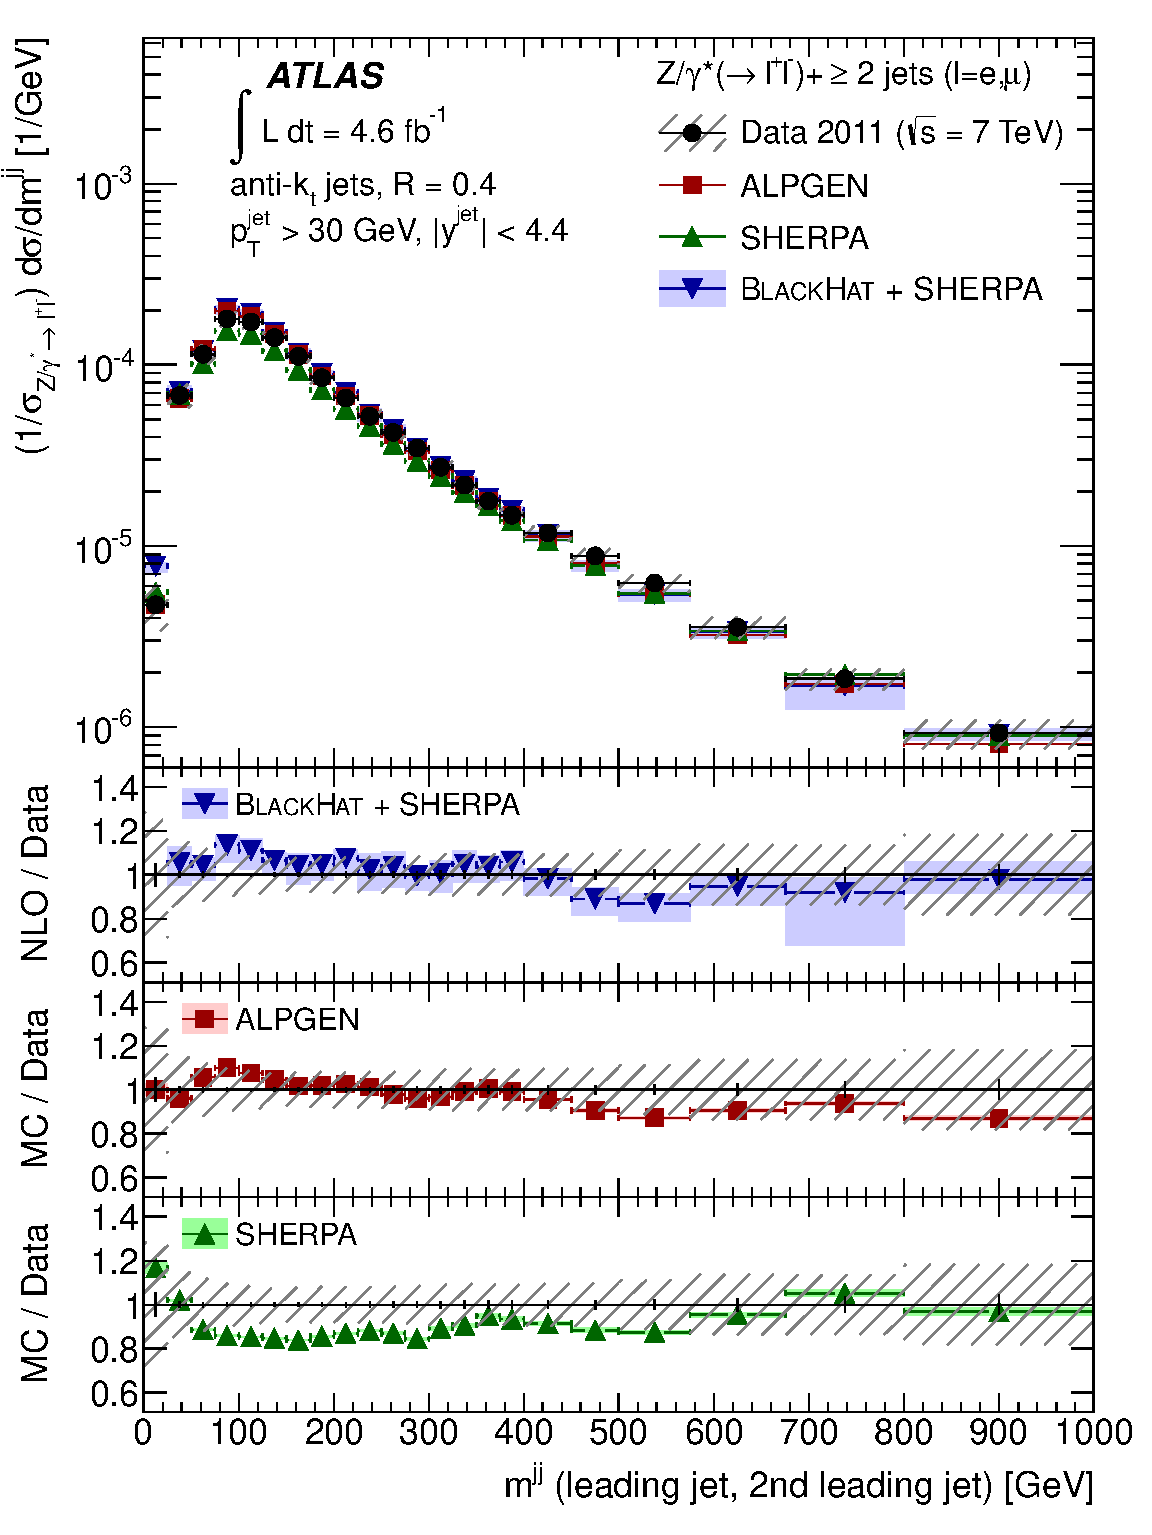
\includegraphics[width=0.32\textwidth]{figures/STDM-2012-04/fig_11b}
  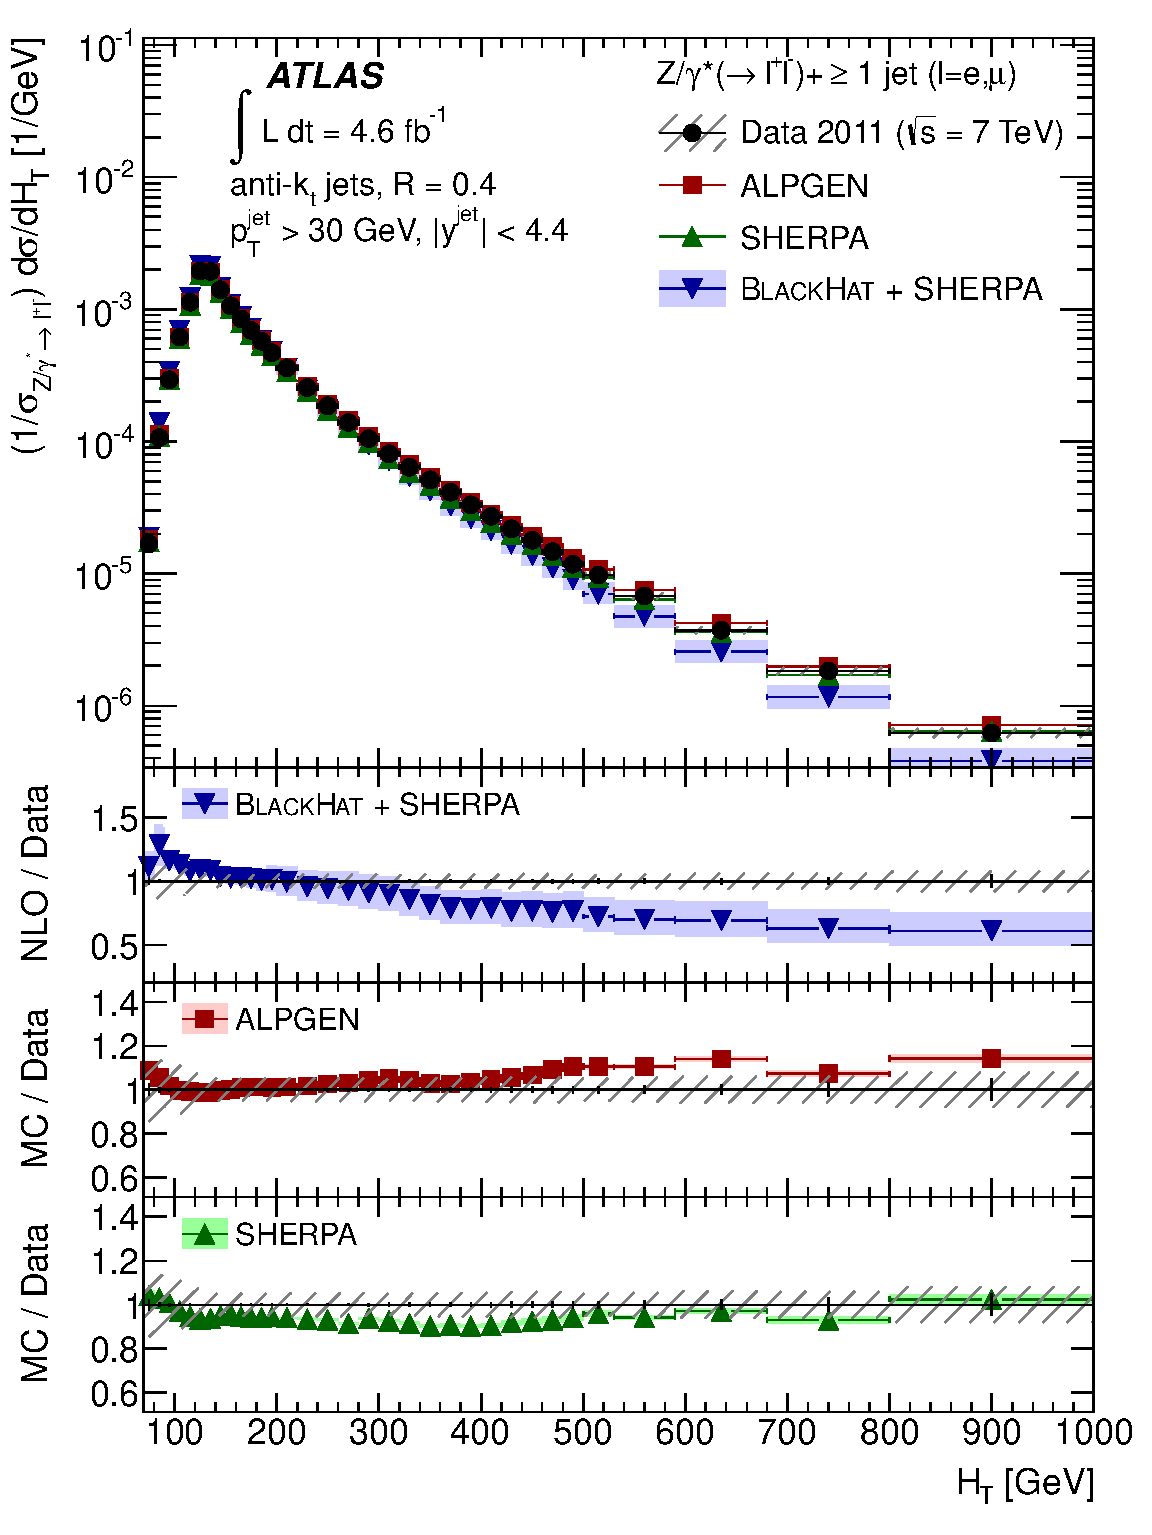
\includegraphics[width=0.32\textwidth]{figures/STDM-2012-04/fig_15a}
  \caption{Variables.}
  \label{fig:backgrounds-zjj}
\end{figure}

\begin{figure}[tp]
  \centering
  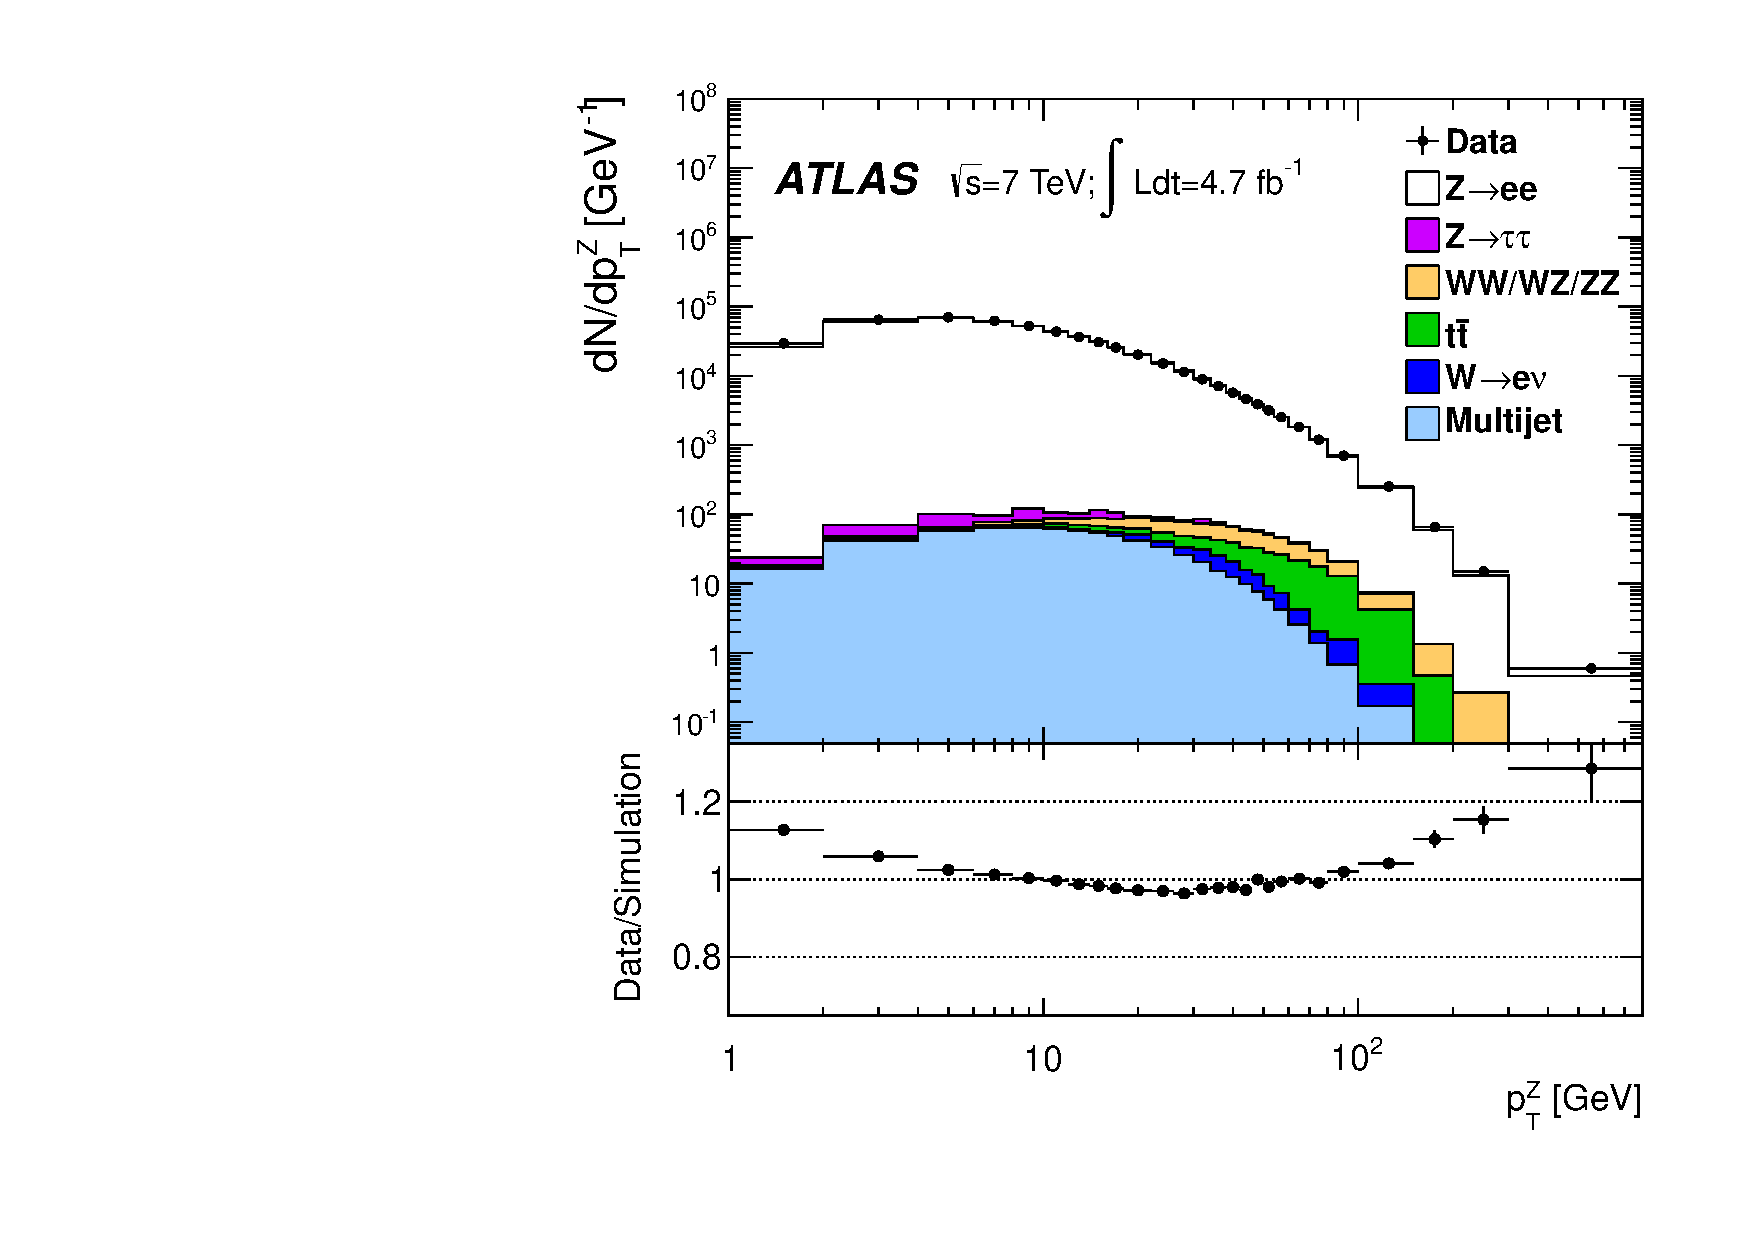
\includegraphics[width=0.48\textwidth]{figures/STDM-2012-23/fig_01a}
  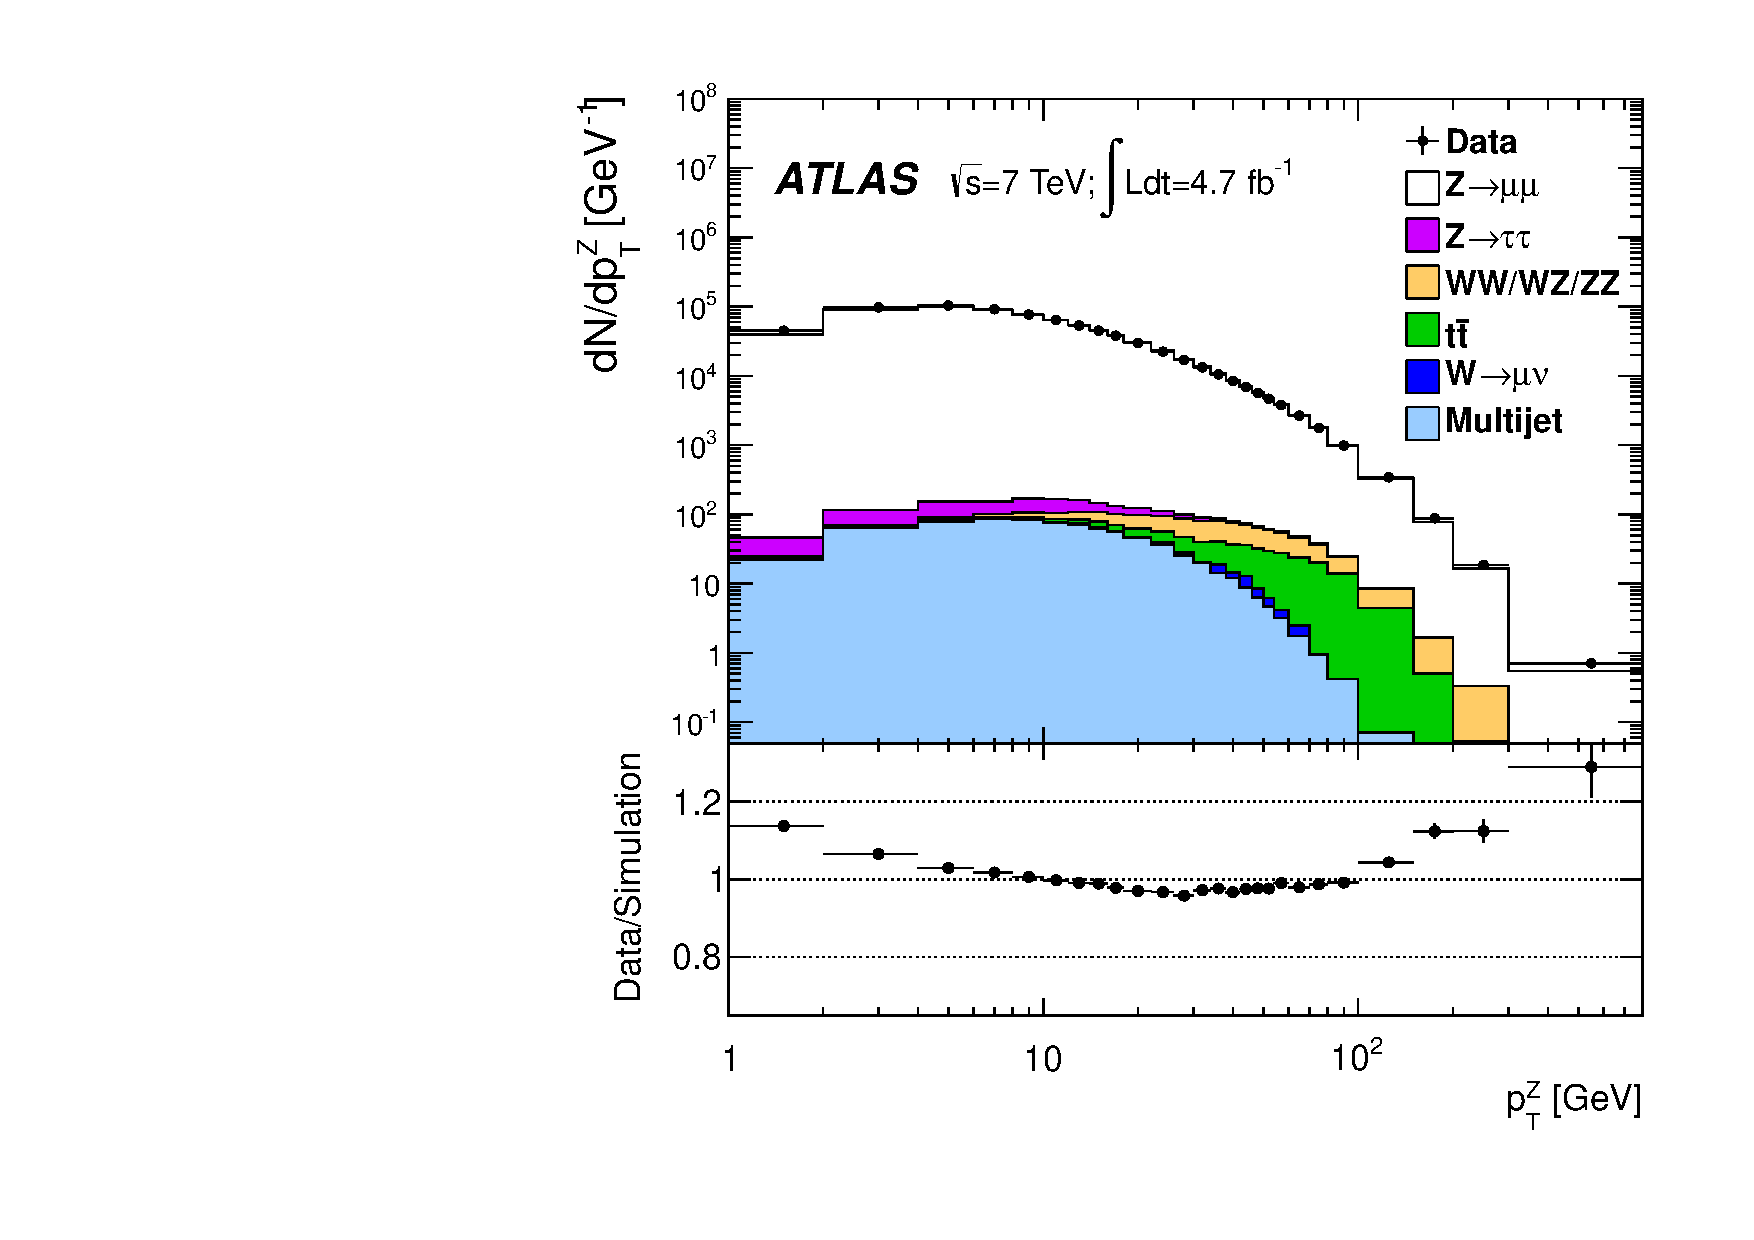
\includegraphics[width=0.48\textwidth]{figures/STDM-2012-23/fig_01b}
  \caption{Variables.}
  \label{fig:backgrounds-zpt}
\end{figure}

\clearpage
\section{$j \rightarrow \tauh$ mis-identification}
\label{sec:backgrounds-misid}

\begin{figure}[tp]
  \centering
  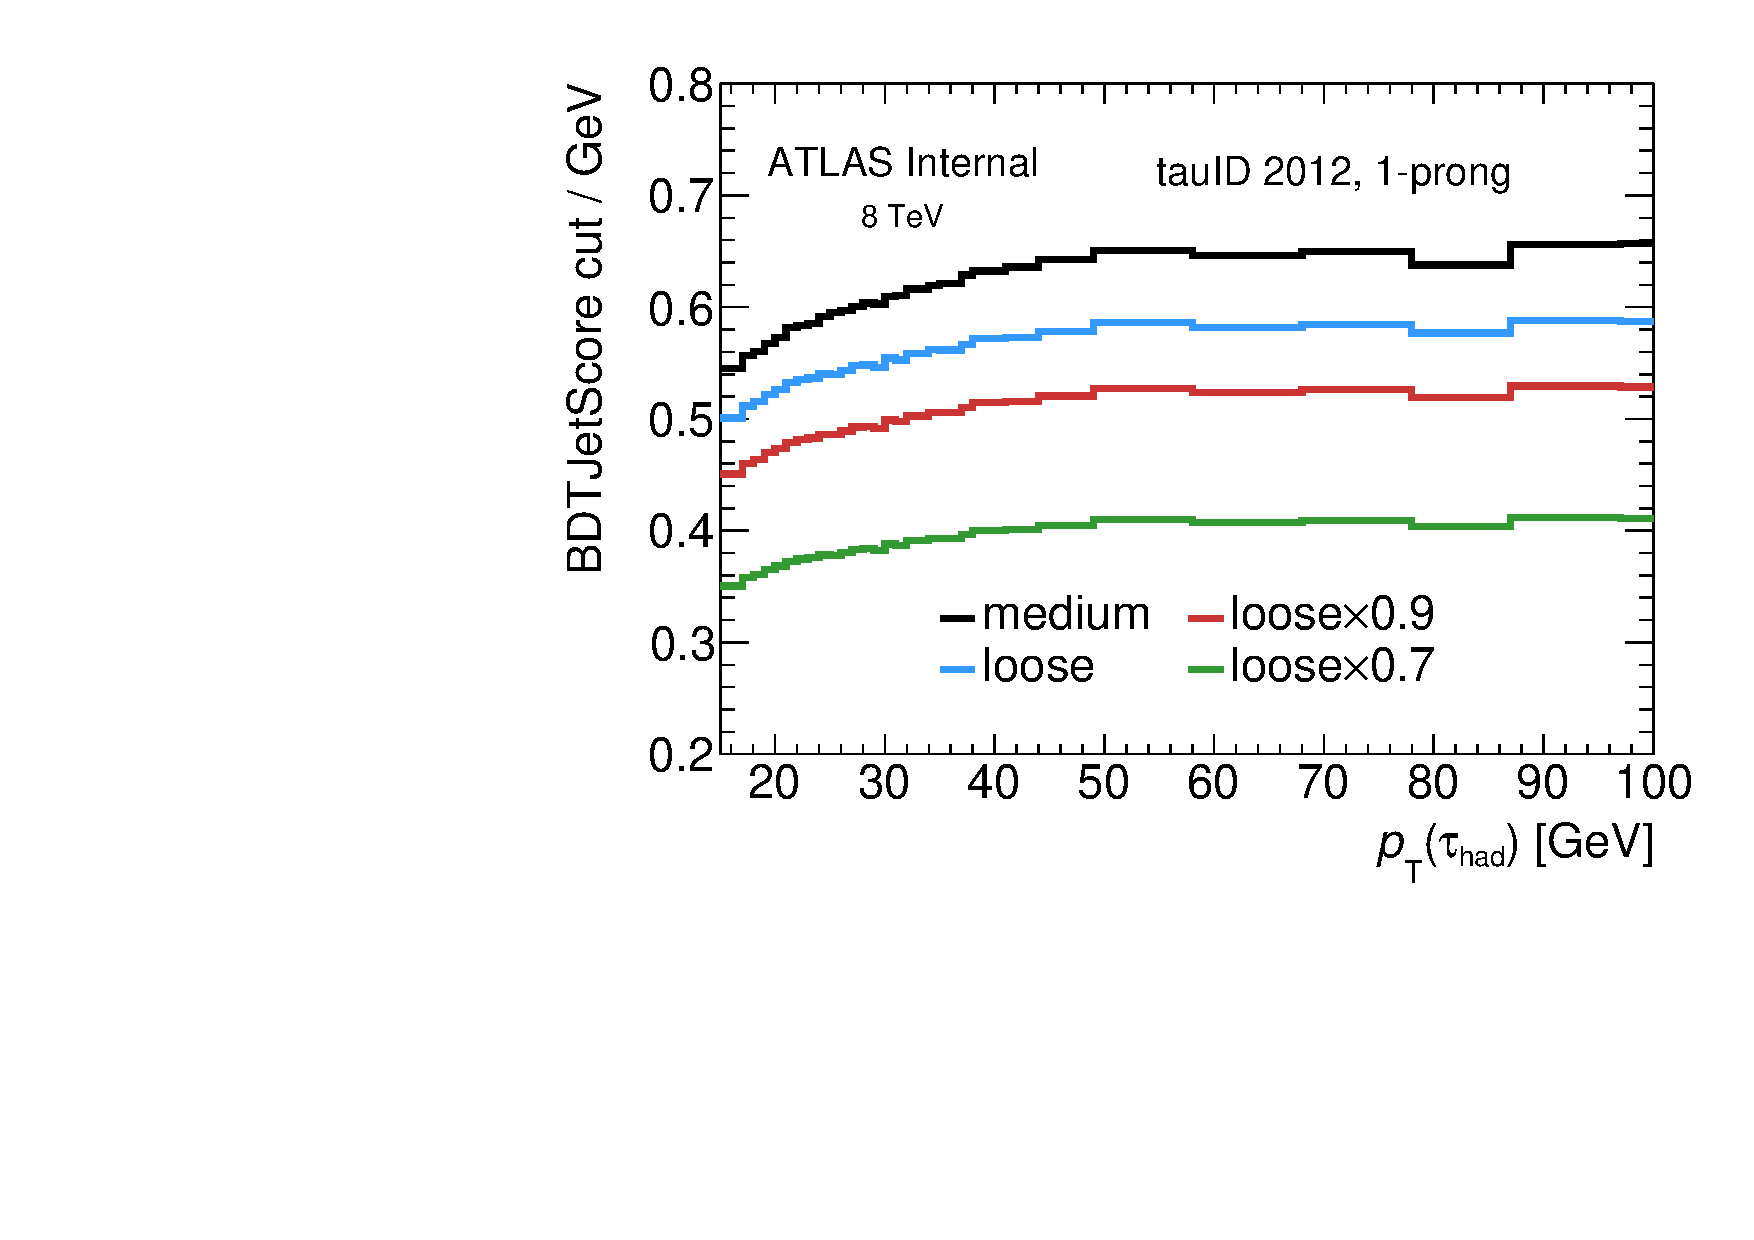
\includegraphics[width=0.48\textwidth]{figures/backgrounds/jetBDT-1p}
  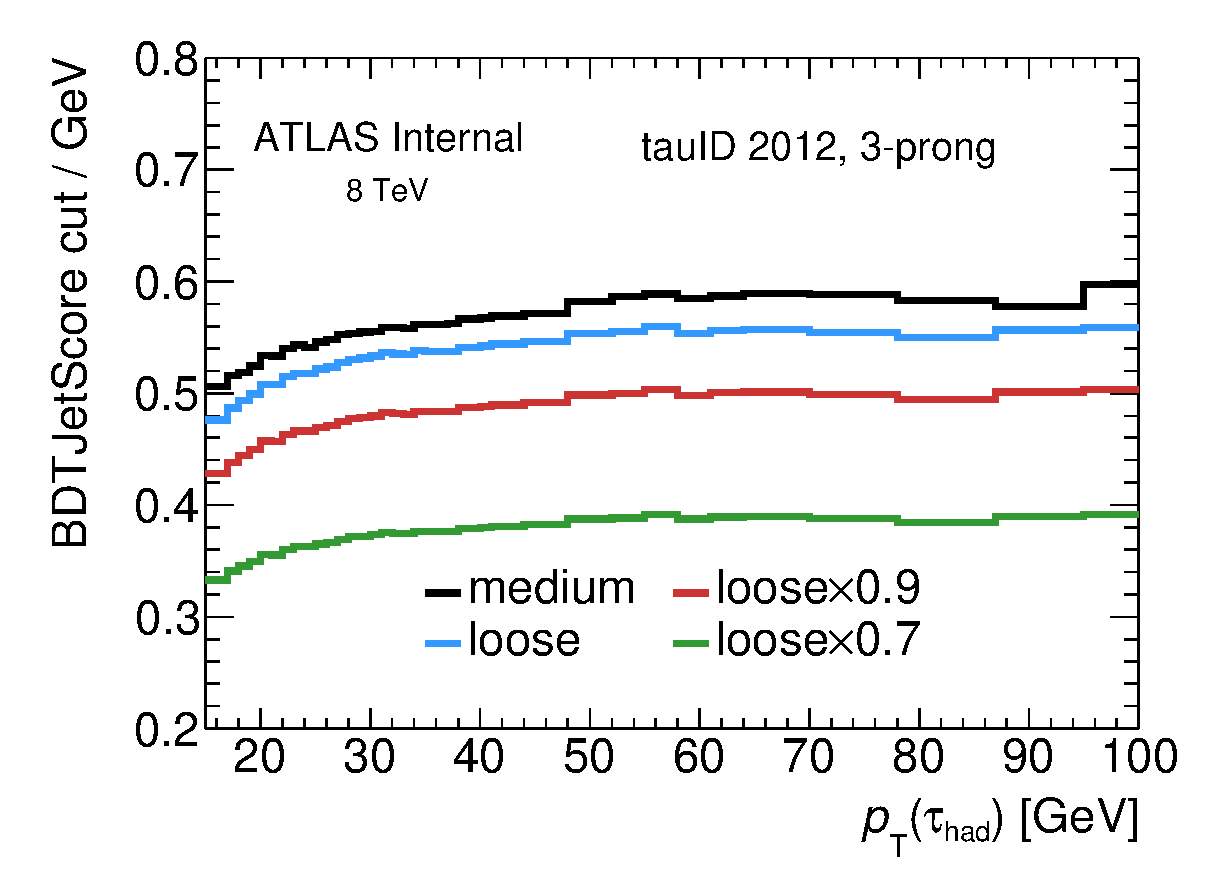
\includegraphics[width=0.48\textwidth]{figures/backgrounds/jetBDT-3p}
  \caption{Variables.}
  \label{fig:backgrounds-workingpoints}
\end{figure}

\begin{figure}[tp]
  \centering
  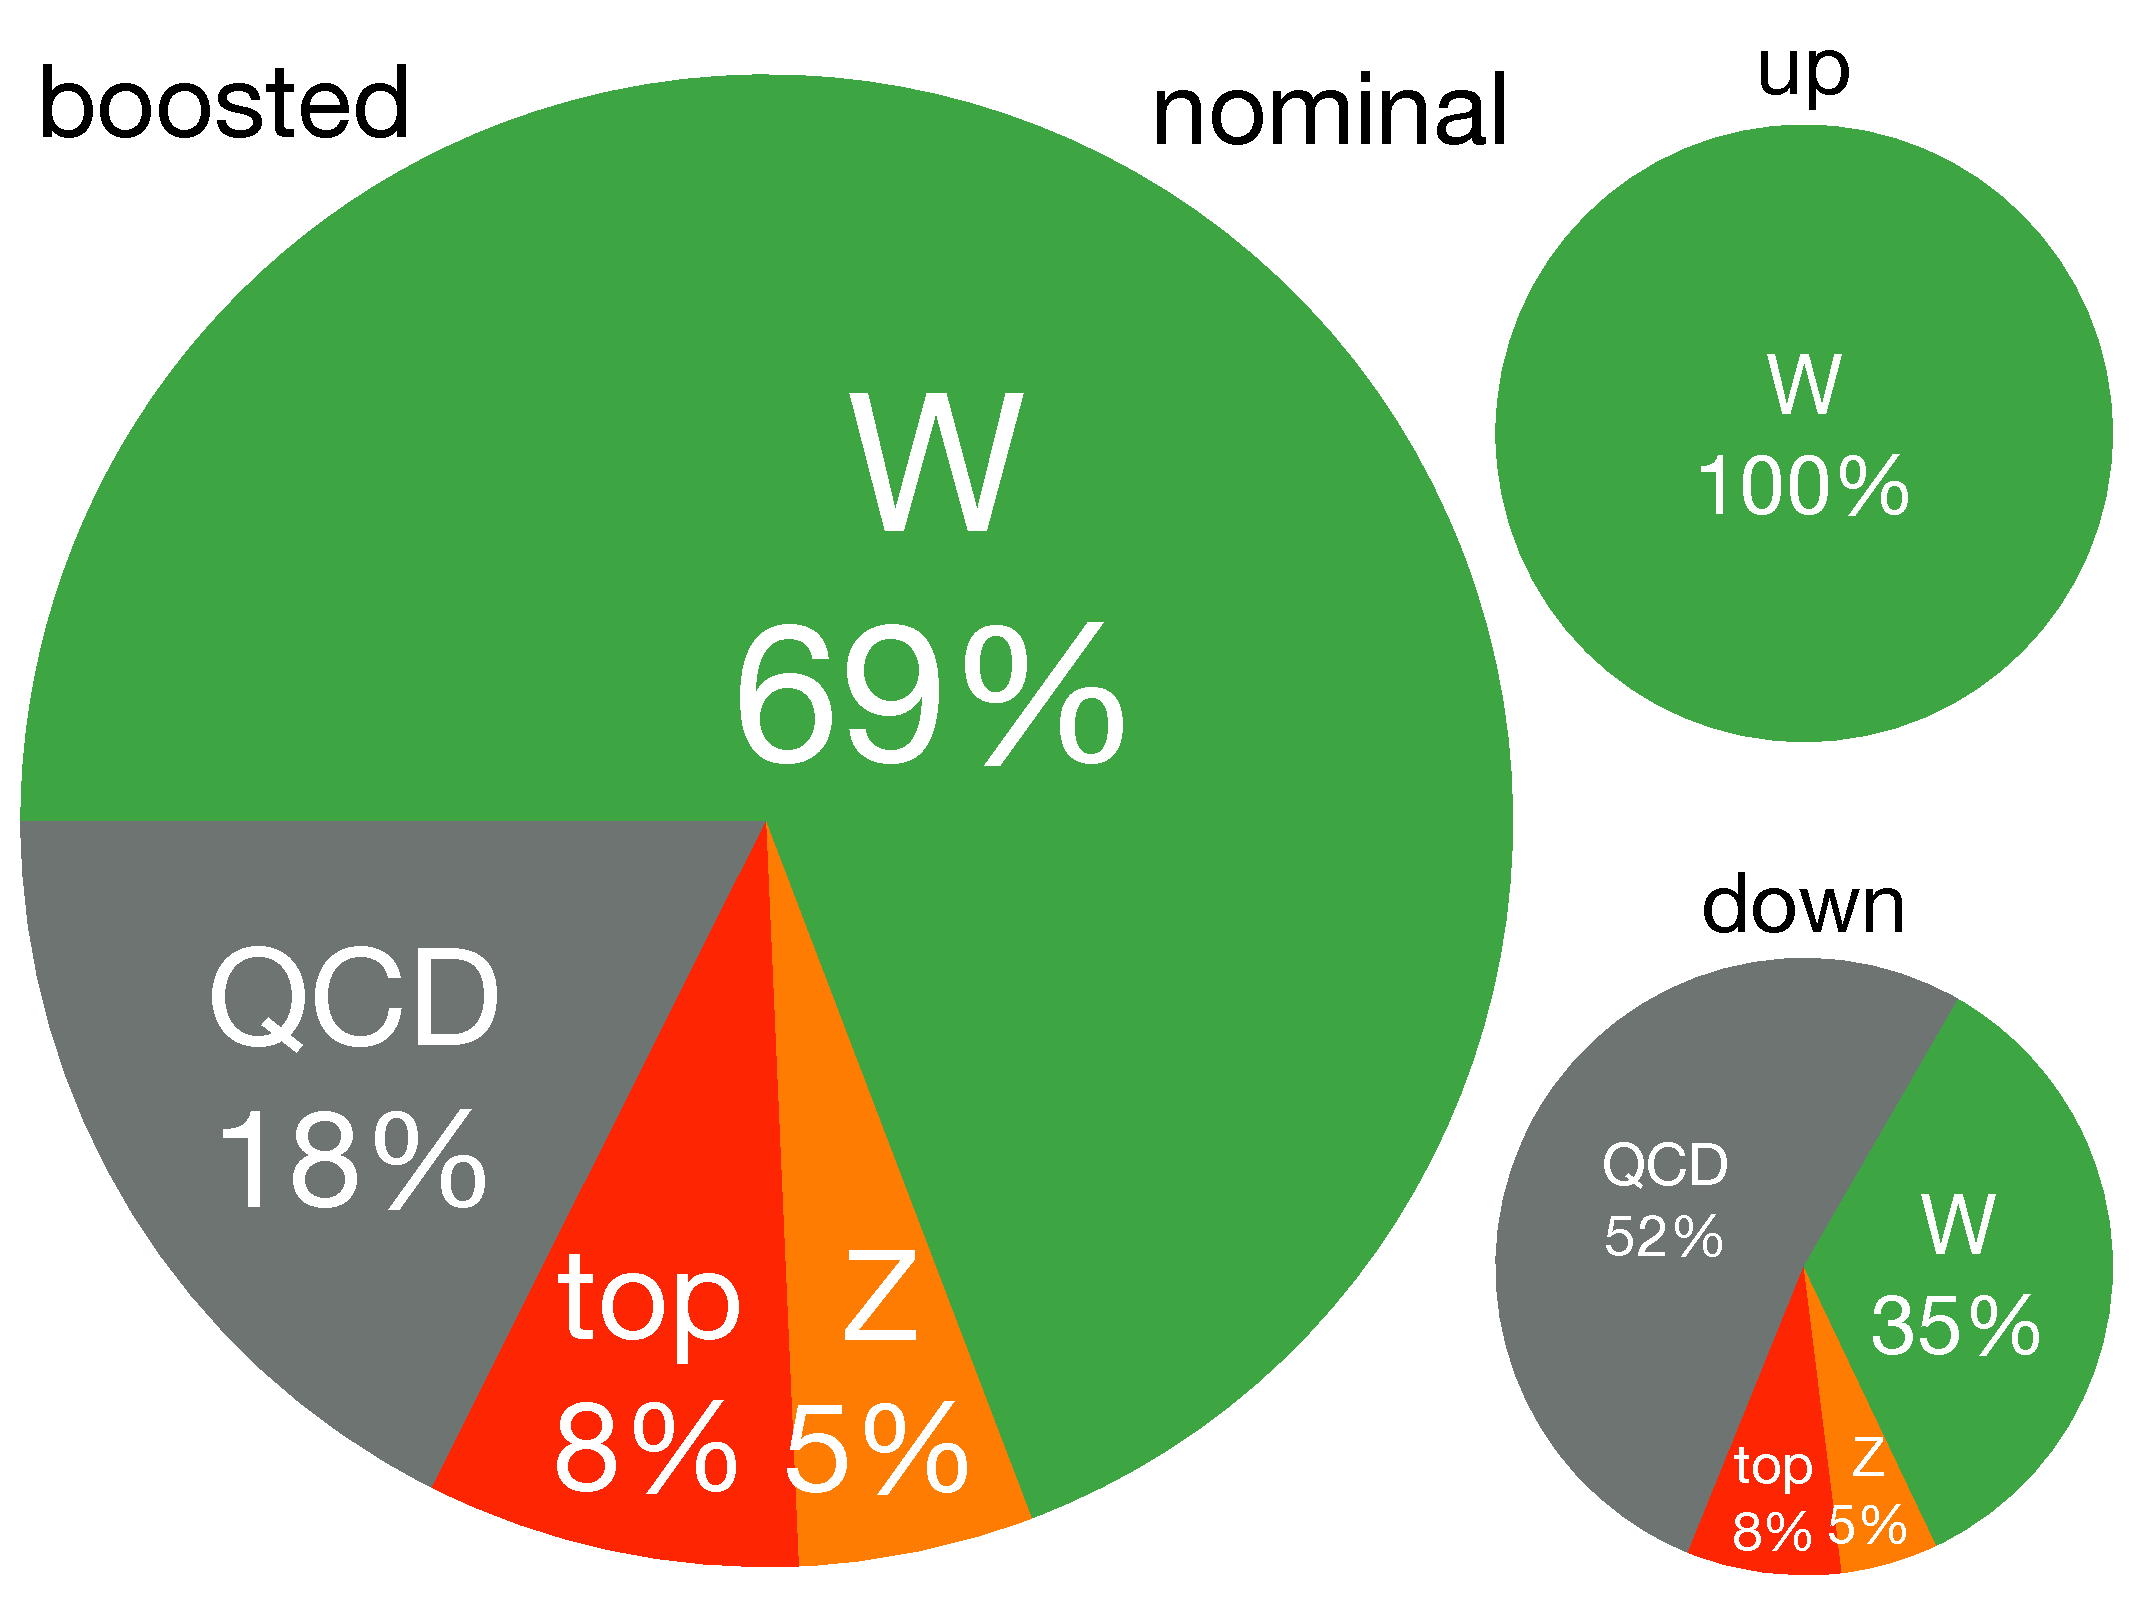
\includegraphics[width=0.90\textwidth]{figures/backgrounds/rx-boost}
  \caption{Variables.}
  \label{fig:backgrounds-rx-boost}
\end{figure}

\begin{figure}[tp]
  \centering
  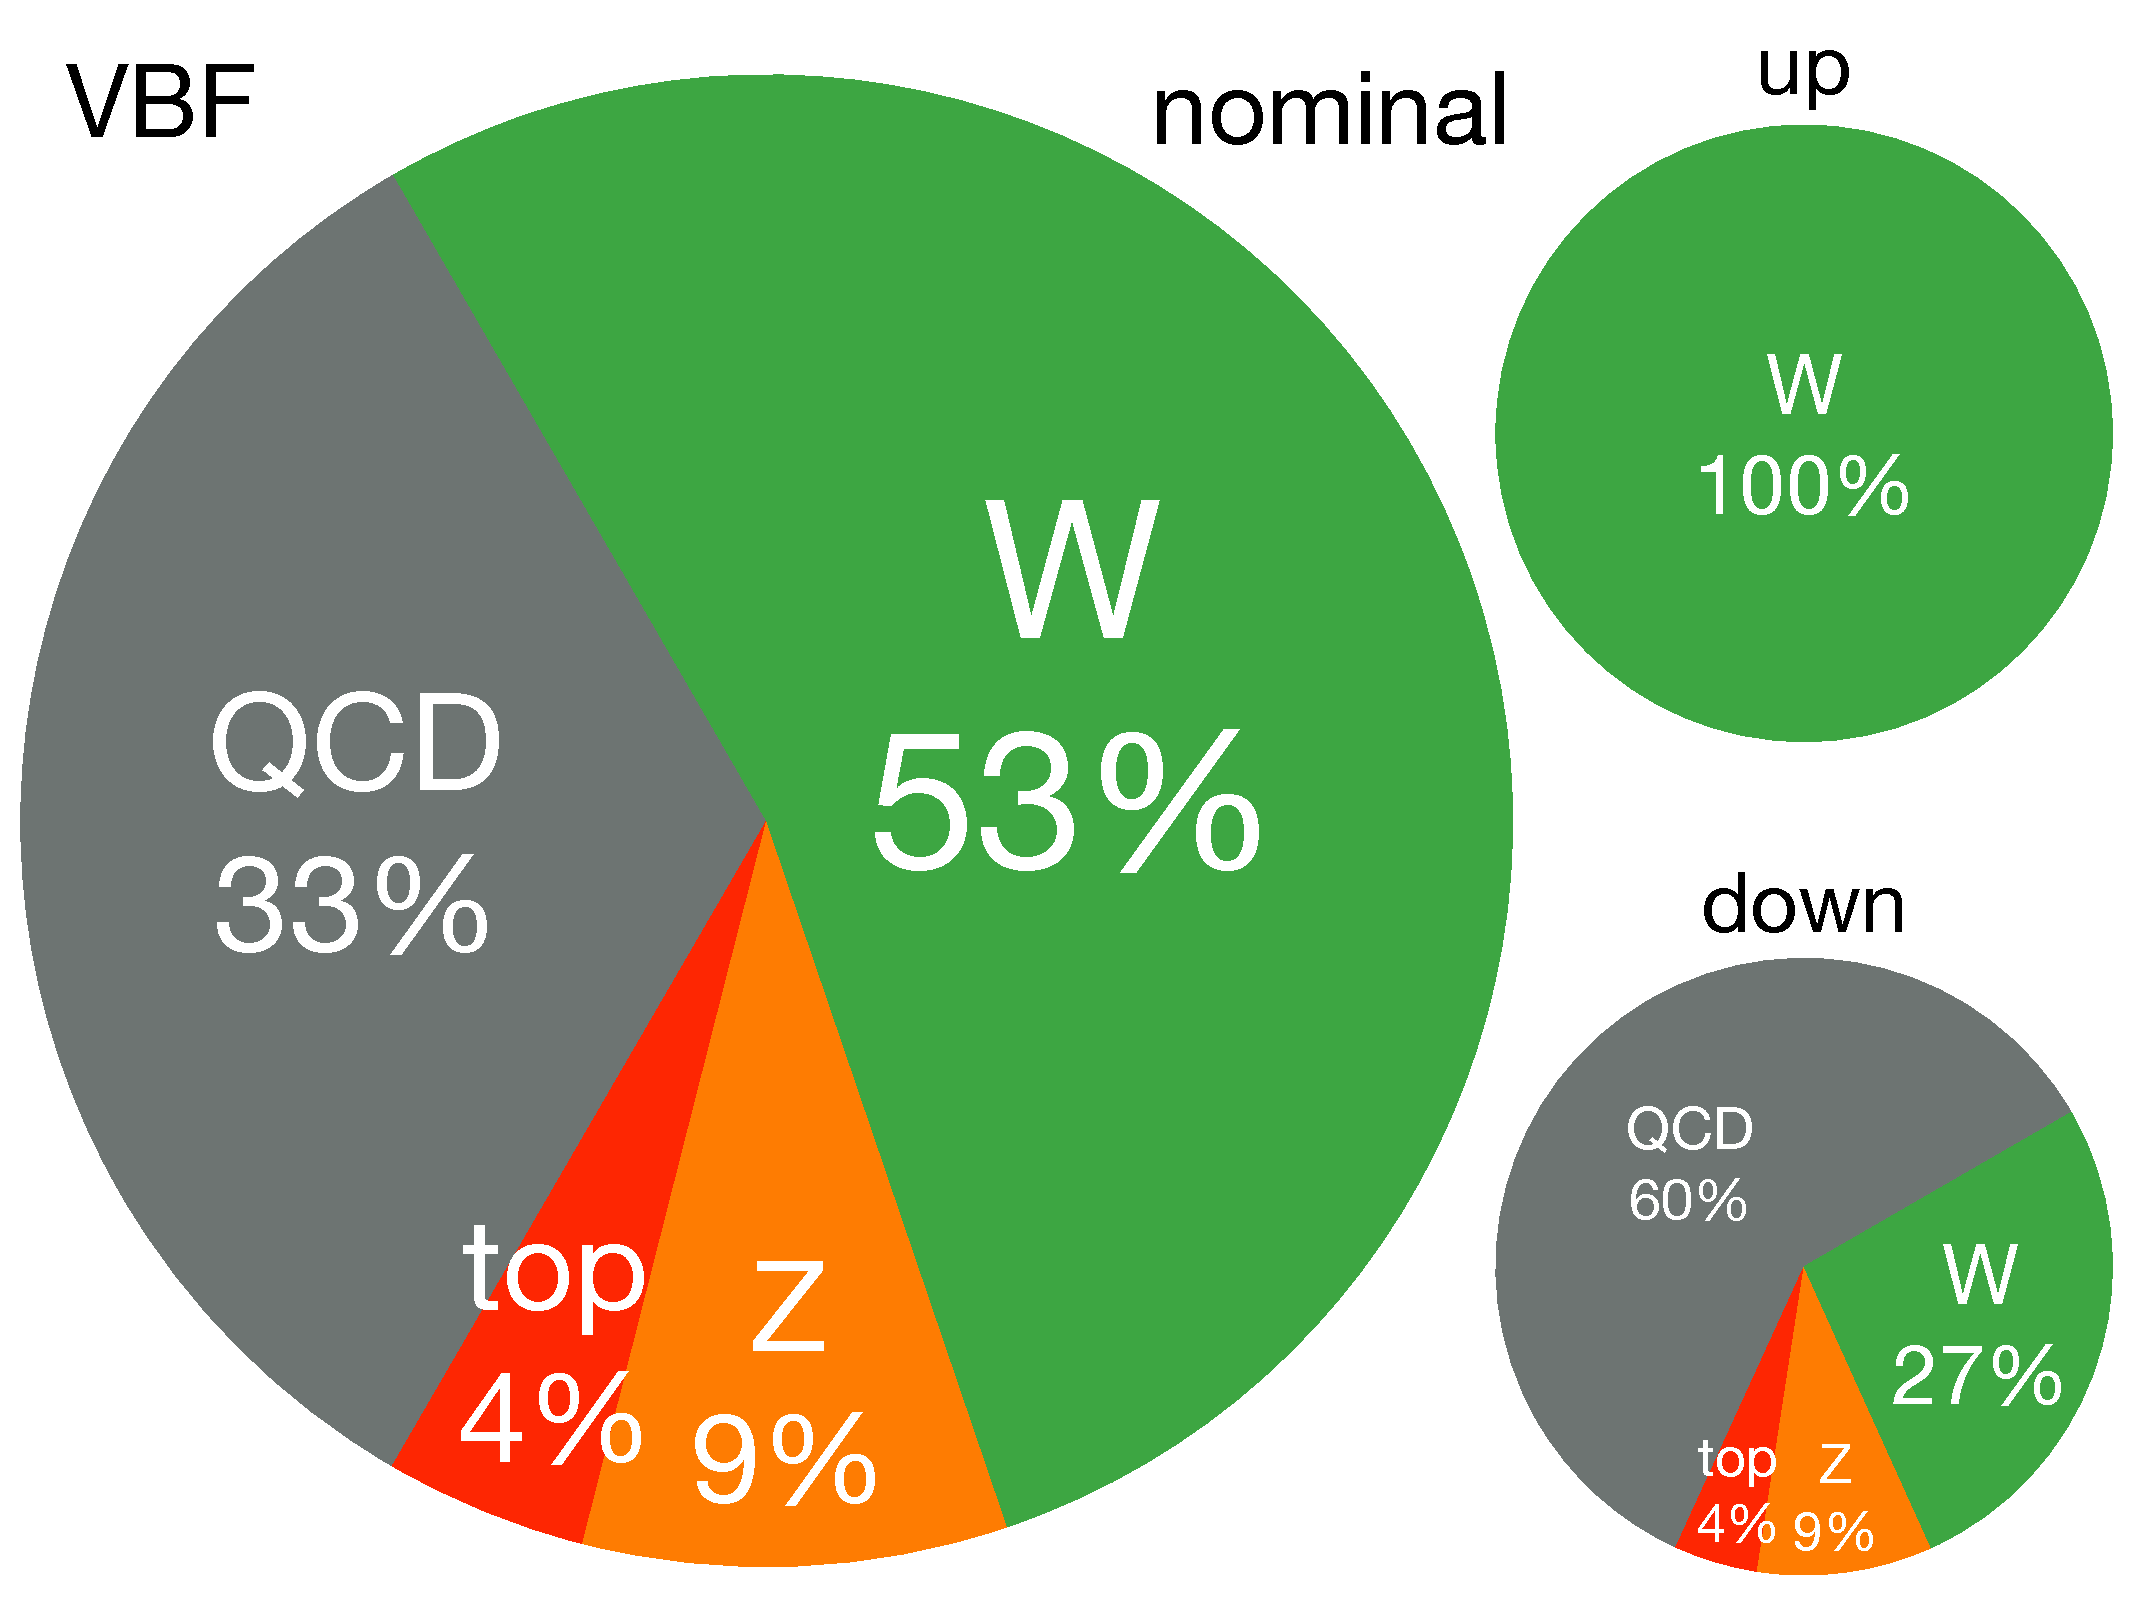
\includegraphics[width=0.90\textwidth]{figures/backgrounds/rx-vbf}
  \caption{Variables.}
  \label{fig:backgrounds-rx-vbf}
\end{figure}

\begin{figure}[tp]
  \centering
  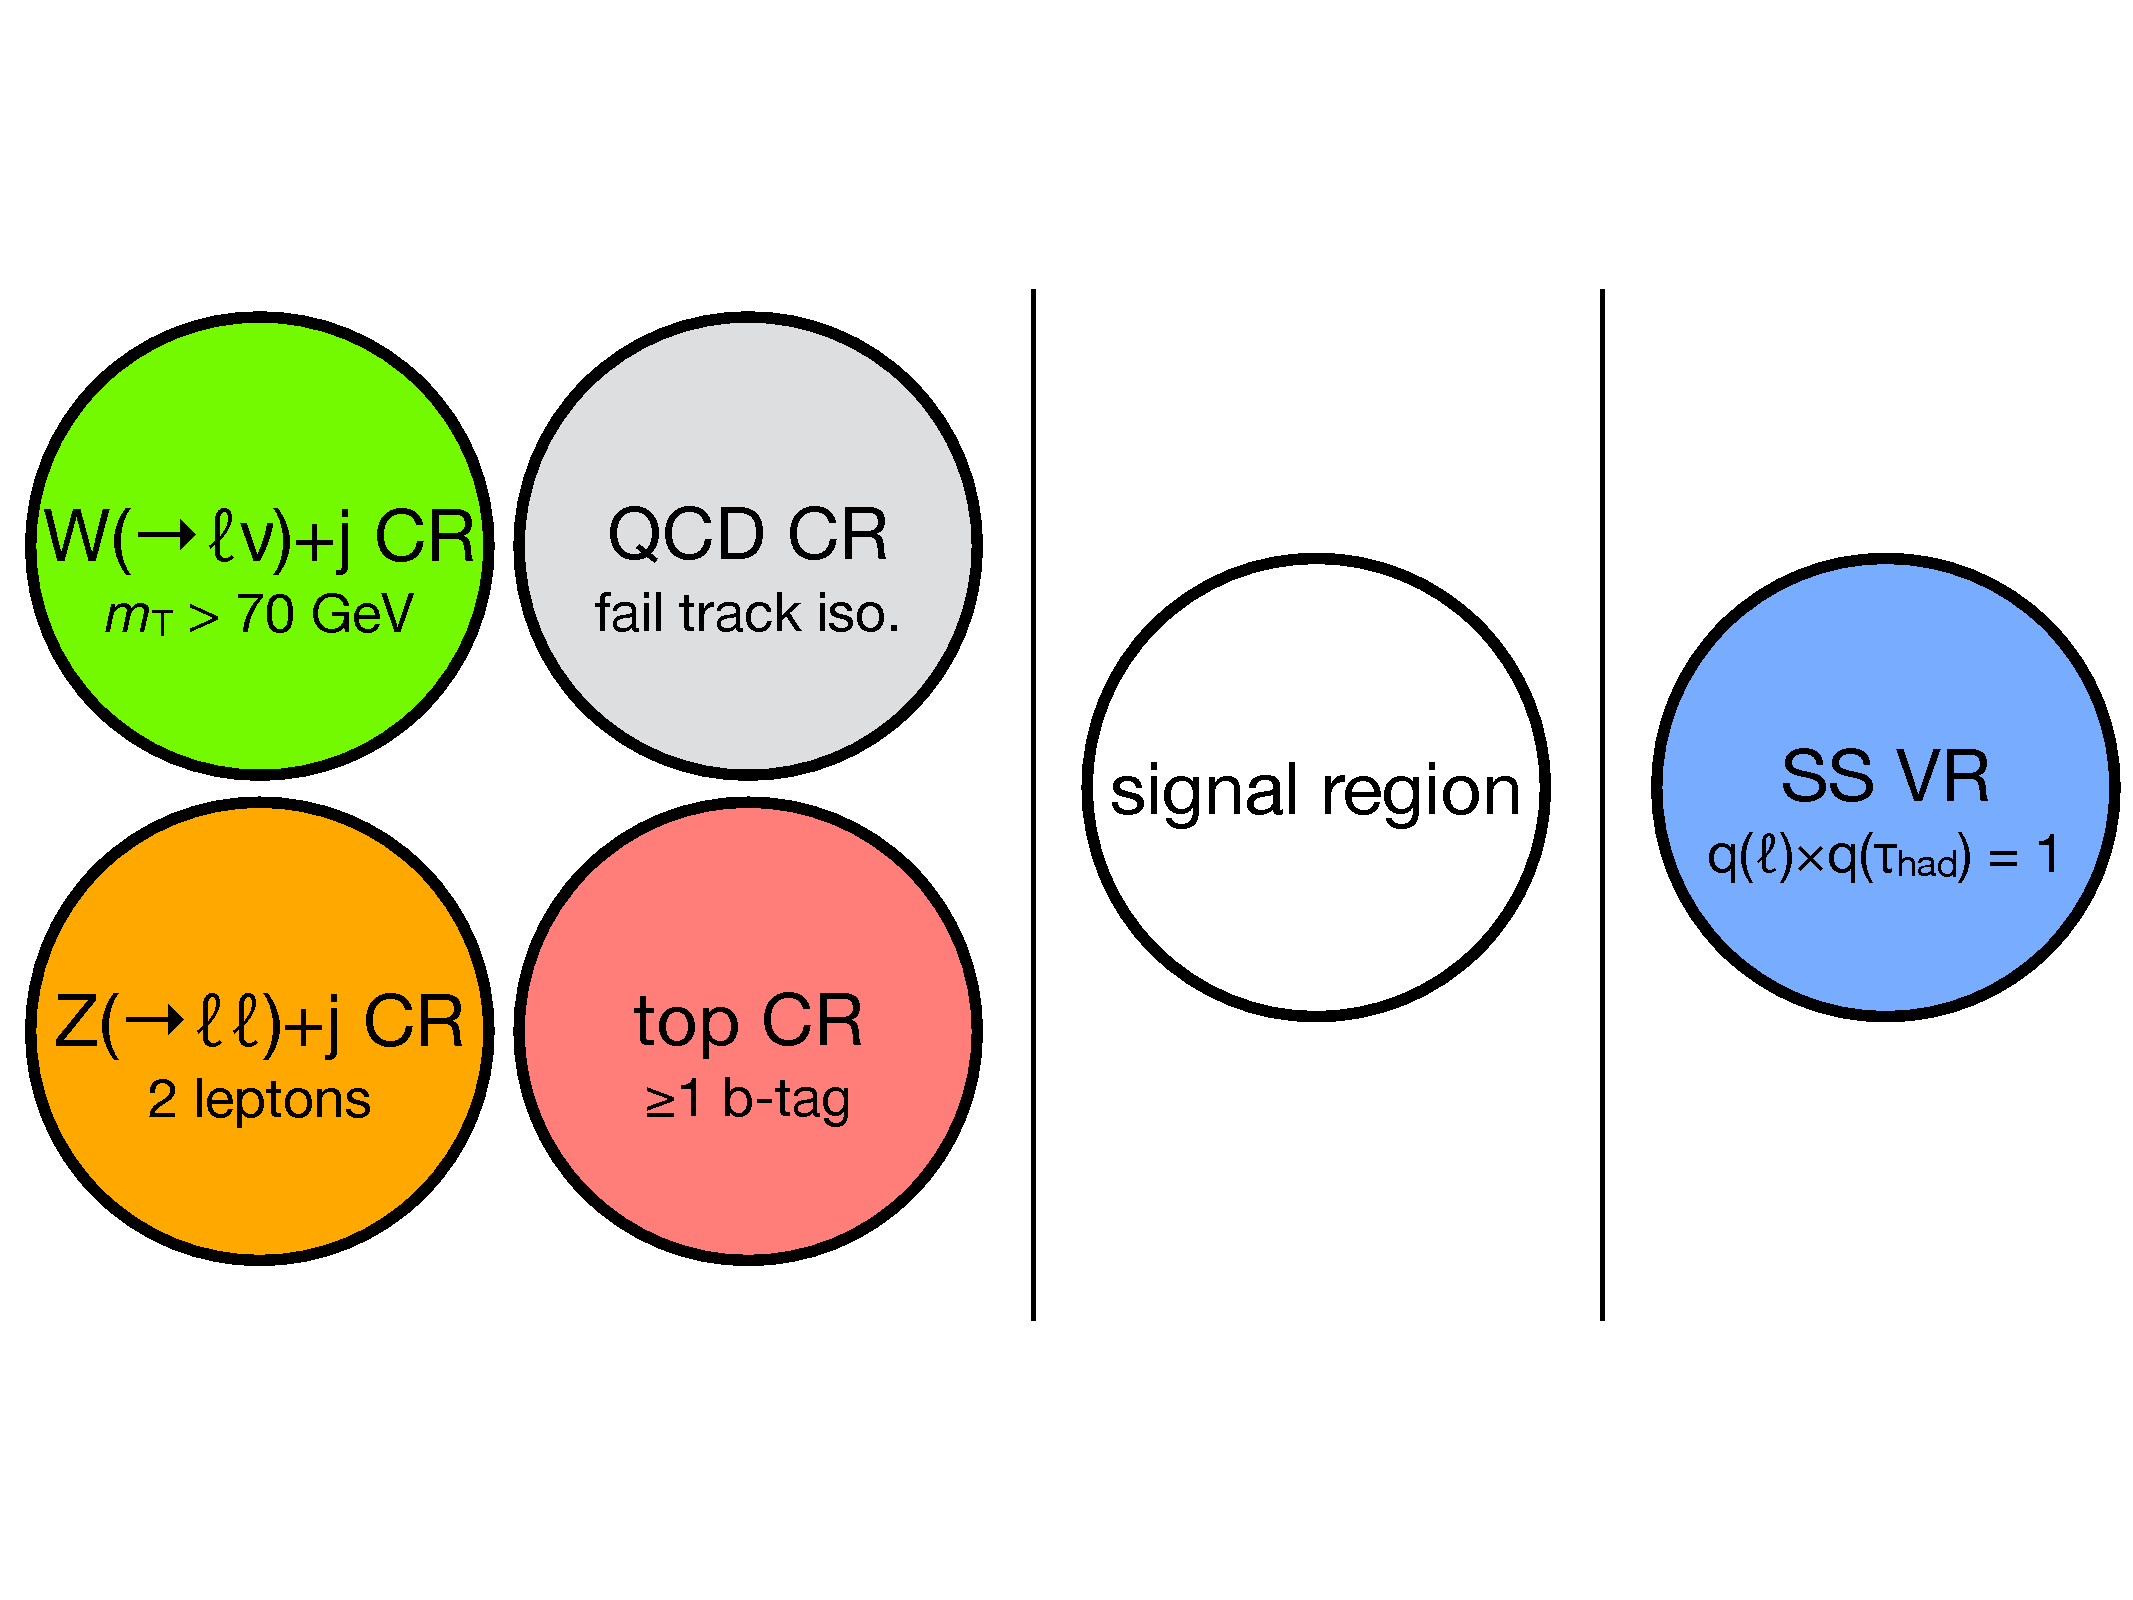
\includegraphics[width=0.90\textwidth]{figures/backgrounds/regions-cartoon}
  \caption{Variables.}
  \label{fig:backgrounds-regions}
\end{figure}

\begin{figure}[tp]
  \centering
  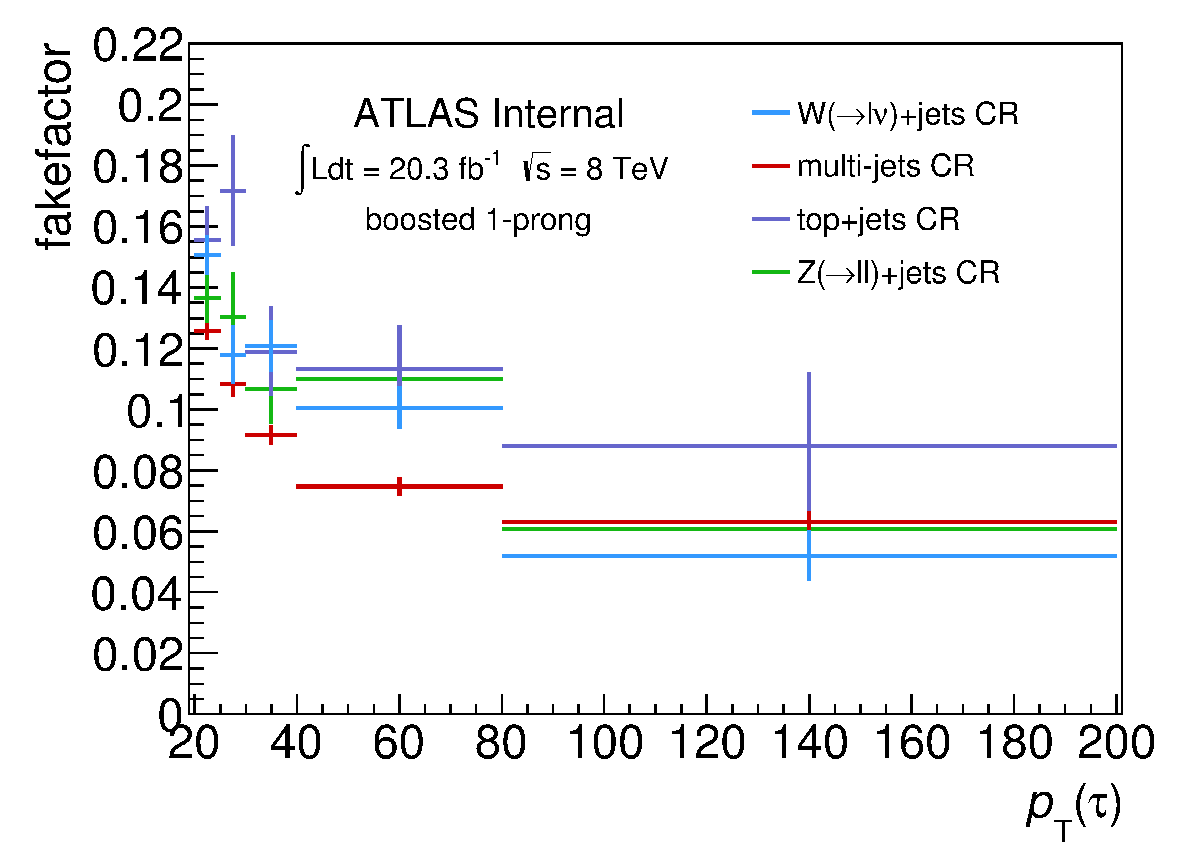
\includegraphics[width=0.48\textwidth]{figures/backgrounds/fakefactor_8TeV_boosted_1p_CRs}
  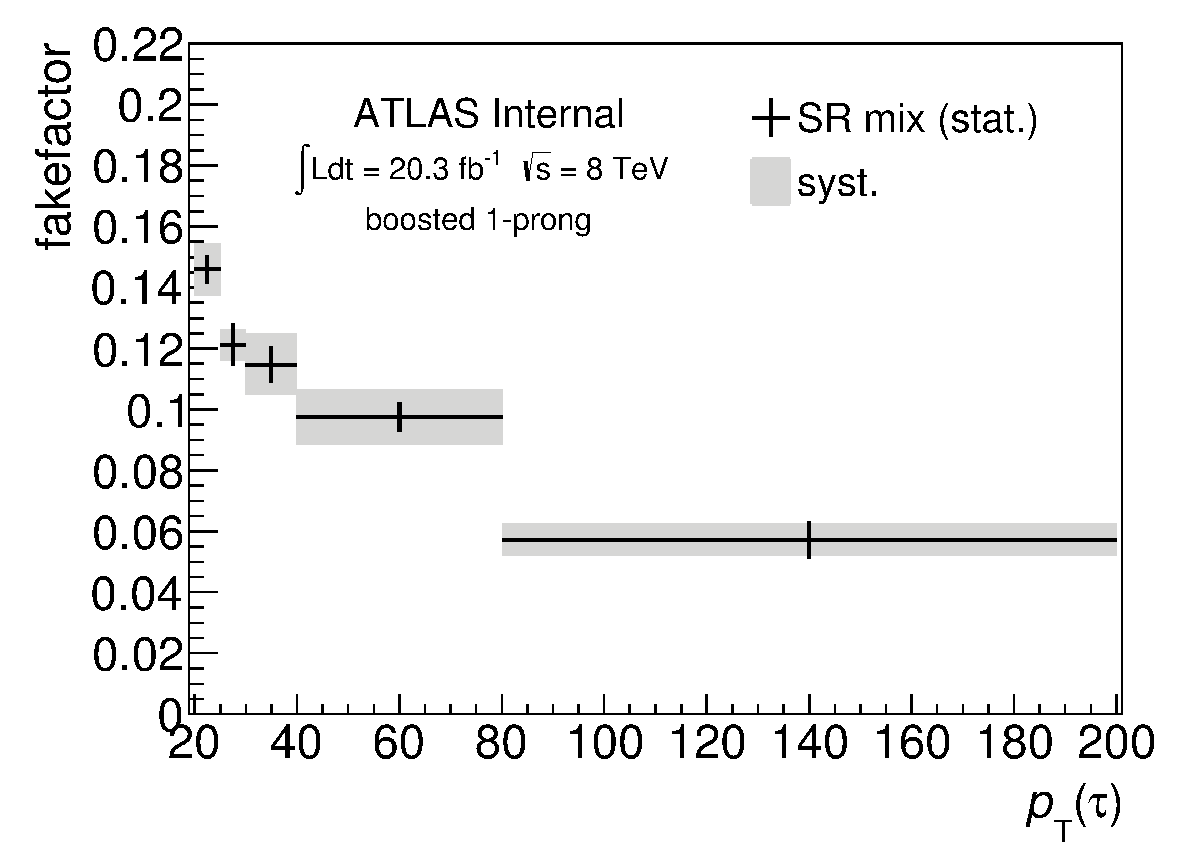
\includegraphics[width=0.48\textwidth]{figures/backgrounds/fakefactor_8TeV_boosted_1p_mix}
  \caption{Variables.}
  \label{fig:backgrounds-fakefactorsboost1p}
\end{figure}

\begin{figure}[tp]
  \centering
  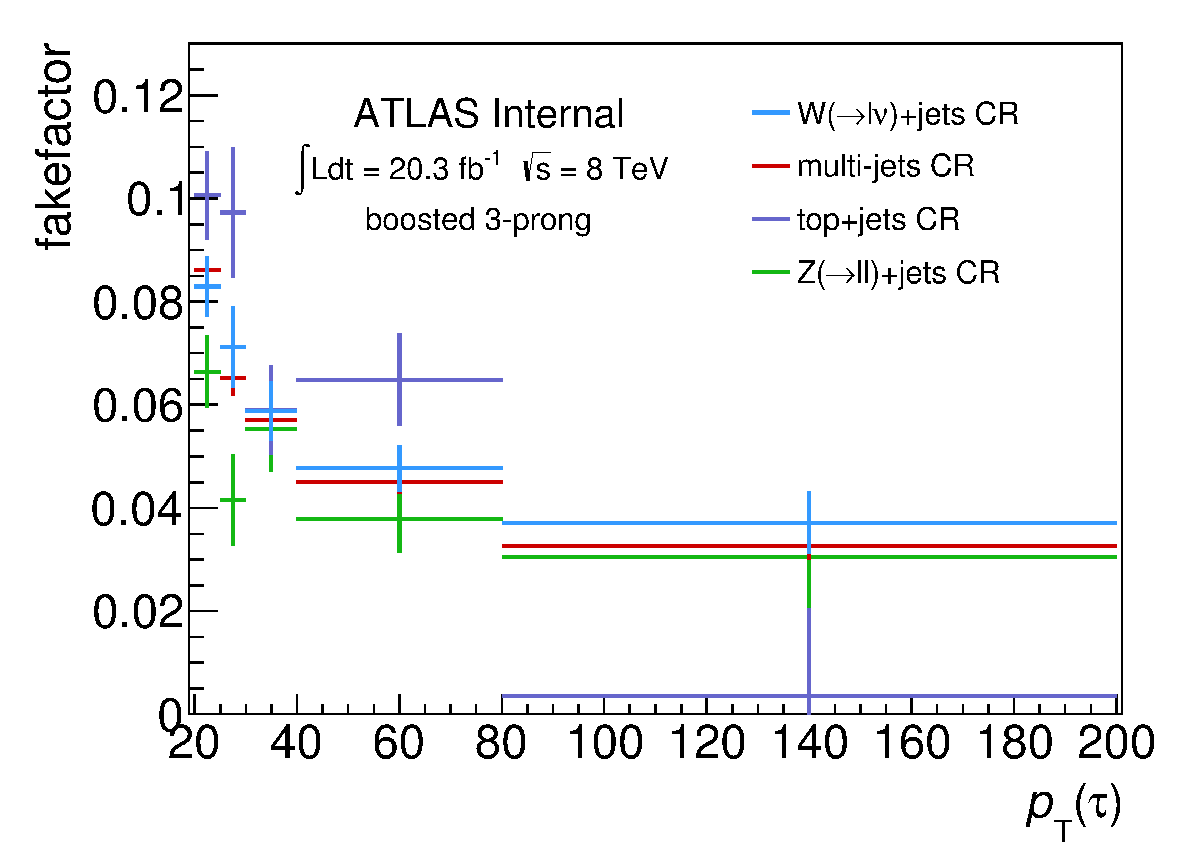
\includegraphics[width=0.48\textwidth]{figures/backgrounds/fakefactor_8TeV_boosted_3p_CRs}
  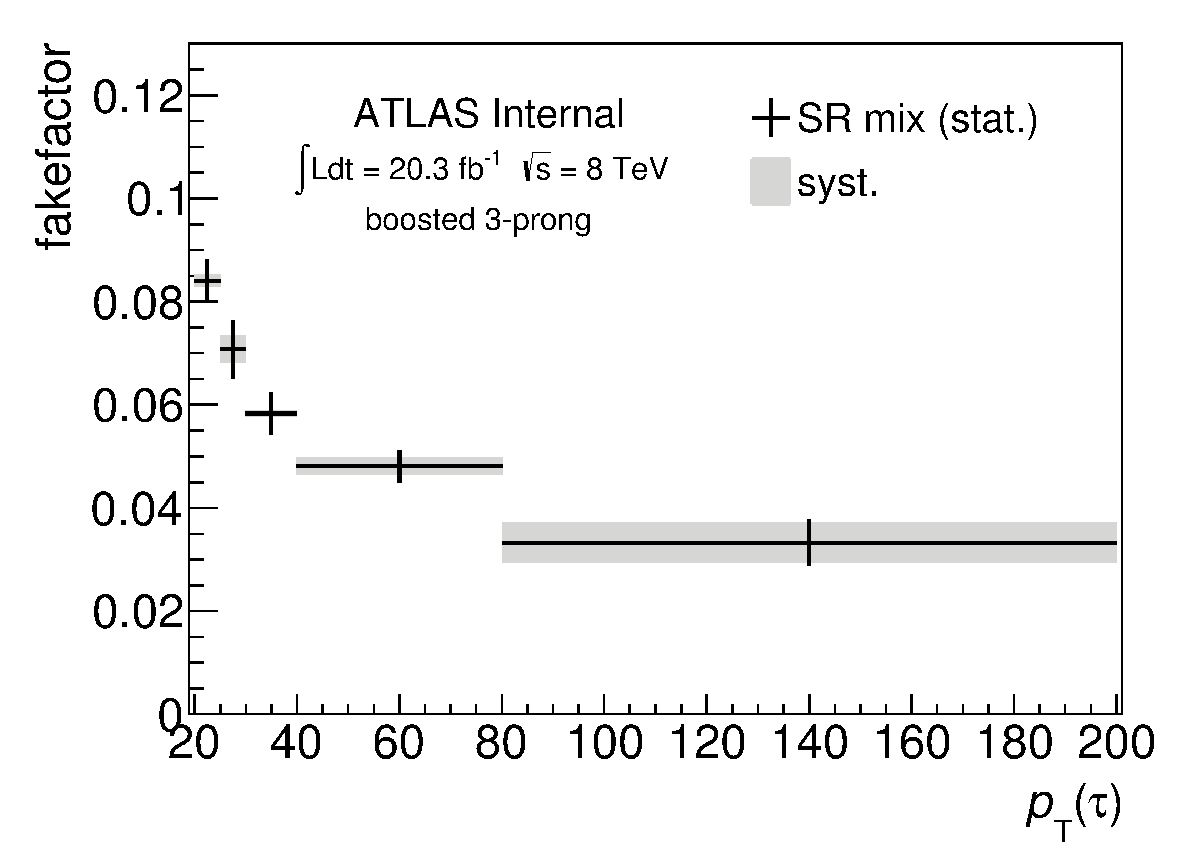
\includegraphics[width=0.48\textwidth]{figures/backgrounds/fakefactor_8TeV_boosted_3p_mix}
  \caption{Variables.}
  \label{fig:backgrounds-fakefactorsboost3p}
\end{figure}

\begin{figure}[tp]
  \centering
  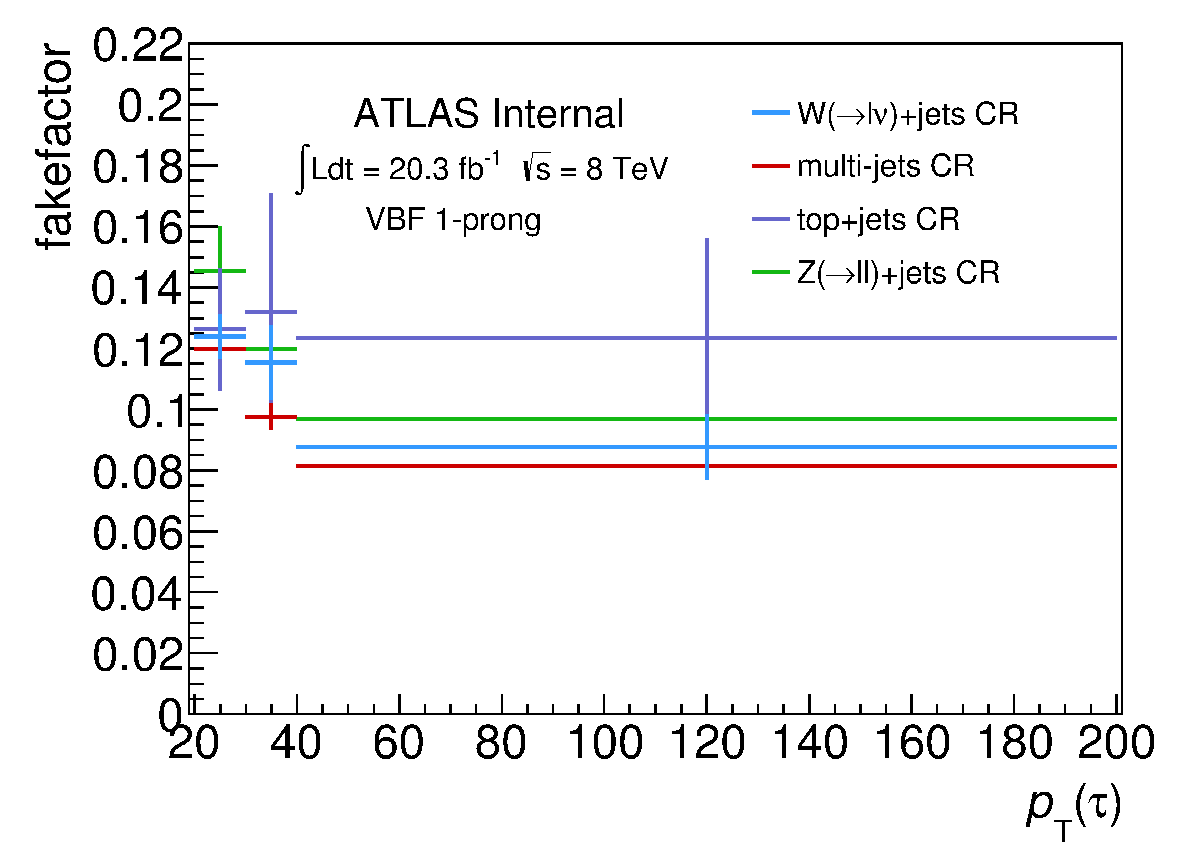
\includegraphics[width=0.48\textwidth]{figures/backgrounds/fakefactor_8TeV_vbf_1p_CRs}
  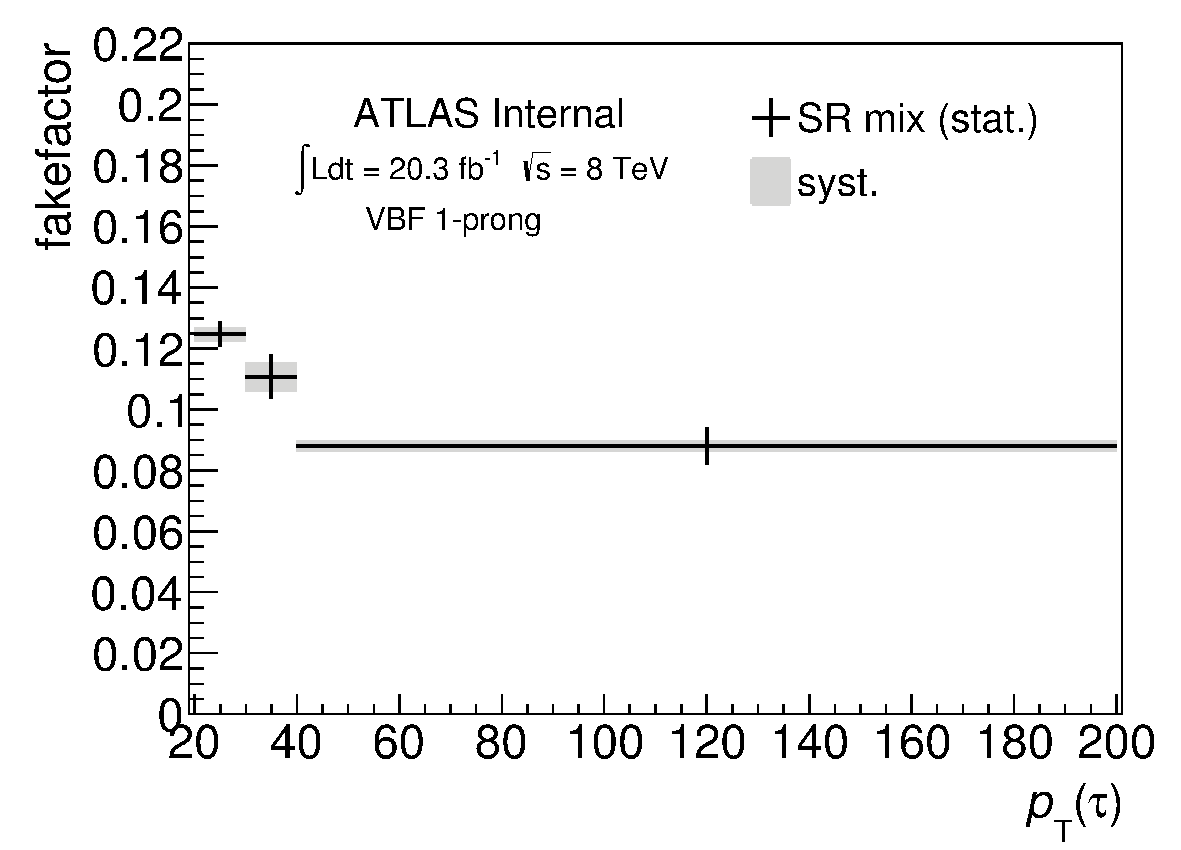
\includegraphics[width=0.48\textwidth]{figures/backgrounds/fakefactor_8TeV_vbf_1p_mix}
  \caption{Variables.}
  \label{fig:backgrounds-fakefactorsVBF1p}
\end{figure}

\begin{figure}[tp]
  \centering
  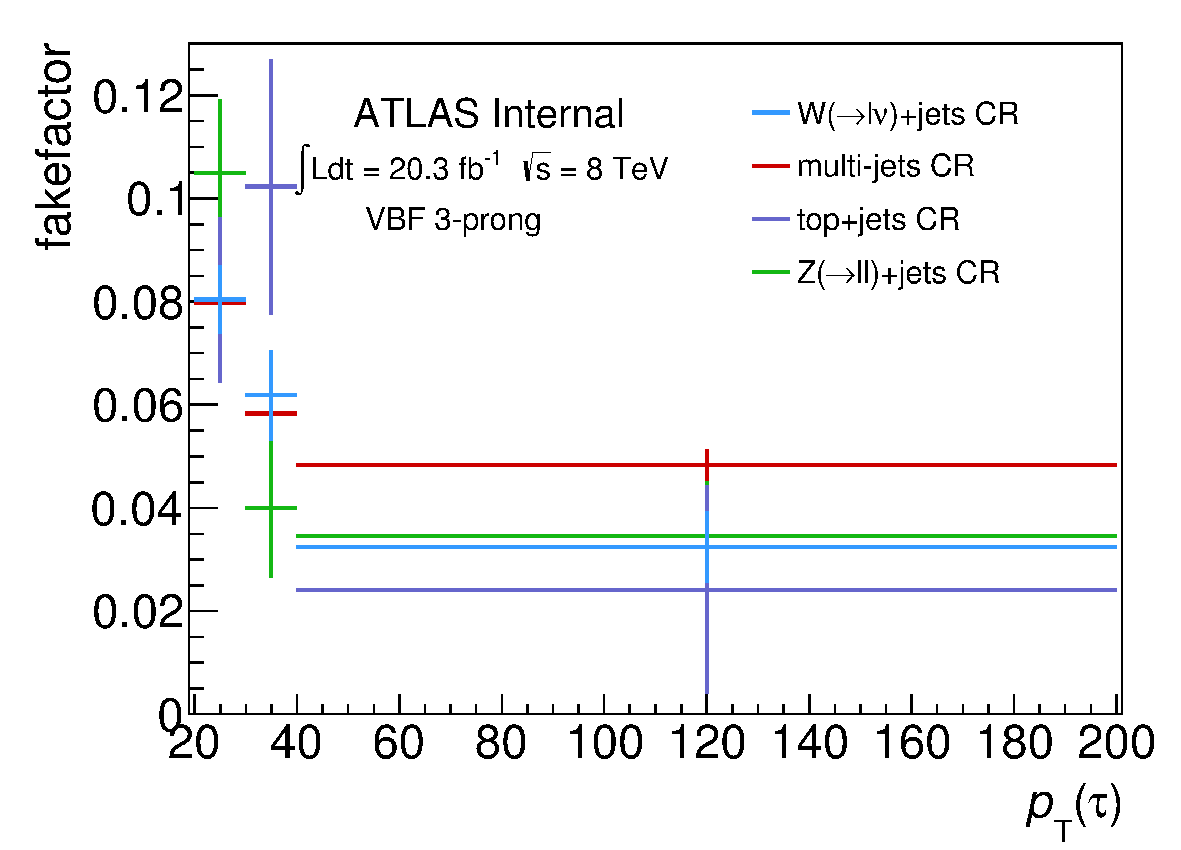
\includegraphics[width=0.48\textwidth]{figures/backgrounds/fakefactor_8TeV_vbf_3p_CRs}
  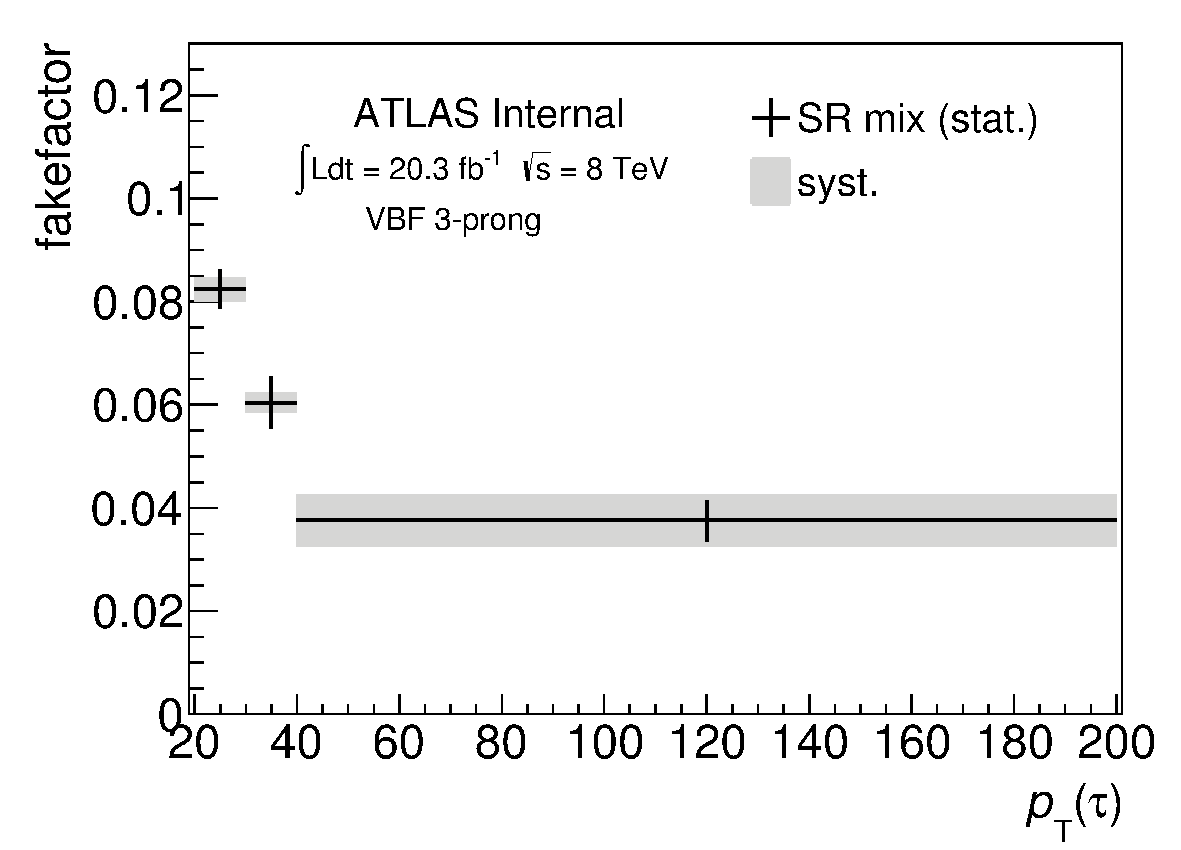
\includegraphics[width=0.48\textwidth]{figures/backgrounds/fakefactor_8TeV_vbf_3p_mix}
  \caption{Variables.}
  \label{fig:backgrounds-fakefactorsVBF3p}
\end{figure}

\clearpage
\begin{figure}[tp]
  \centering
  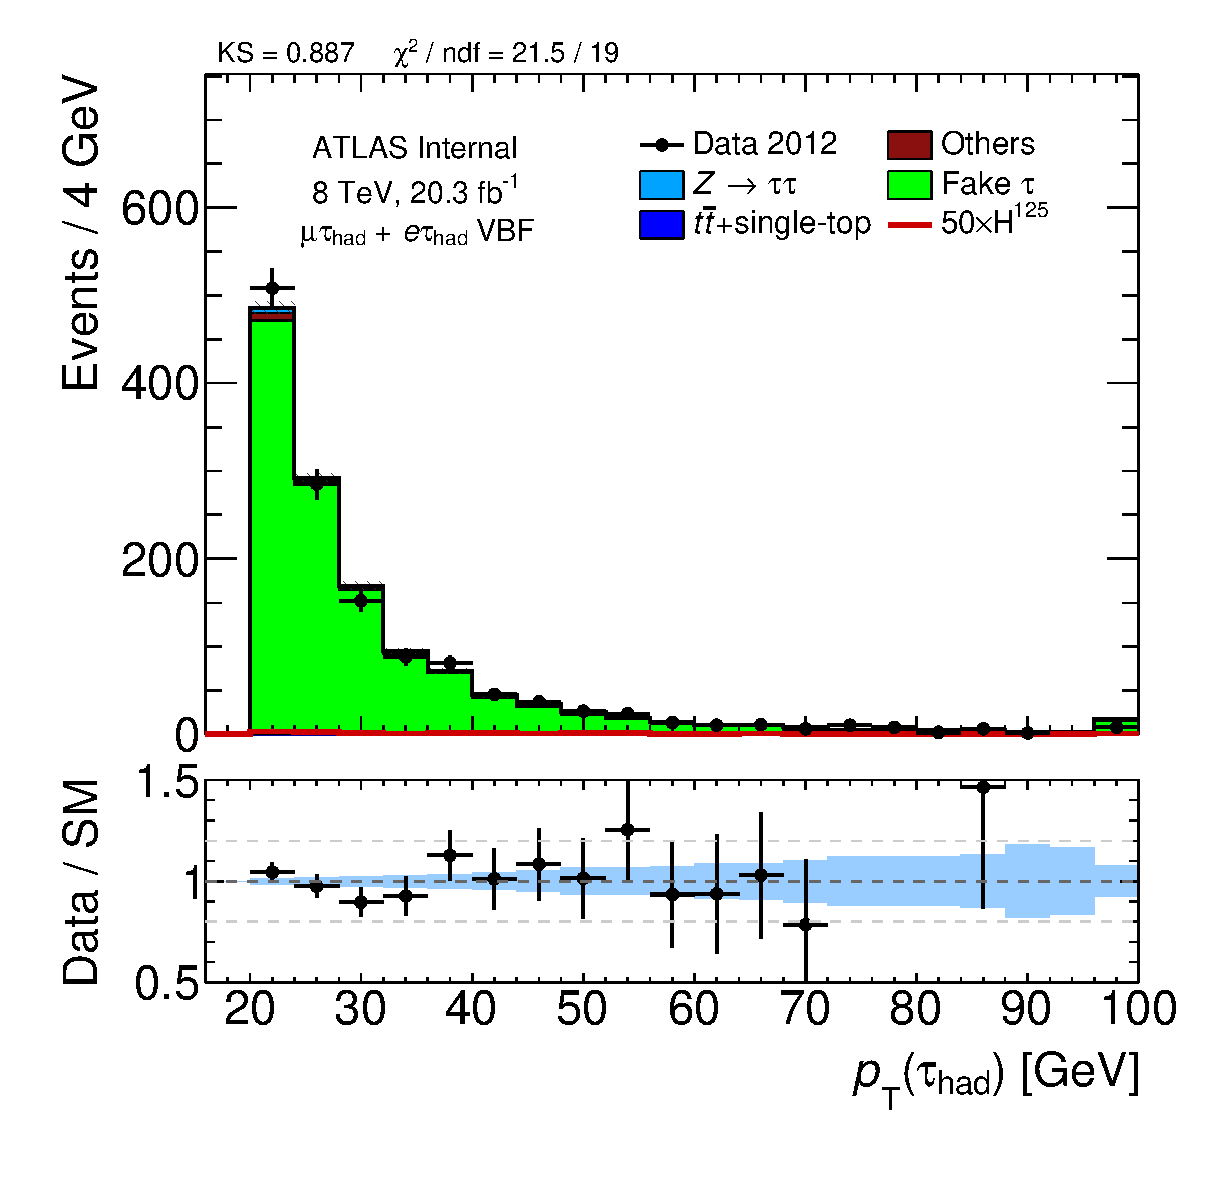
\includegraphics[width=0.32\textwidth]{figures/analysis/vbf-SSXCR/tau-pt}
  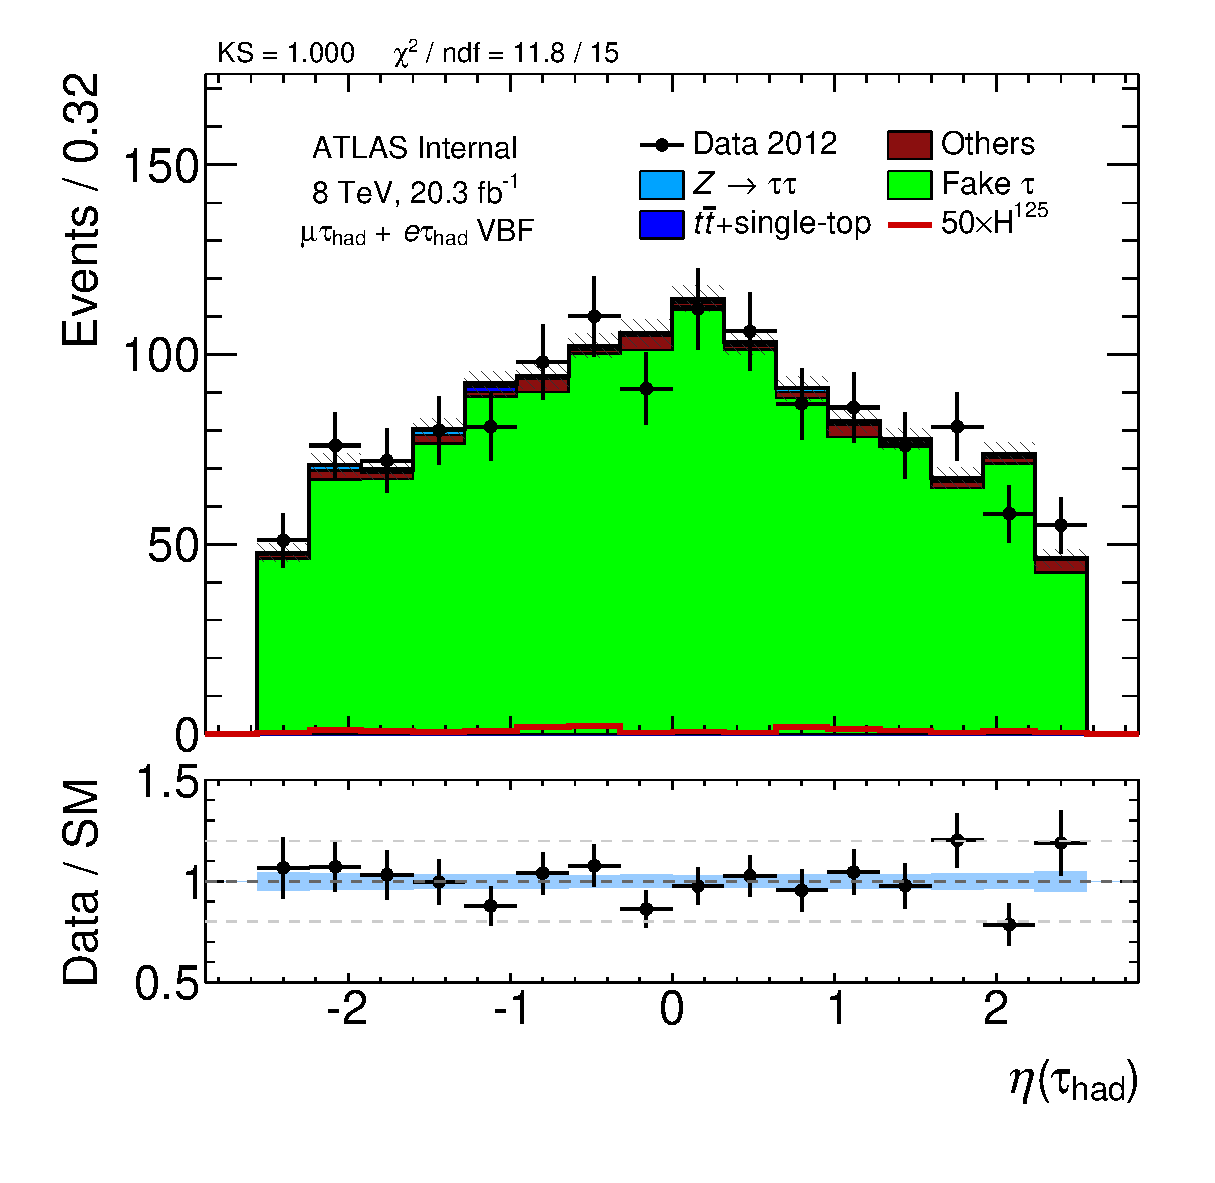
\includegraphics[width=0.32\textwidth]{figures/analysis/vbf-SSXCR/tau-eta}
  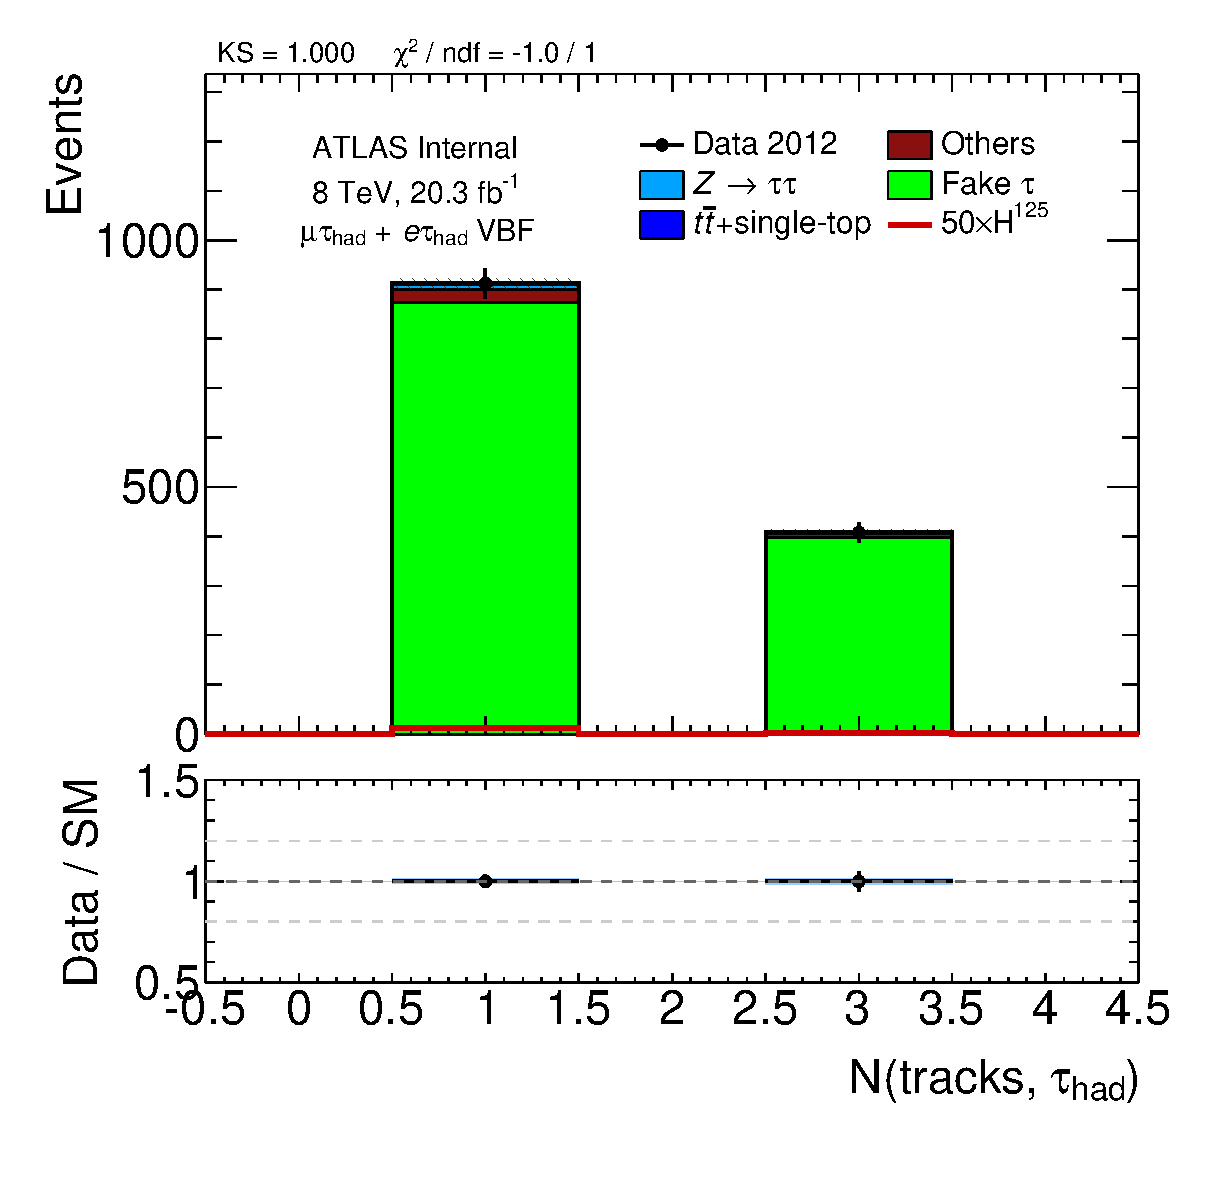
\includegraphics[width=0.32\textwidth]{figures/analysis/vbf-SSXCR/tau-numTrack}
  % --------------
  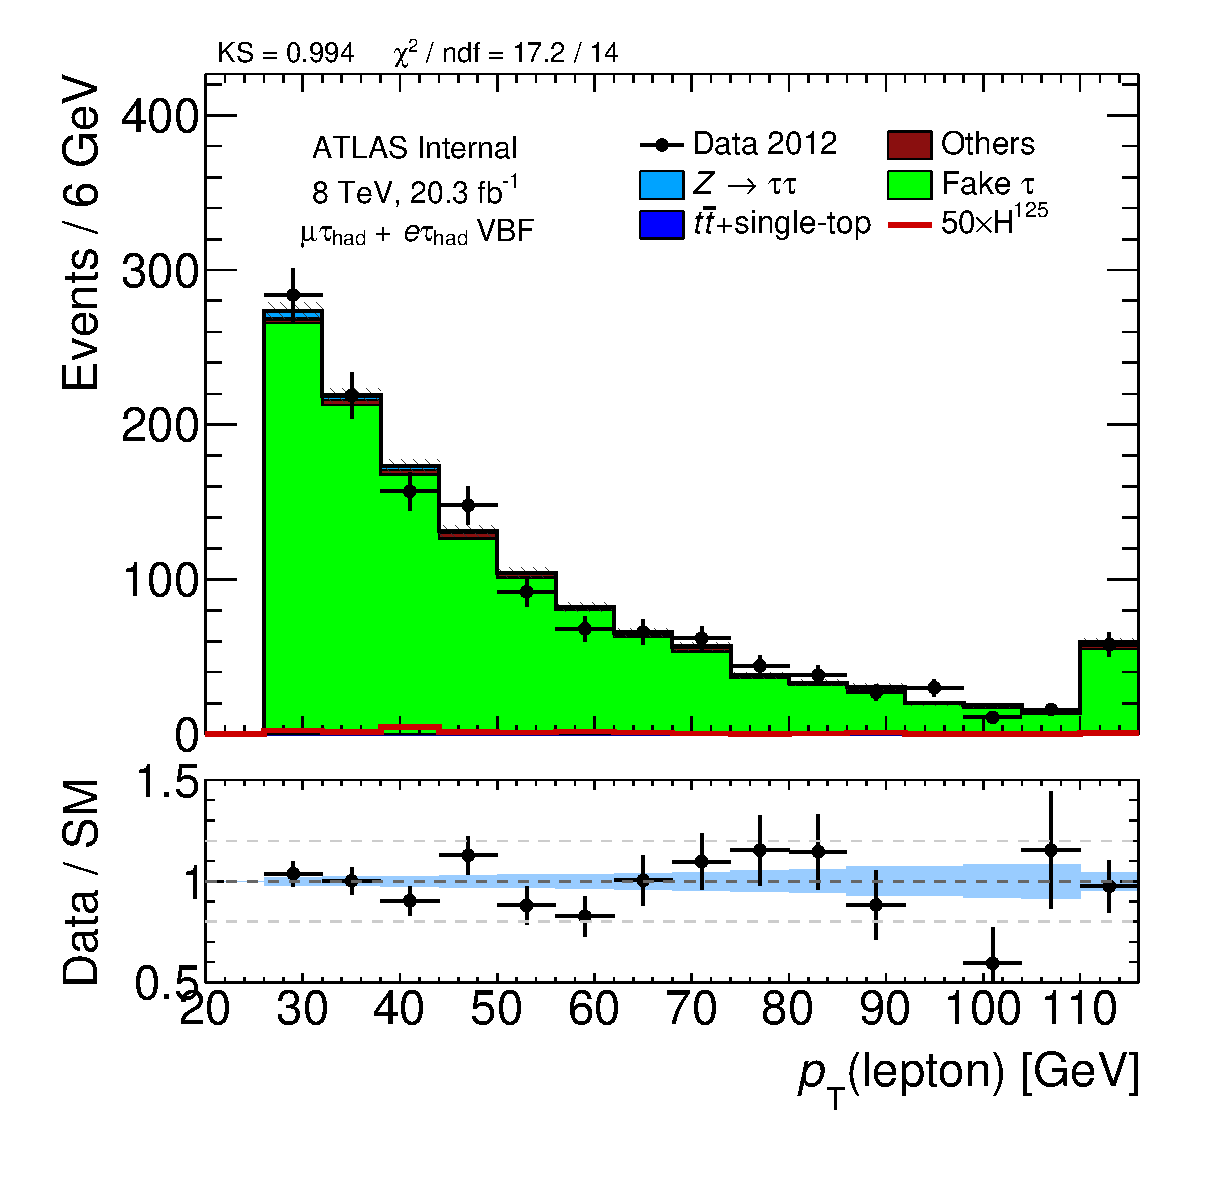
\includegraphics[width=0.32\textwidth]{figures/analysis/vbf-SSXCR/lep-pt-hi}
  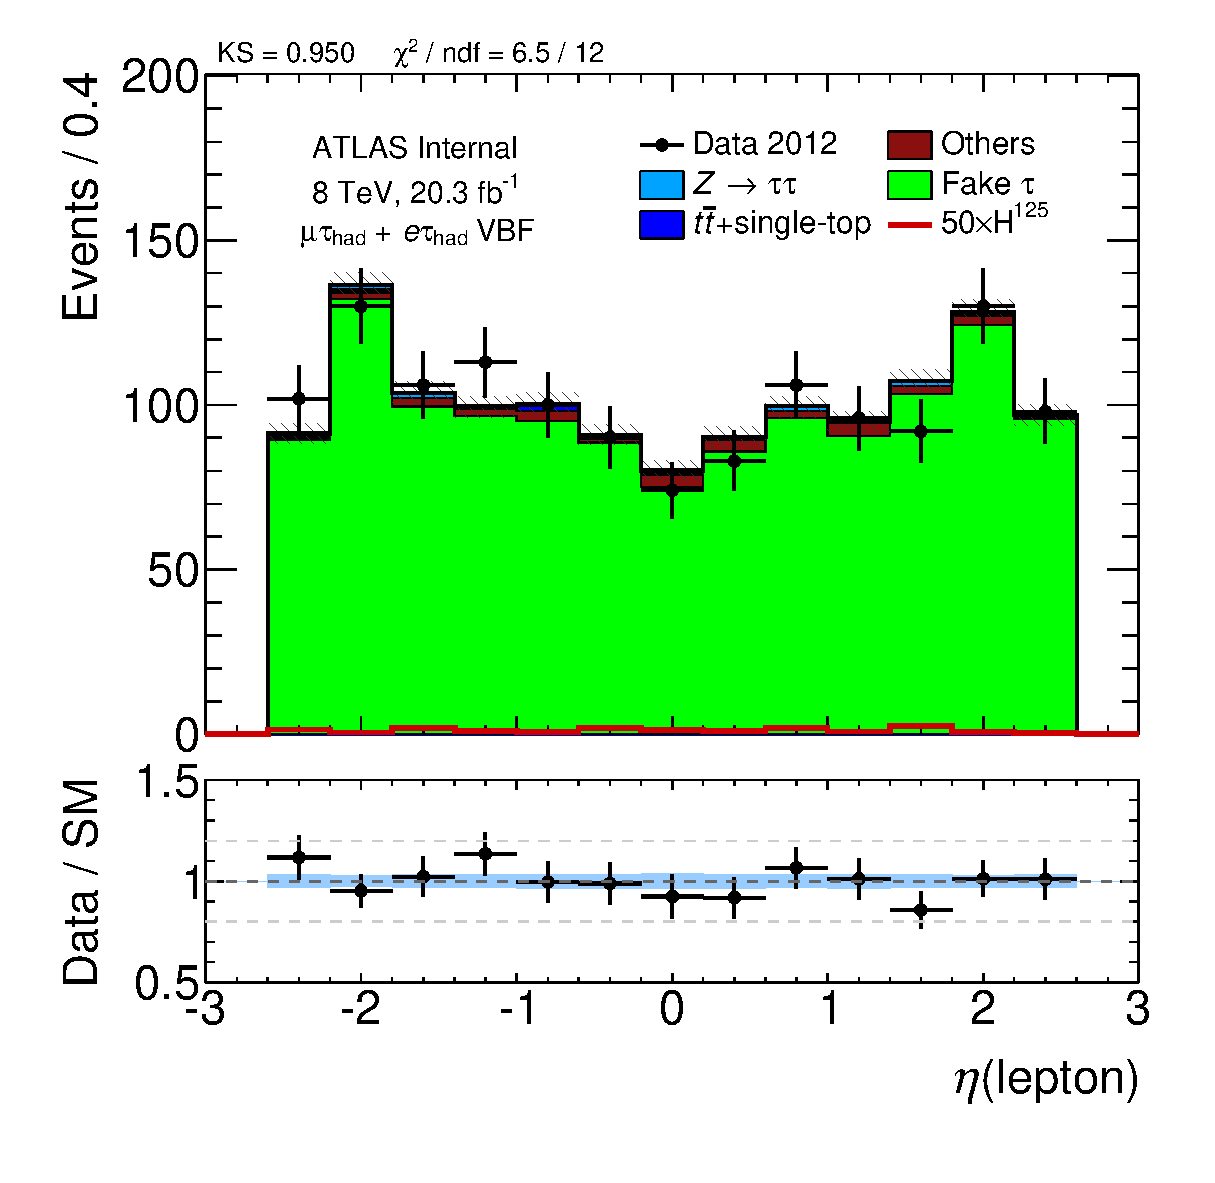
\includegraphics[width=0.32\textwidth]{figures/analysis/vbf-SSXCR/lep-eta}
  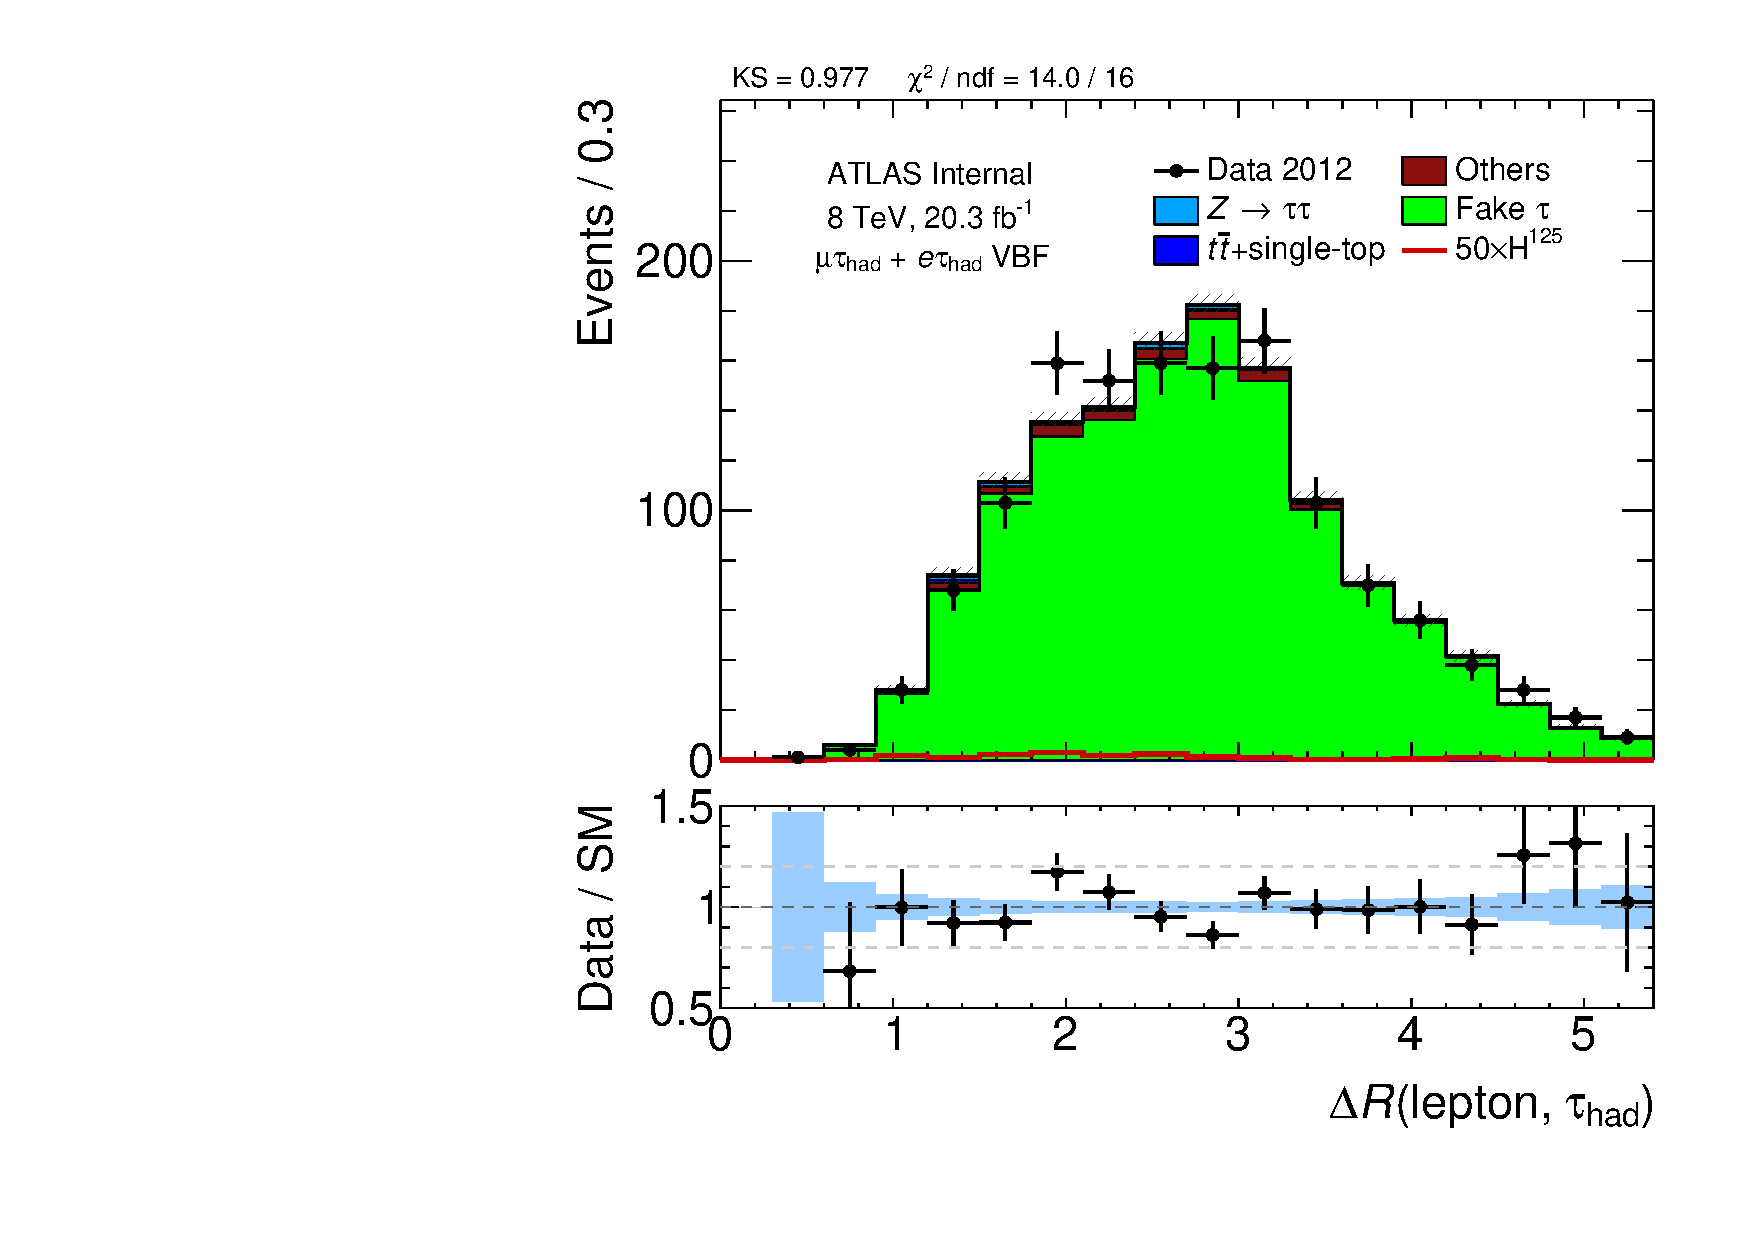
\includegraphics[width=0.32\textwidth]{figures/analysis/vbf-SSXCR/taulep-dR}
  % --------------
  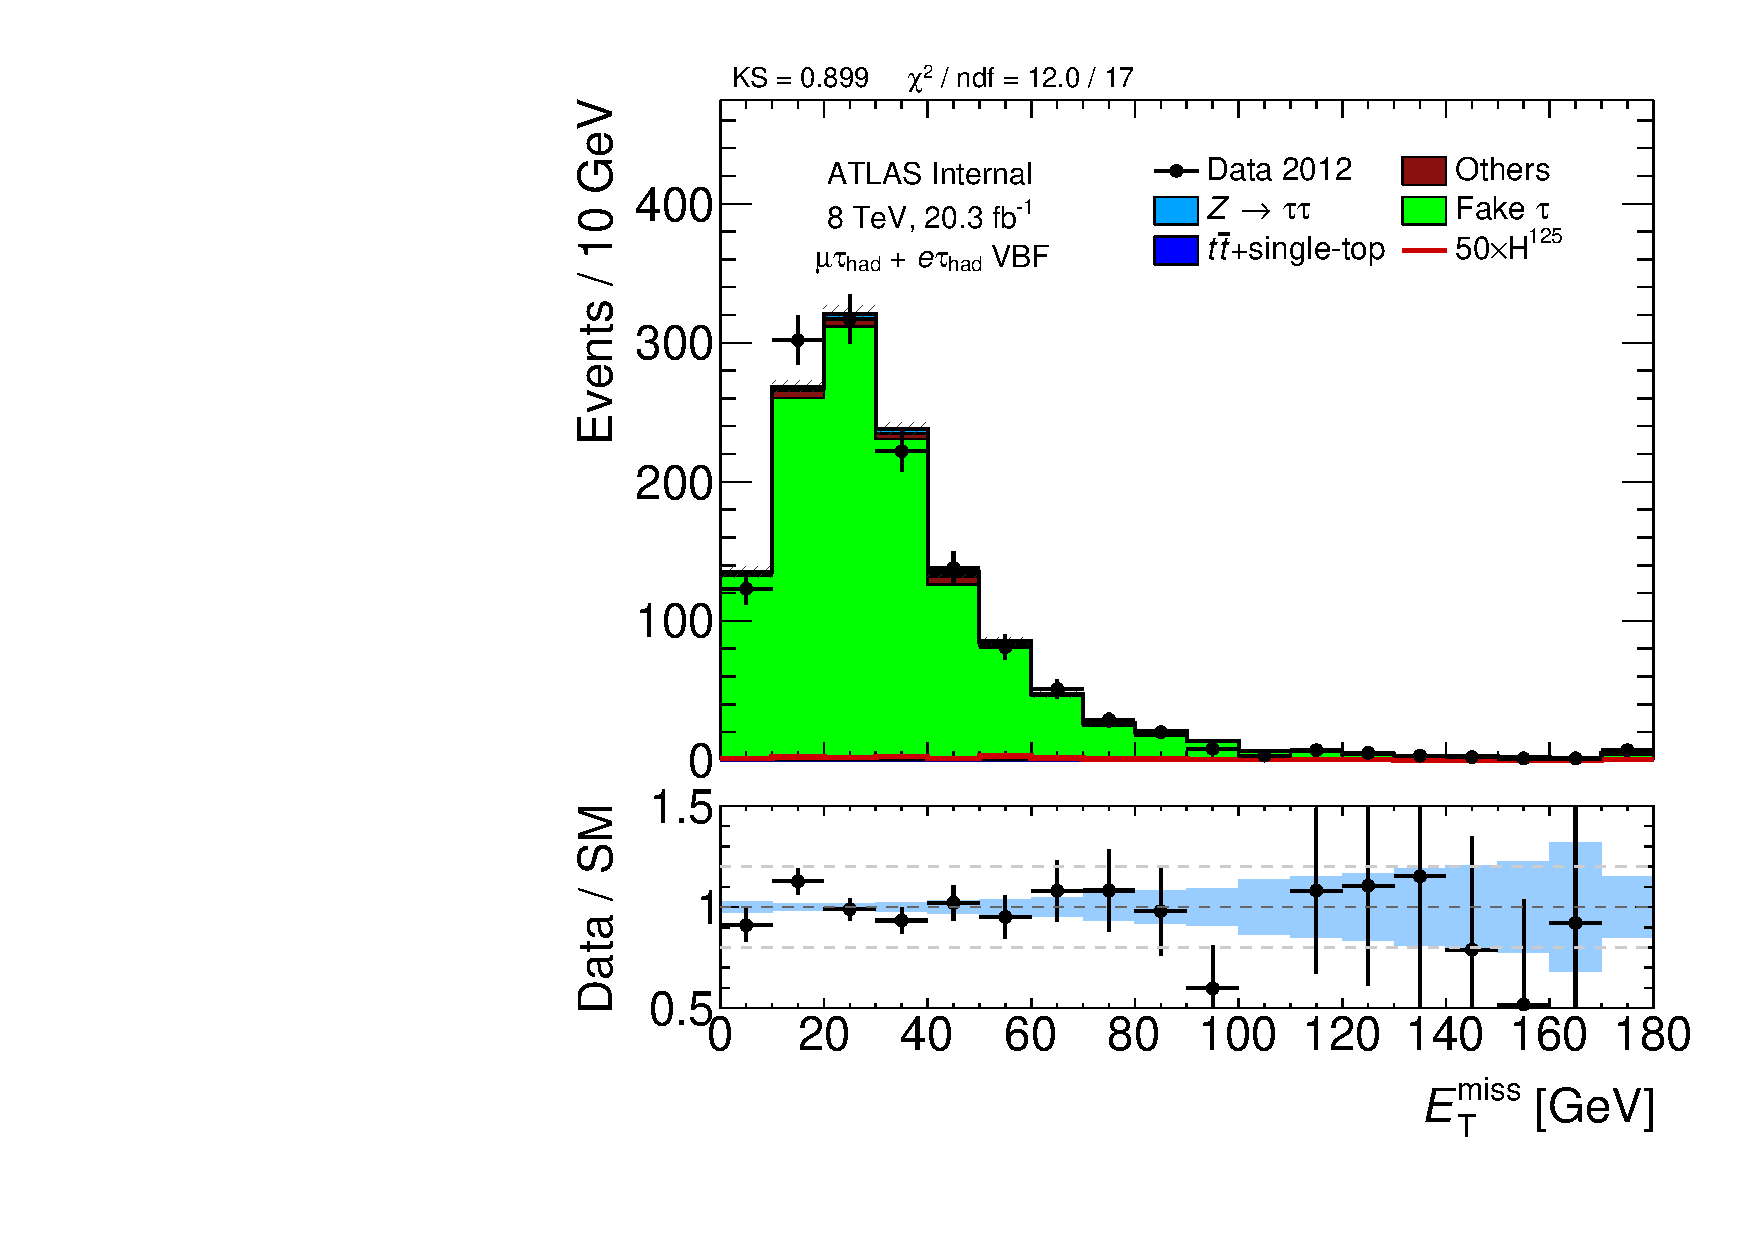
\includegraphics[width=0.32\textwidth]{figures/analysis/vbf-SSXCR/met-pt-hi}
  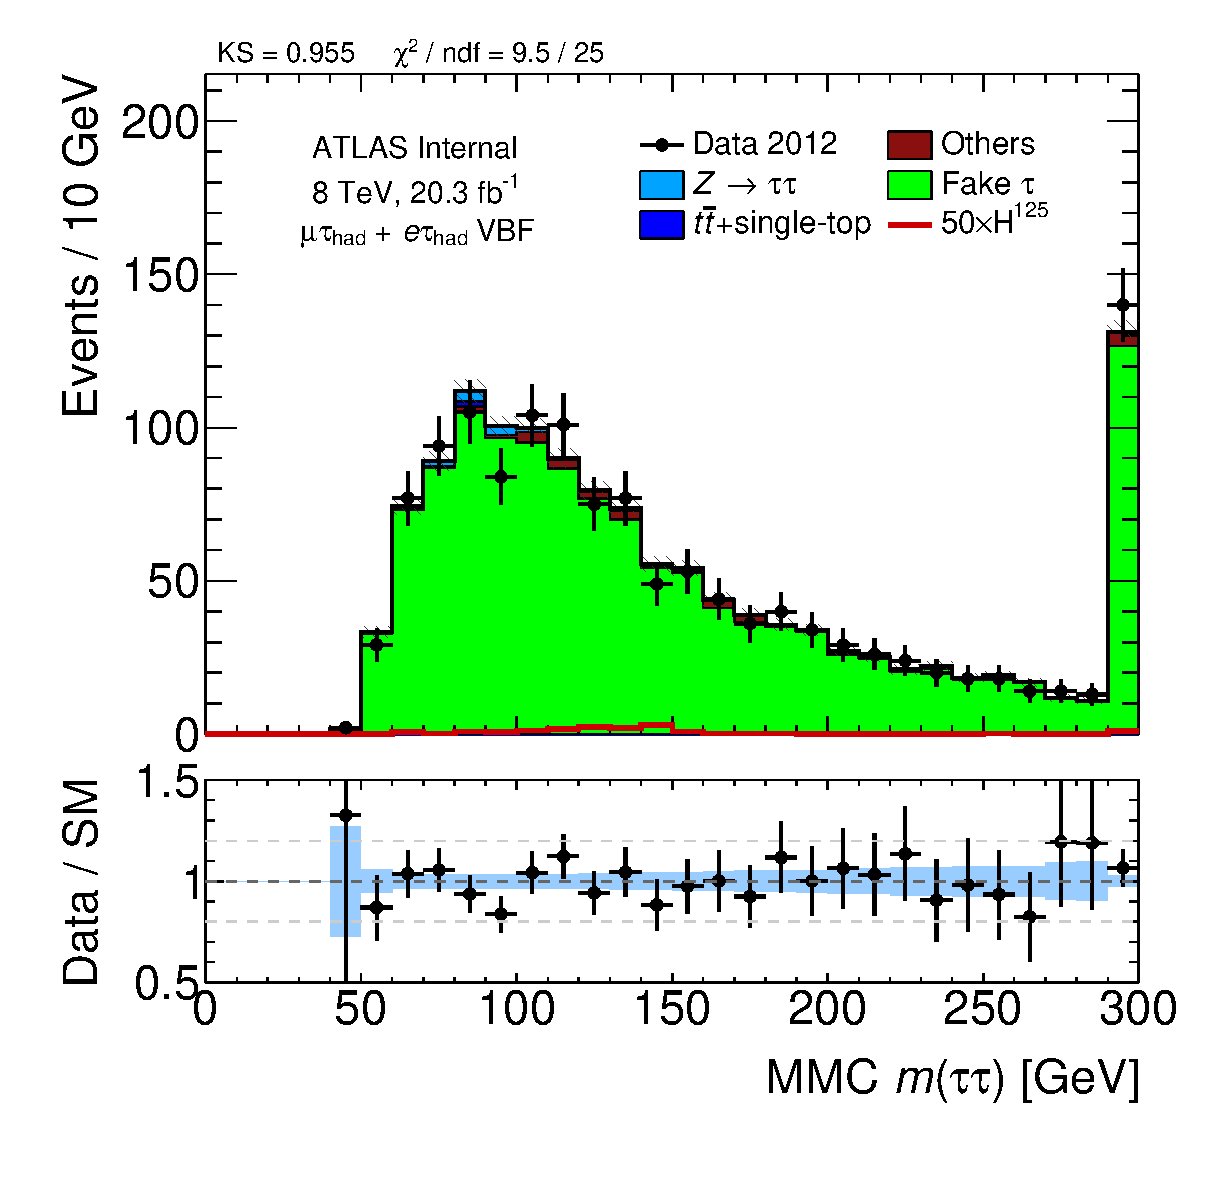
\includegraphics[width=0.32\textwidth]{figures/analysis/vbf-SSXCR/mMMC}
  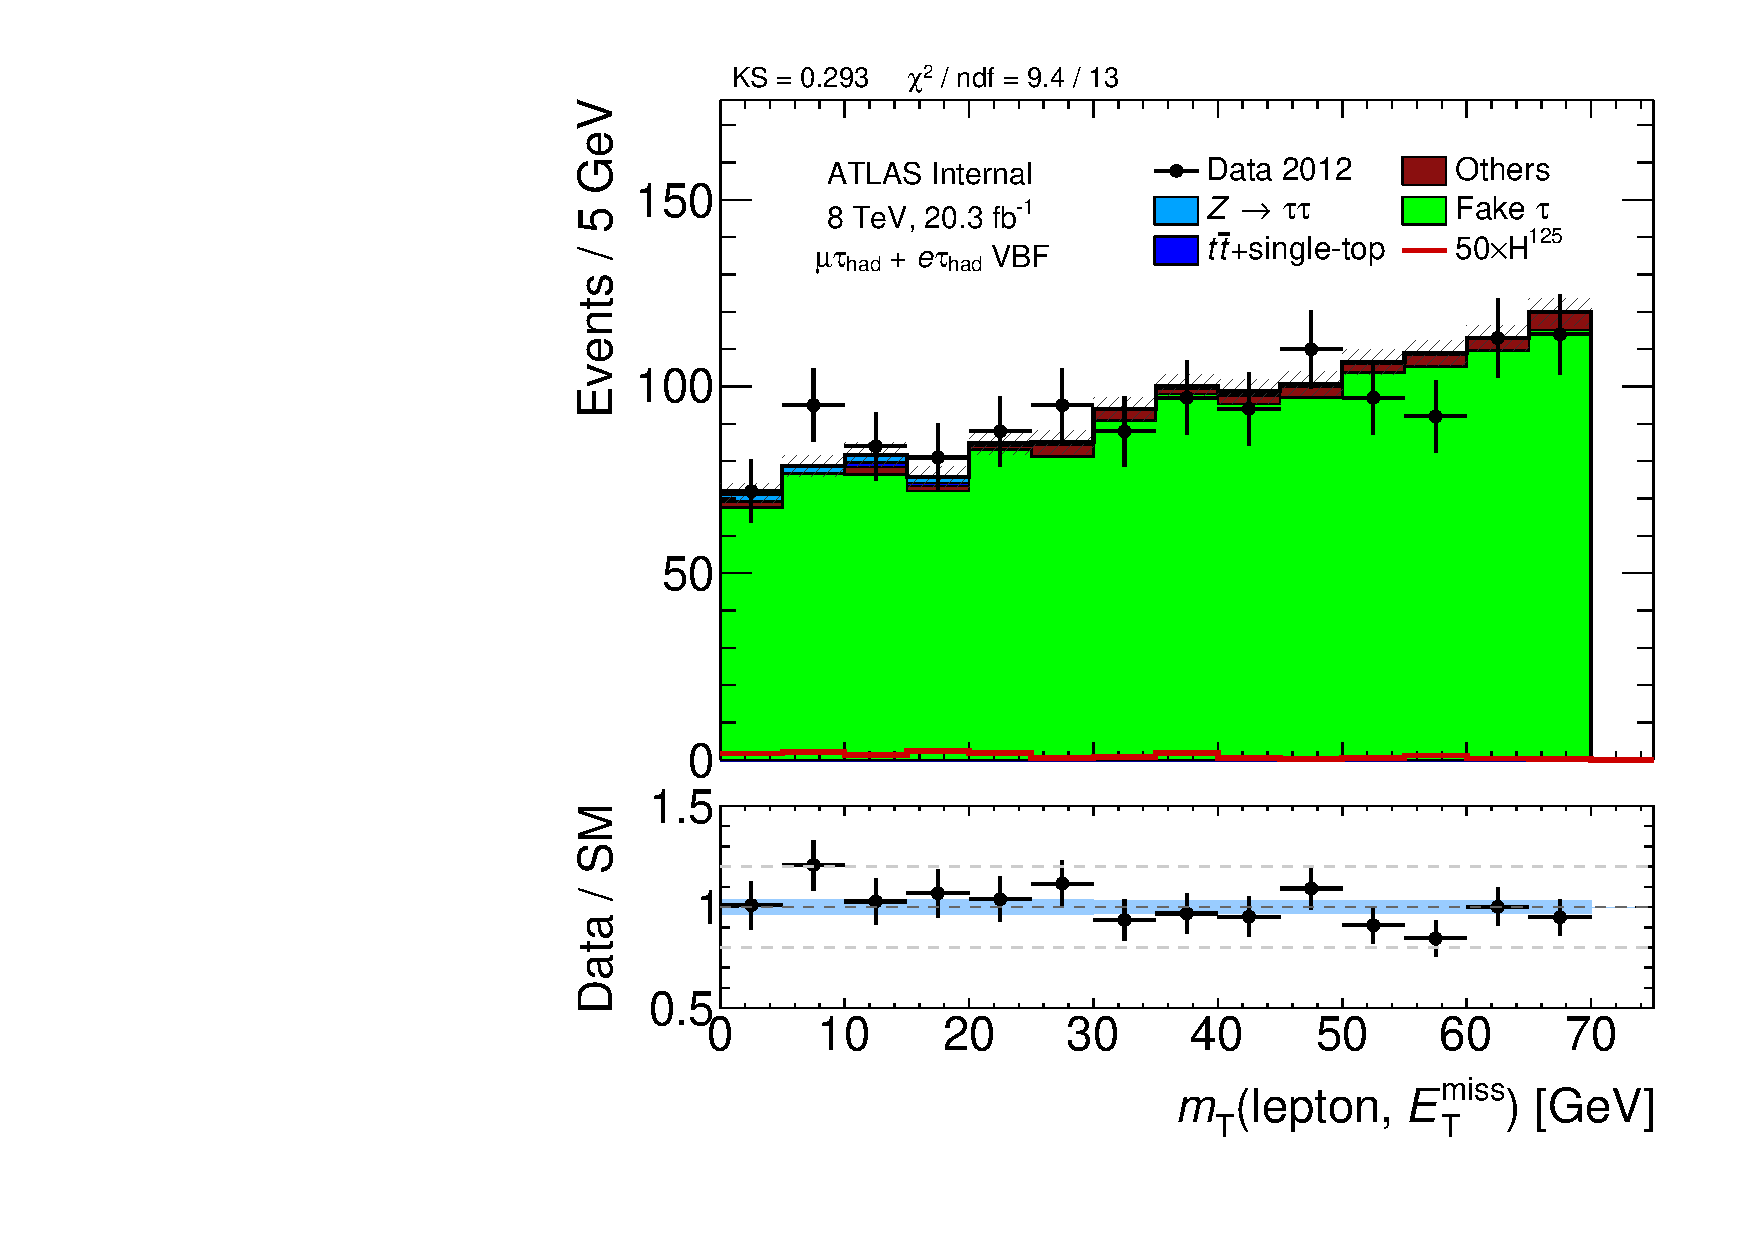
\includegraphics[width=0.32\textwidth]{figures/analysis/vbf-SSXCR/mT}
  % --------------
  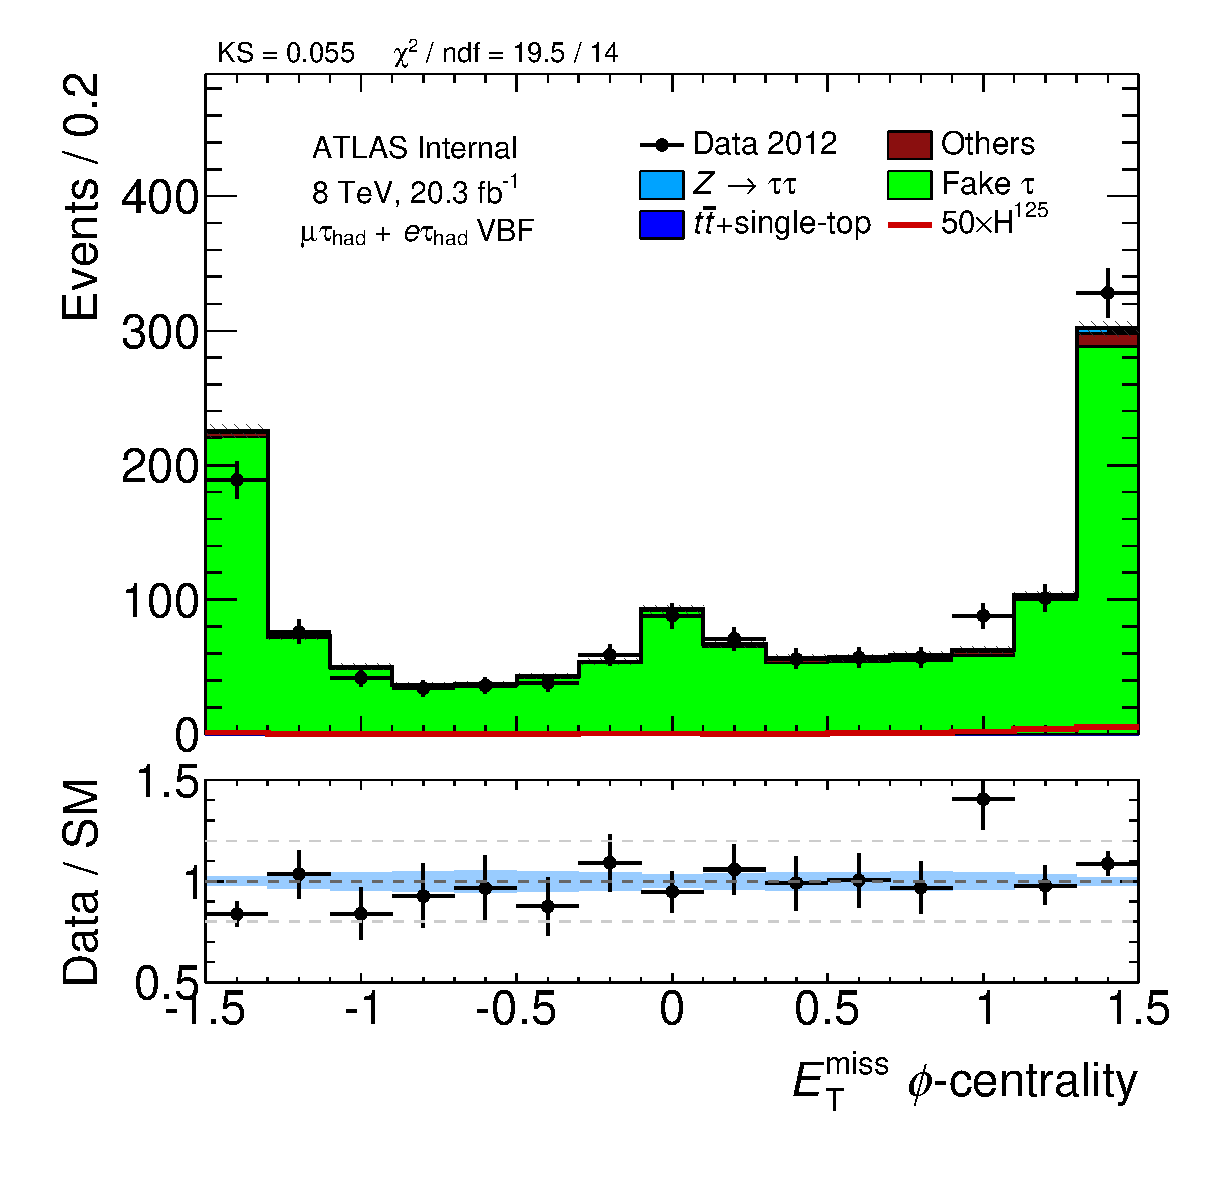
\includegraphics[width=0.32\textwidth]{figures/analysis/vbf-SSXCR/met-phi-centrality}
  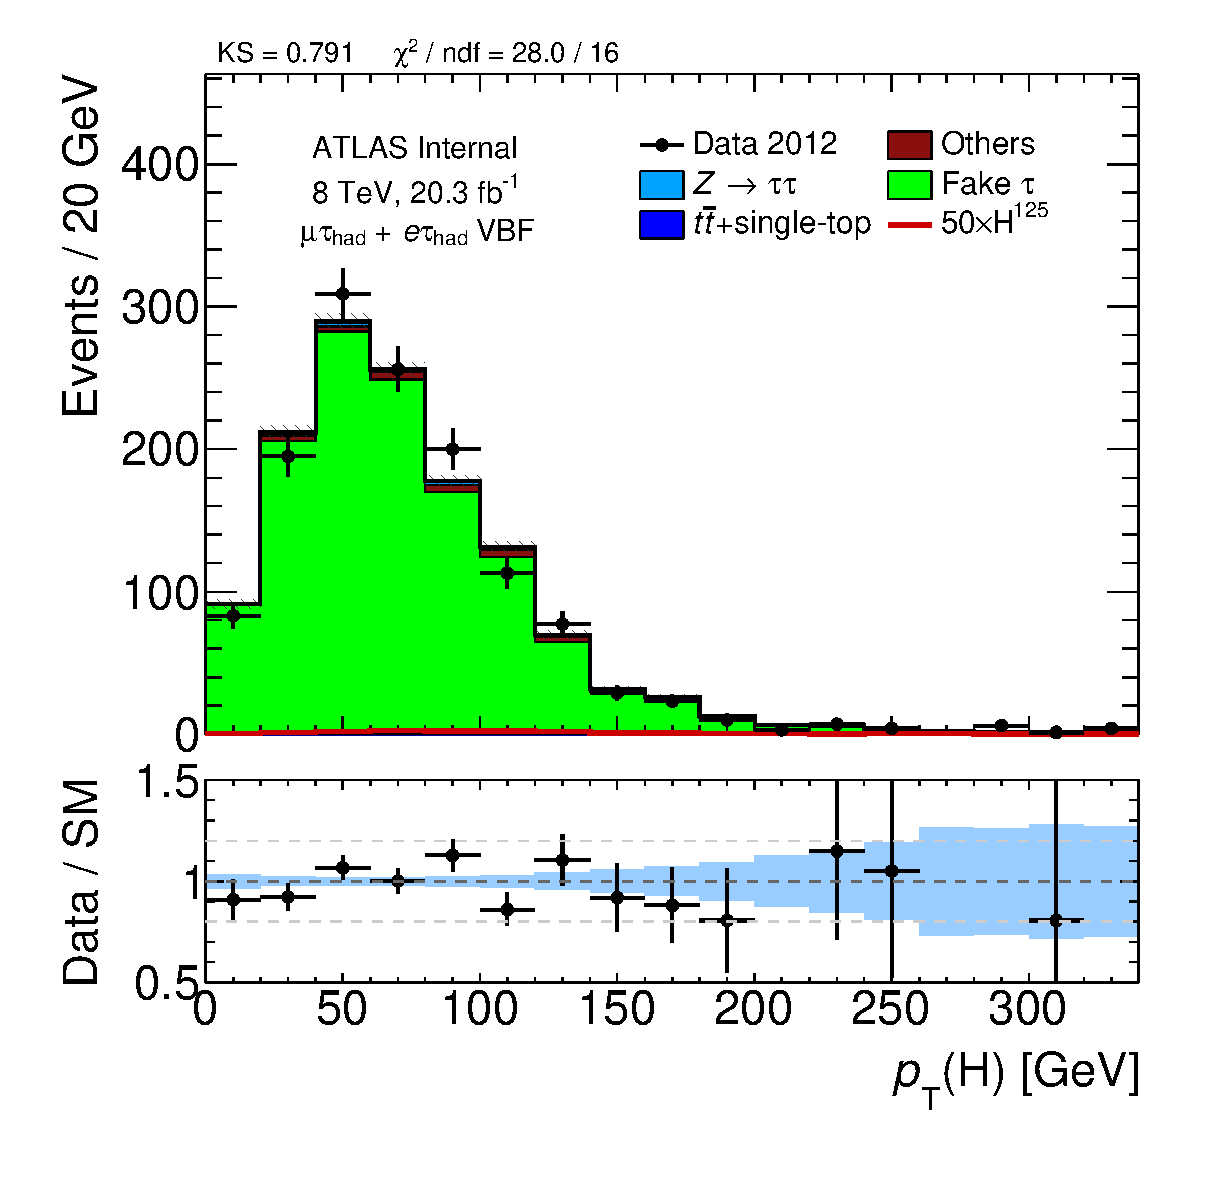
\includegraphics[width=0.32\textwidth]{figures/analysis/vbf-SSXCR/H-pt-hi}
  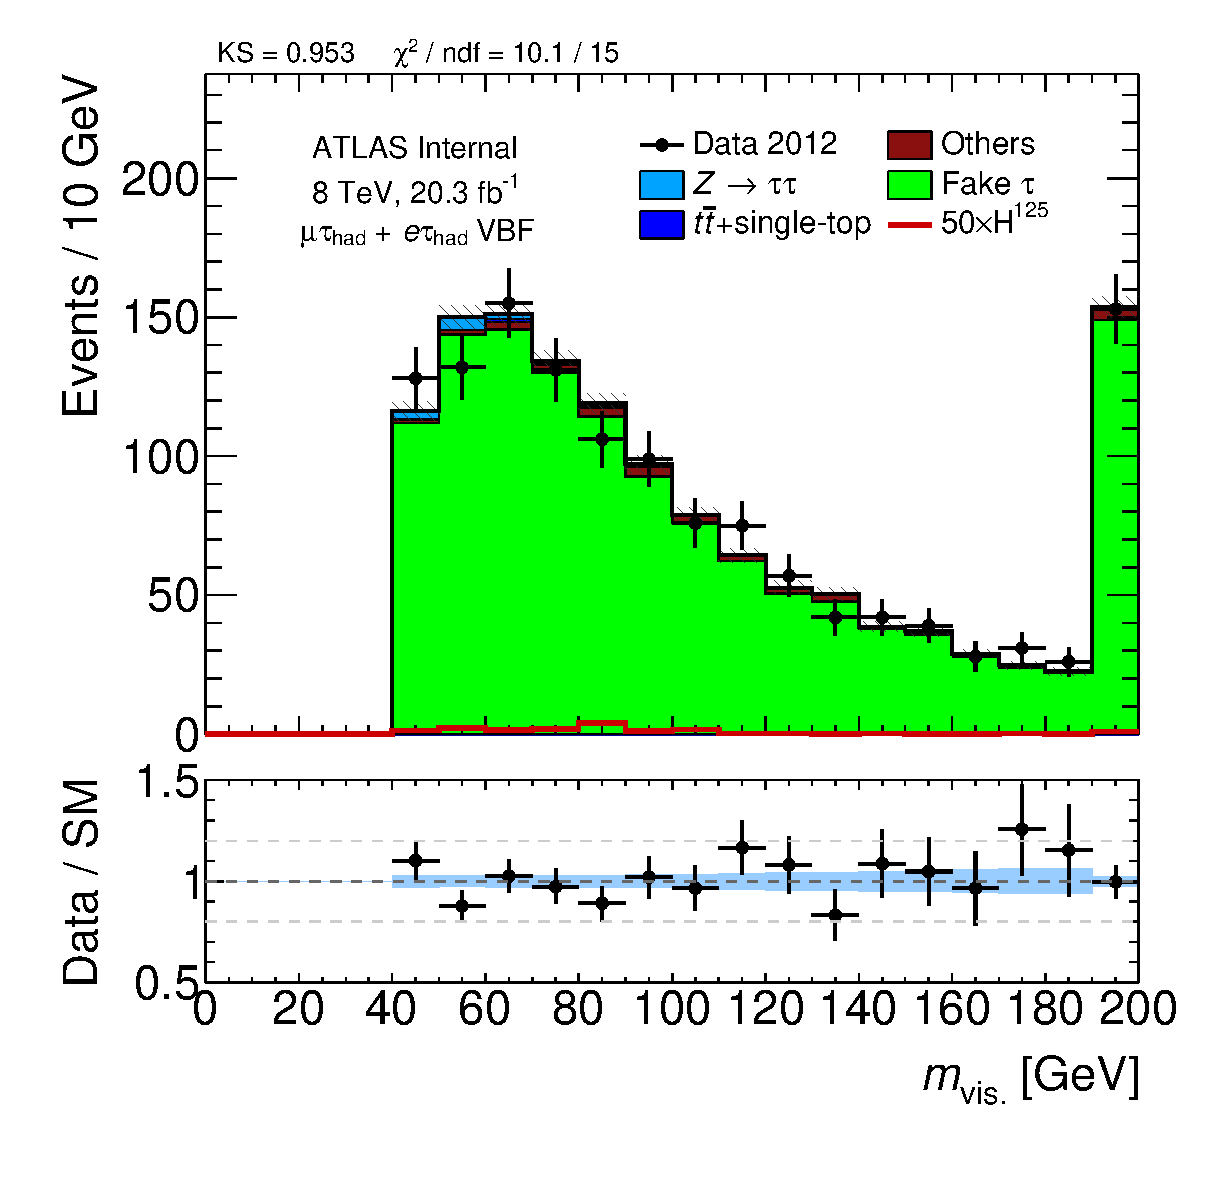
\includegraphics[width=0.32\textwidth]{figures/analysis/vbf-SSXCR/mvis}
  \caption{Variables.}
  \label{fig:backgrounds-SSXCR-taus}
\end{figure}

\begin{figure}[tp]
  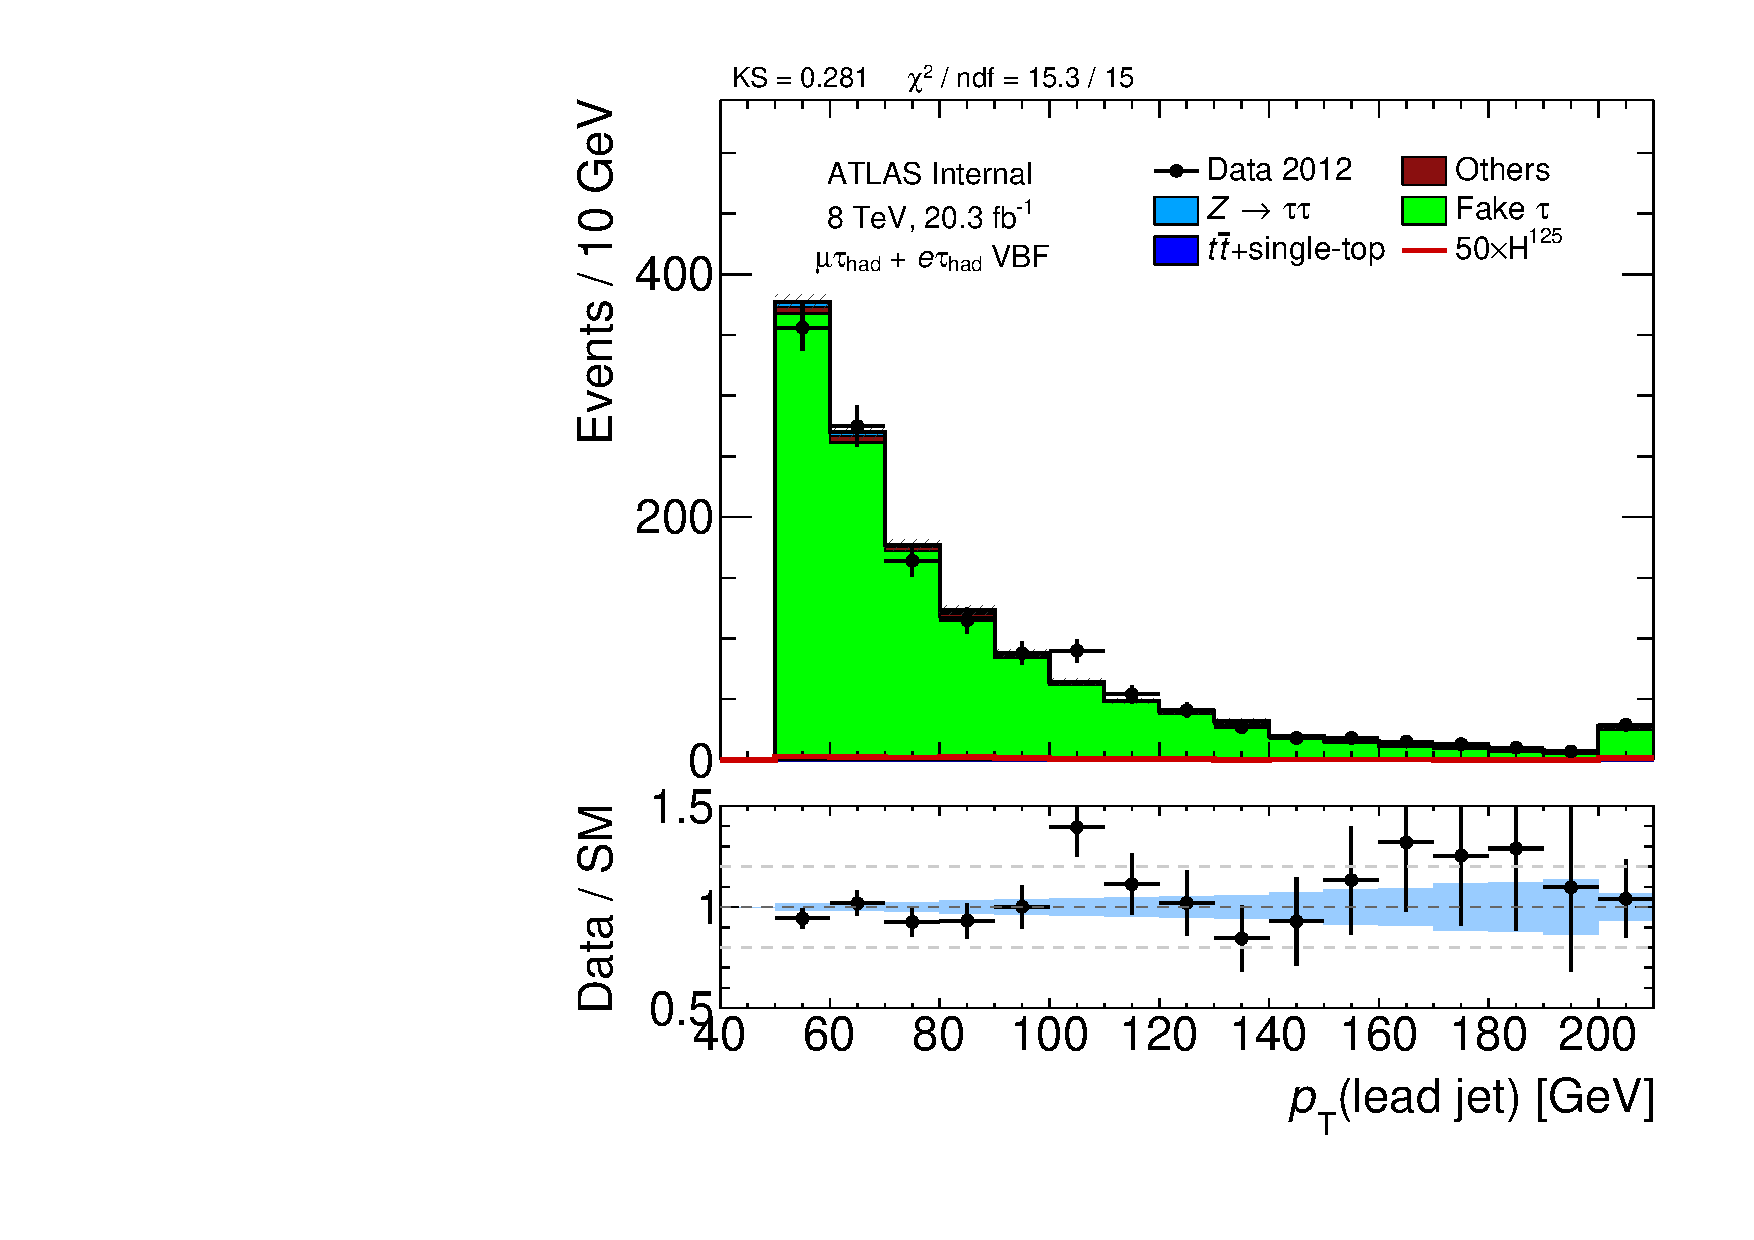
\includegraphics[width=0.32\textwidth]{figures/analysis/vbf-SSXCR/jet-1-pt}
  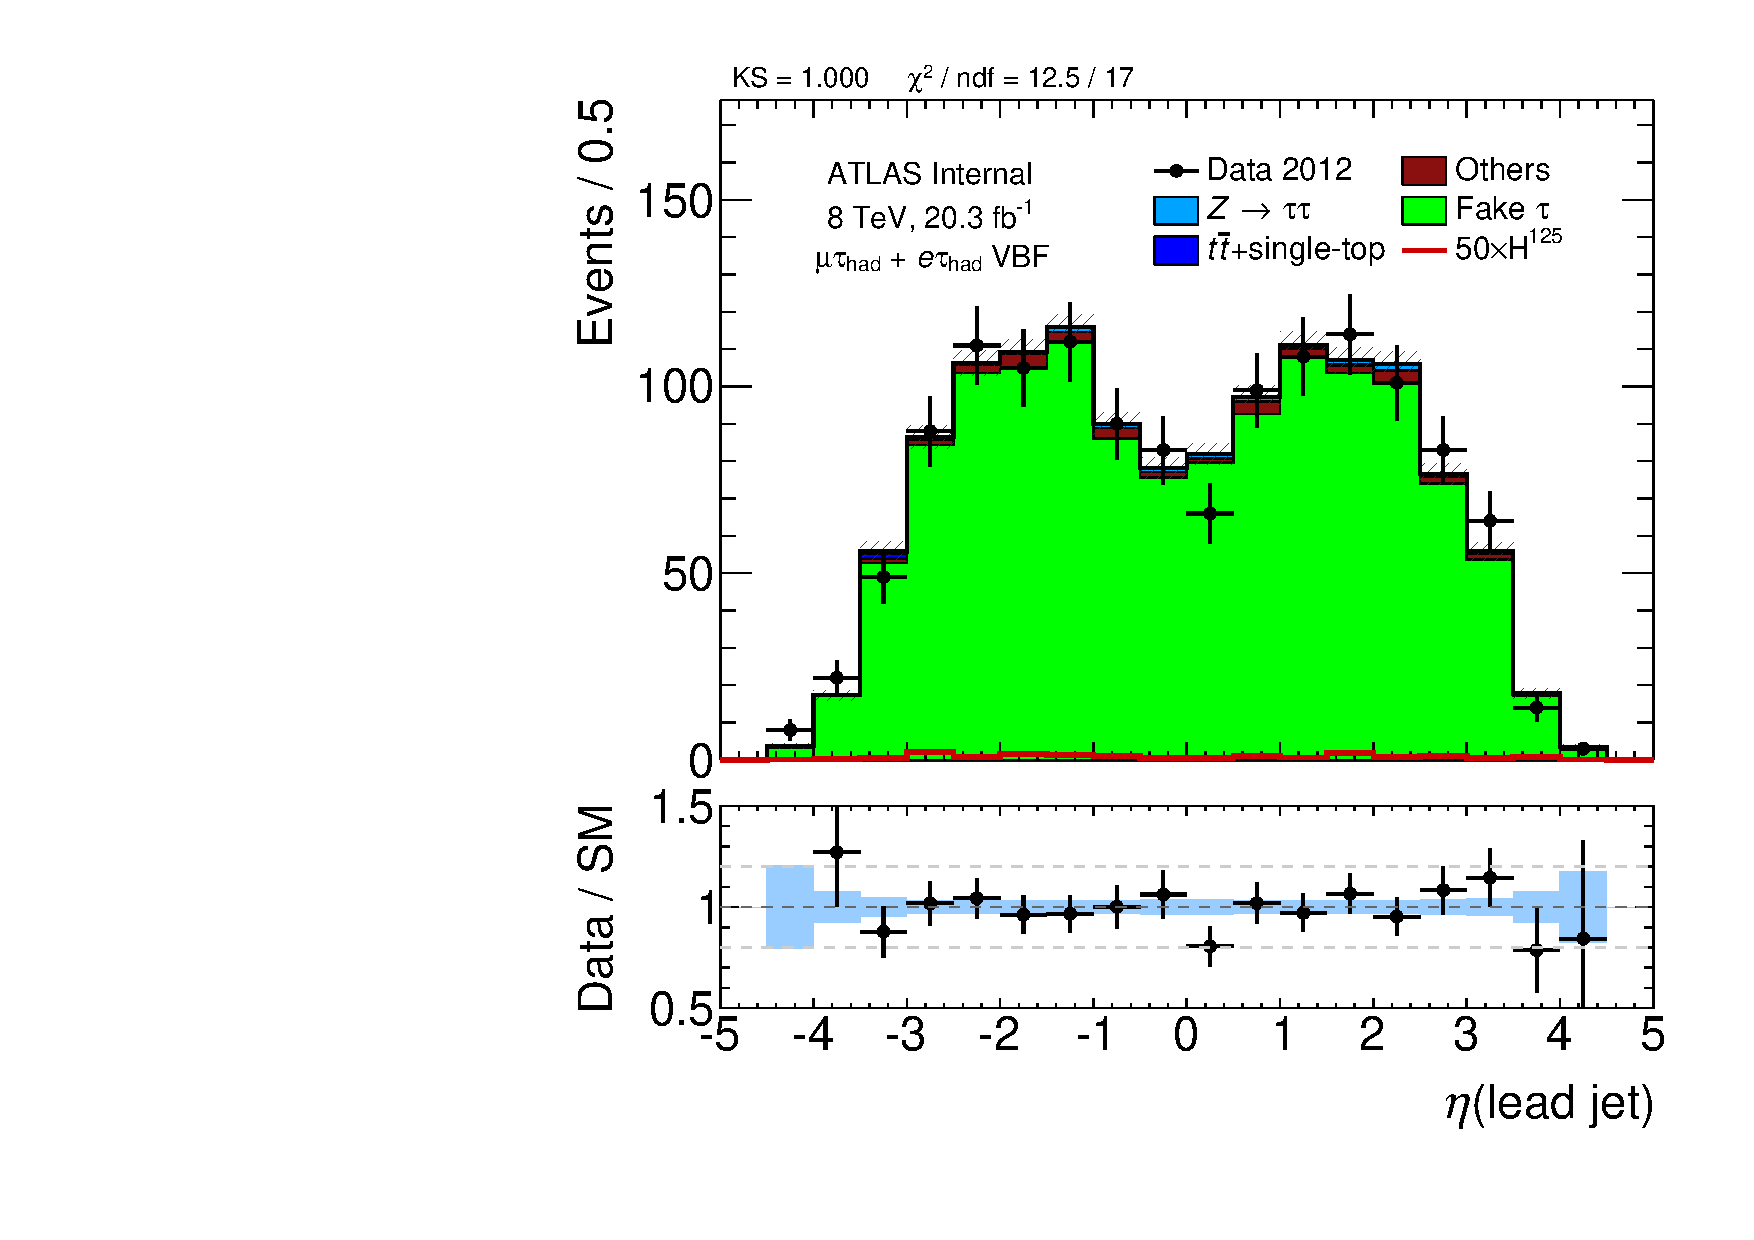
\includegraphics[width=0.32\textwidth]{figures/analysis/vbf-SSXCR/jet-1-eta}
  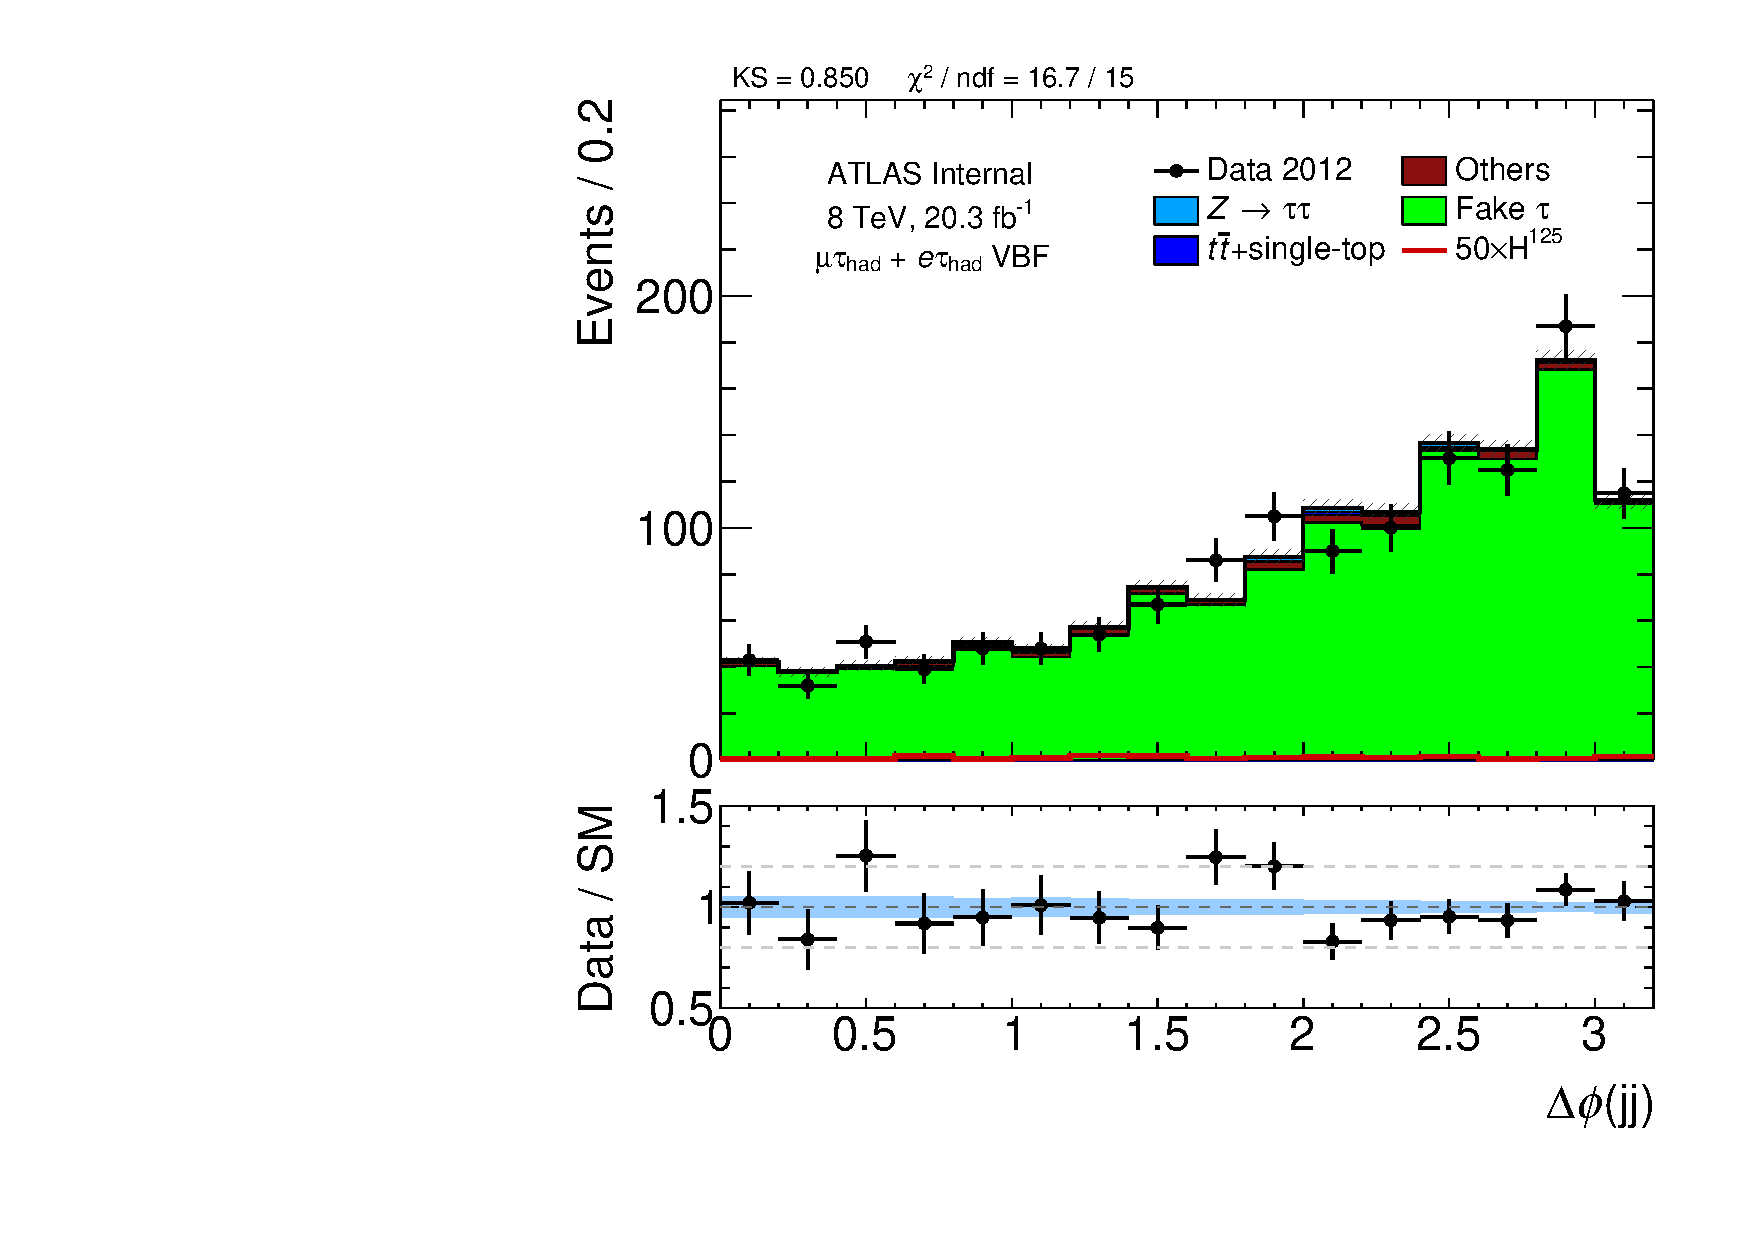
\includegraphics[width=0.32\textwidth]{figures/analysis/vbf-SSXCR/jets-dphi}
  % --------------
  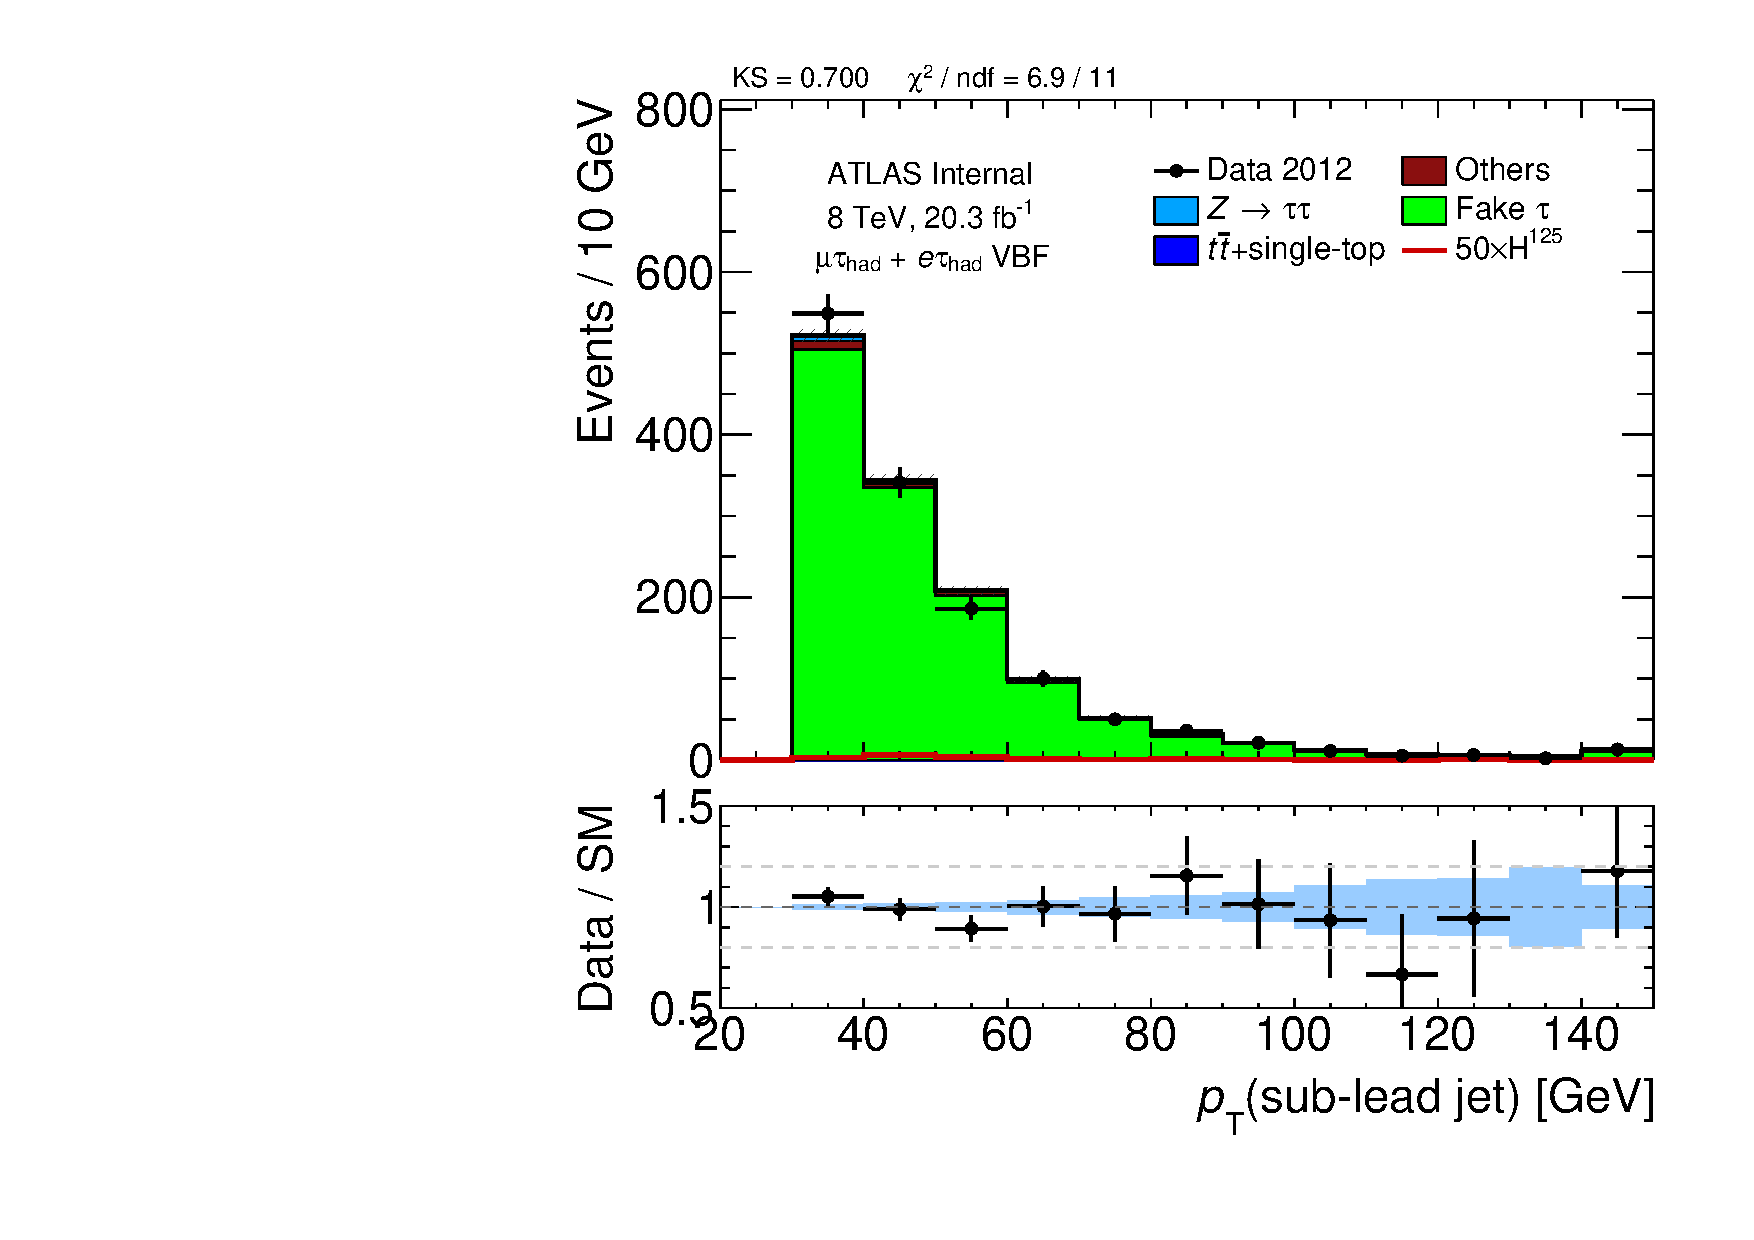
\includegraphics[width=0.32\textwidth]{figures/analysis/vbf-SSXCR/jet-2-pt}
  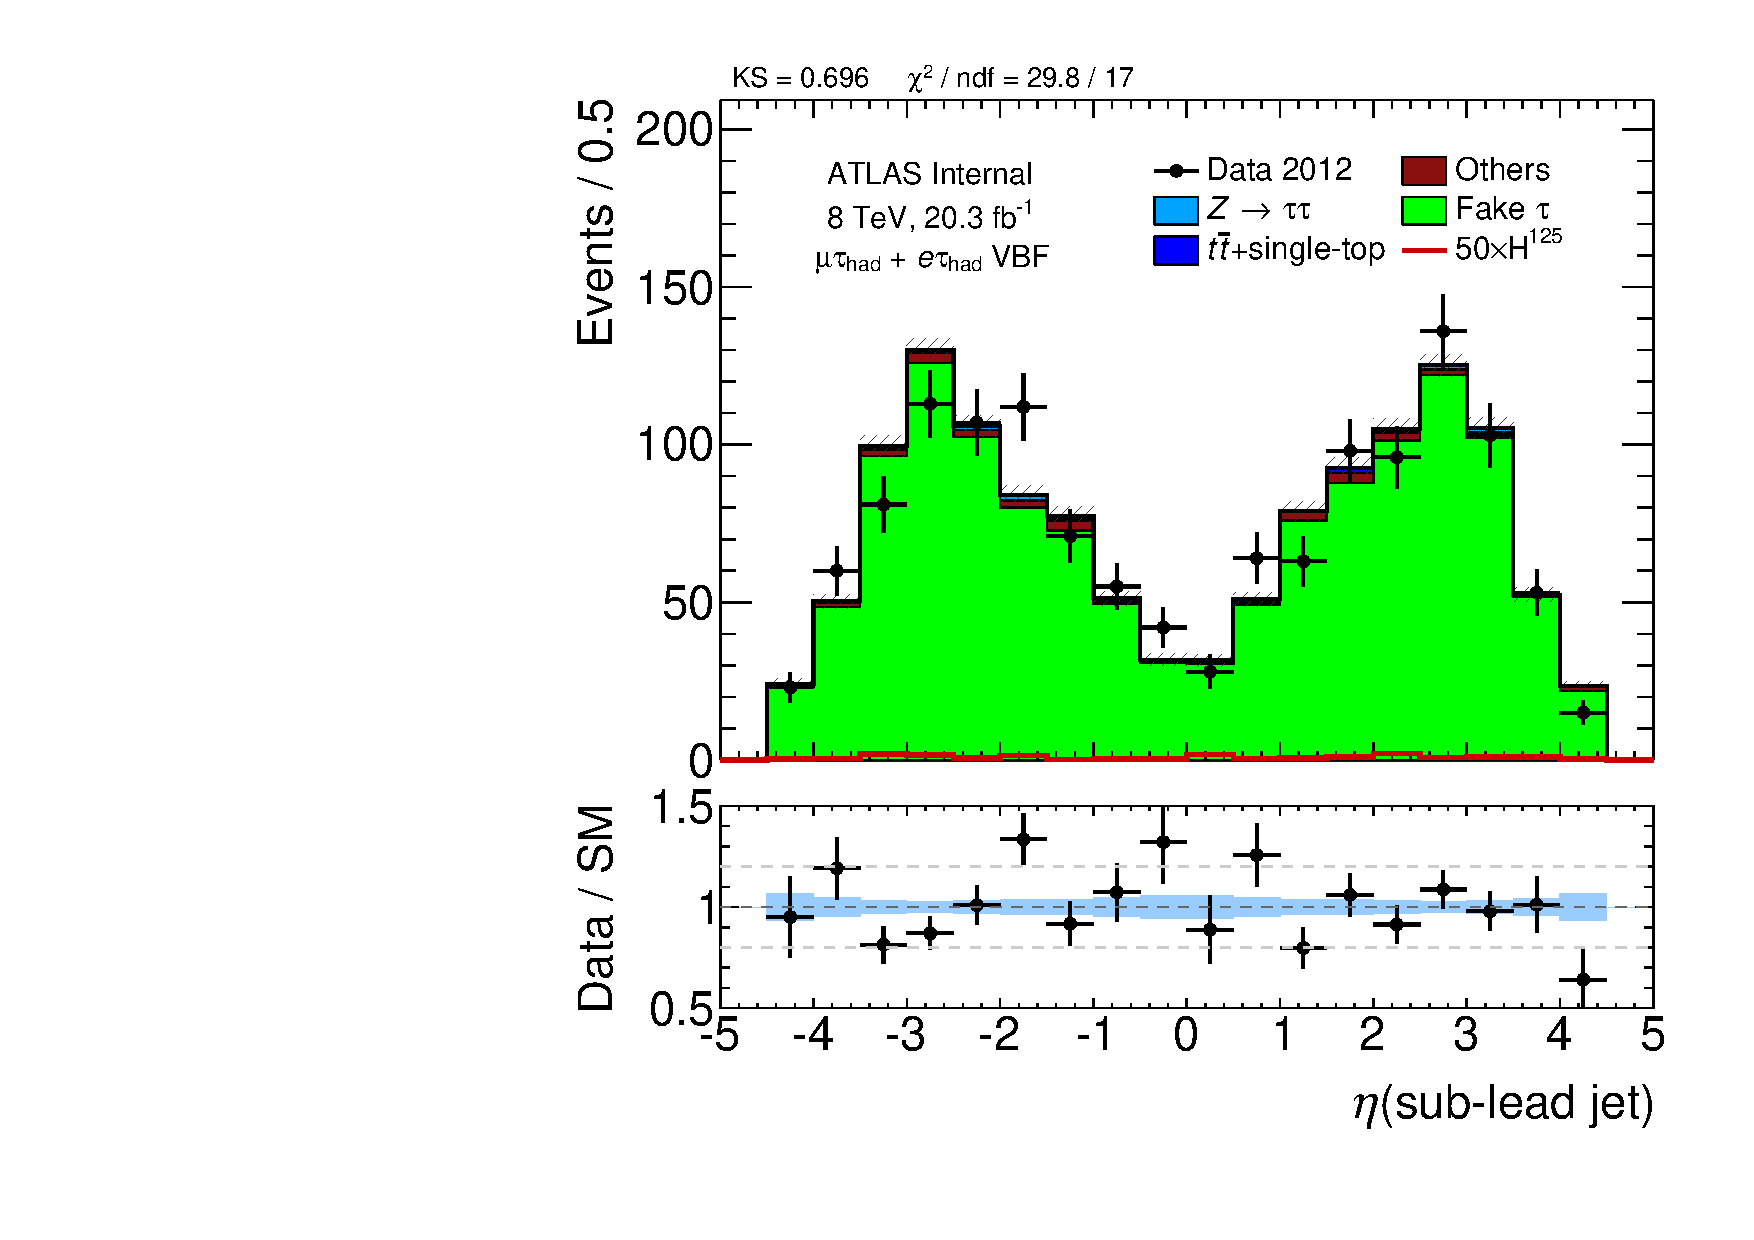
\includegraphics[width=0.32\textwidth]{figures/analysis/vbf-SSXCR/jet-2-eta}
  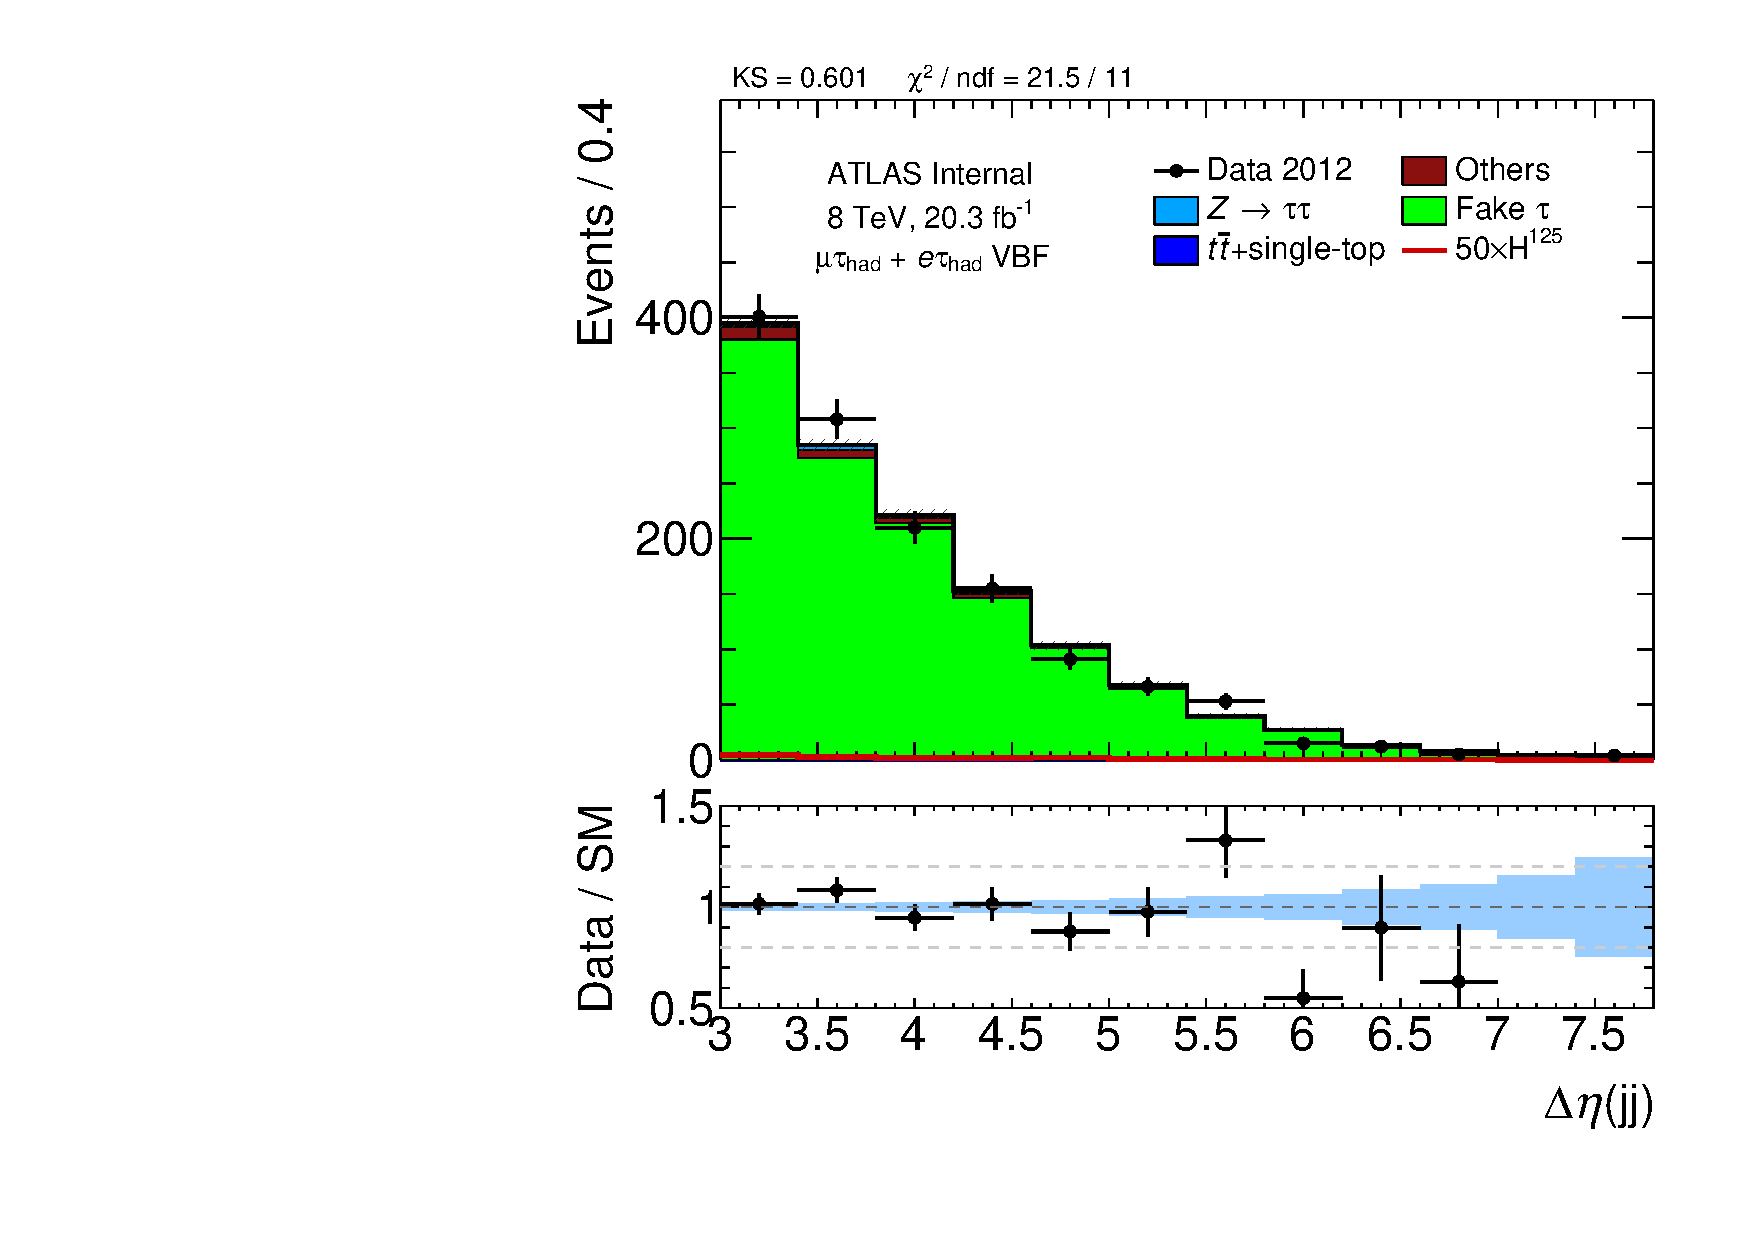
\includegraphics[width=0.32\textwidth]{figures/analysis/vbf-SSXCR/jets-deta}
  % --------------
  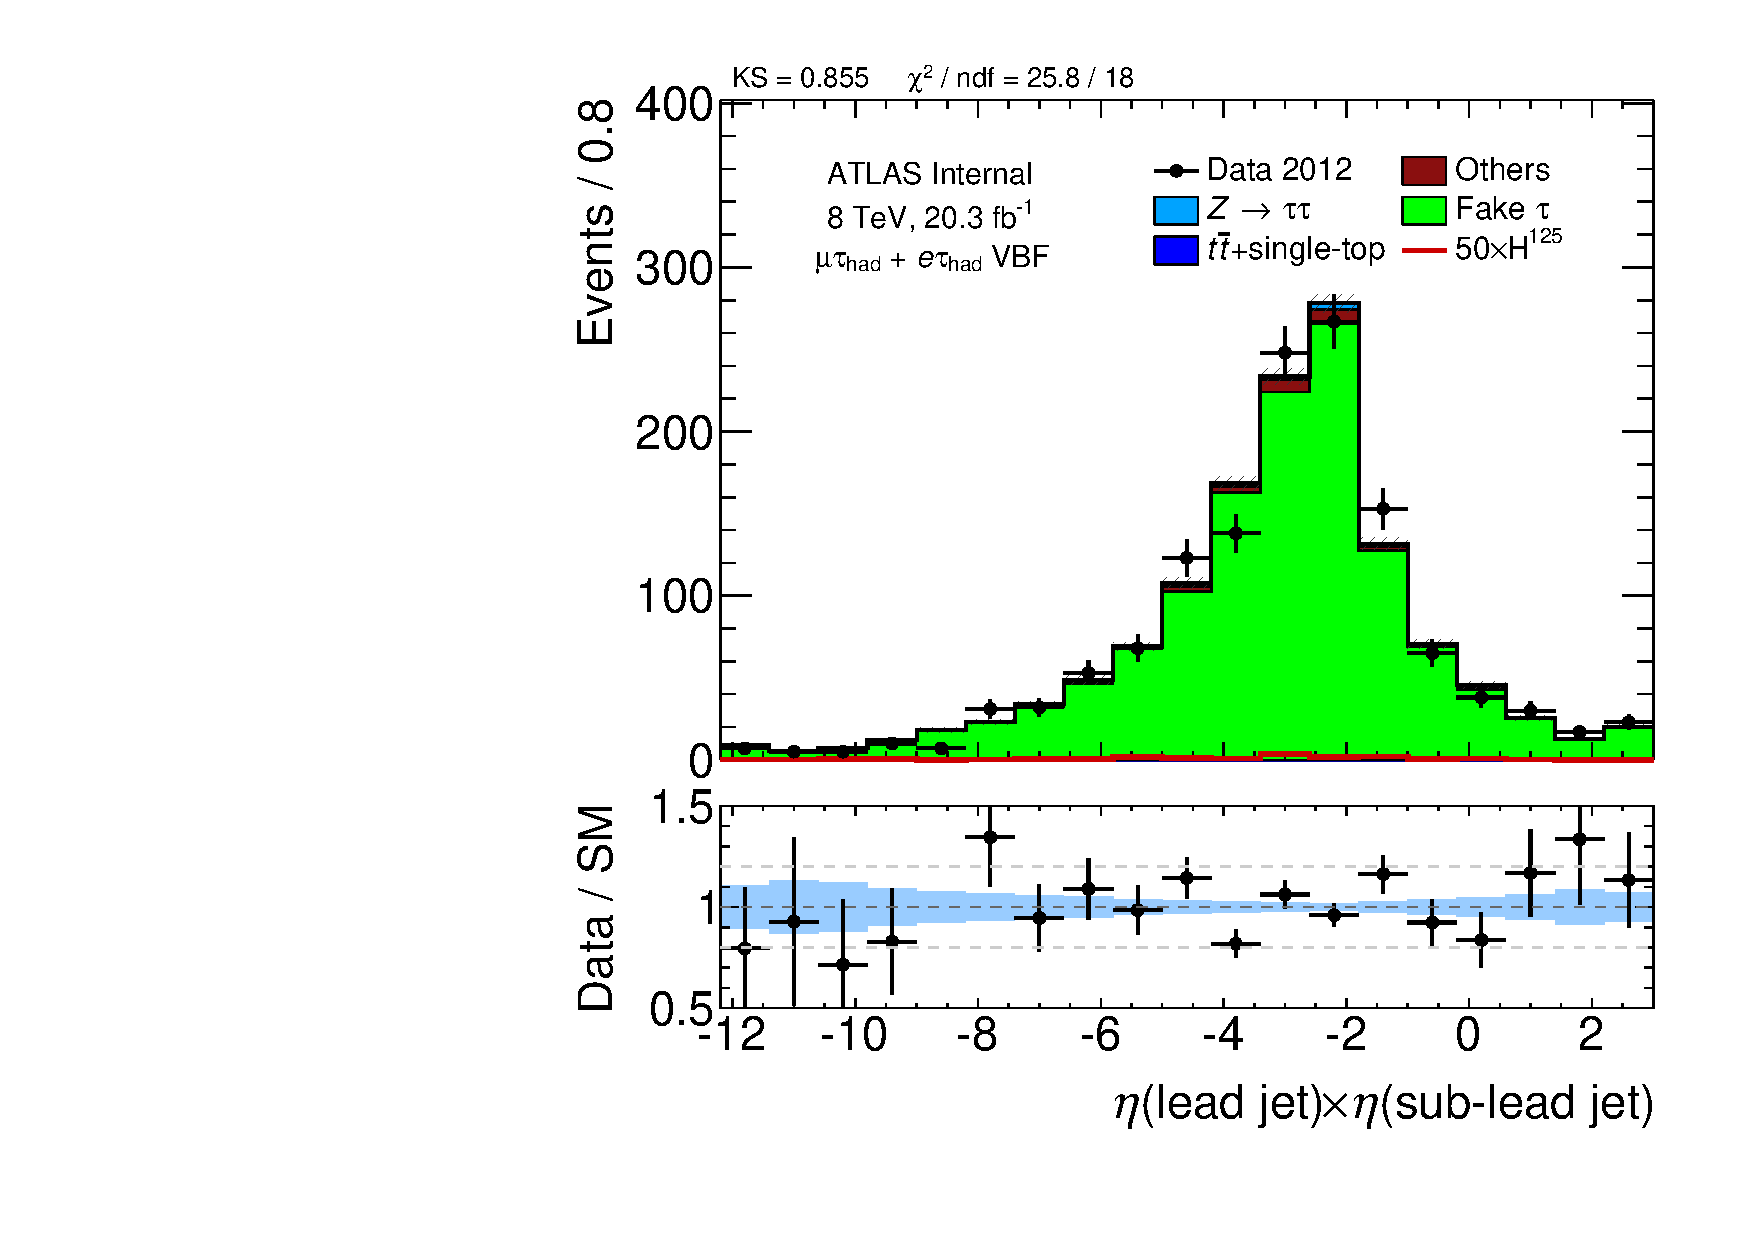
\includegraphics[width=0.32\textwidth]{figures/analysis/vbf-SSXCR/jets-etaprod}
  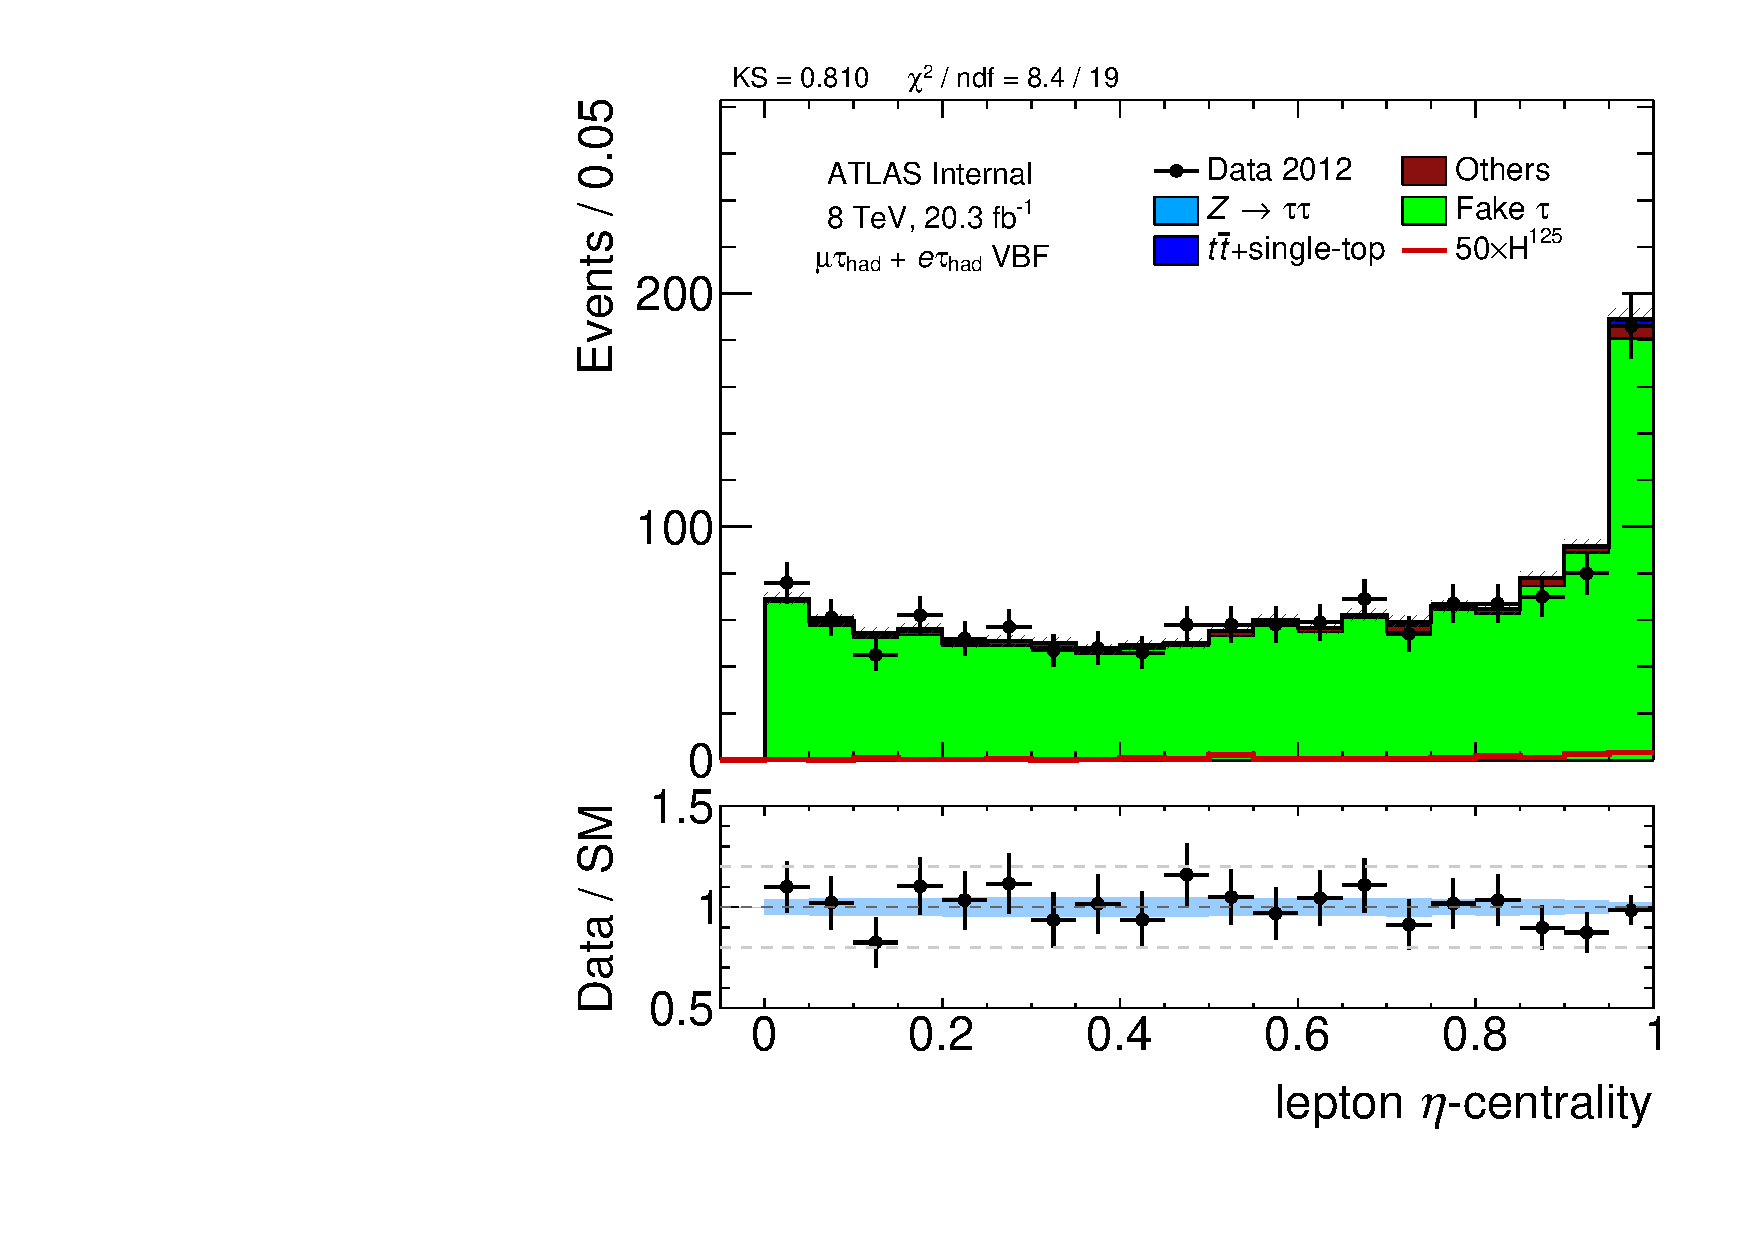
\includegraphics[width=0.32\textwidth]{figures/analysis/vbf-SSXCR/lep-eta-centrality}
  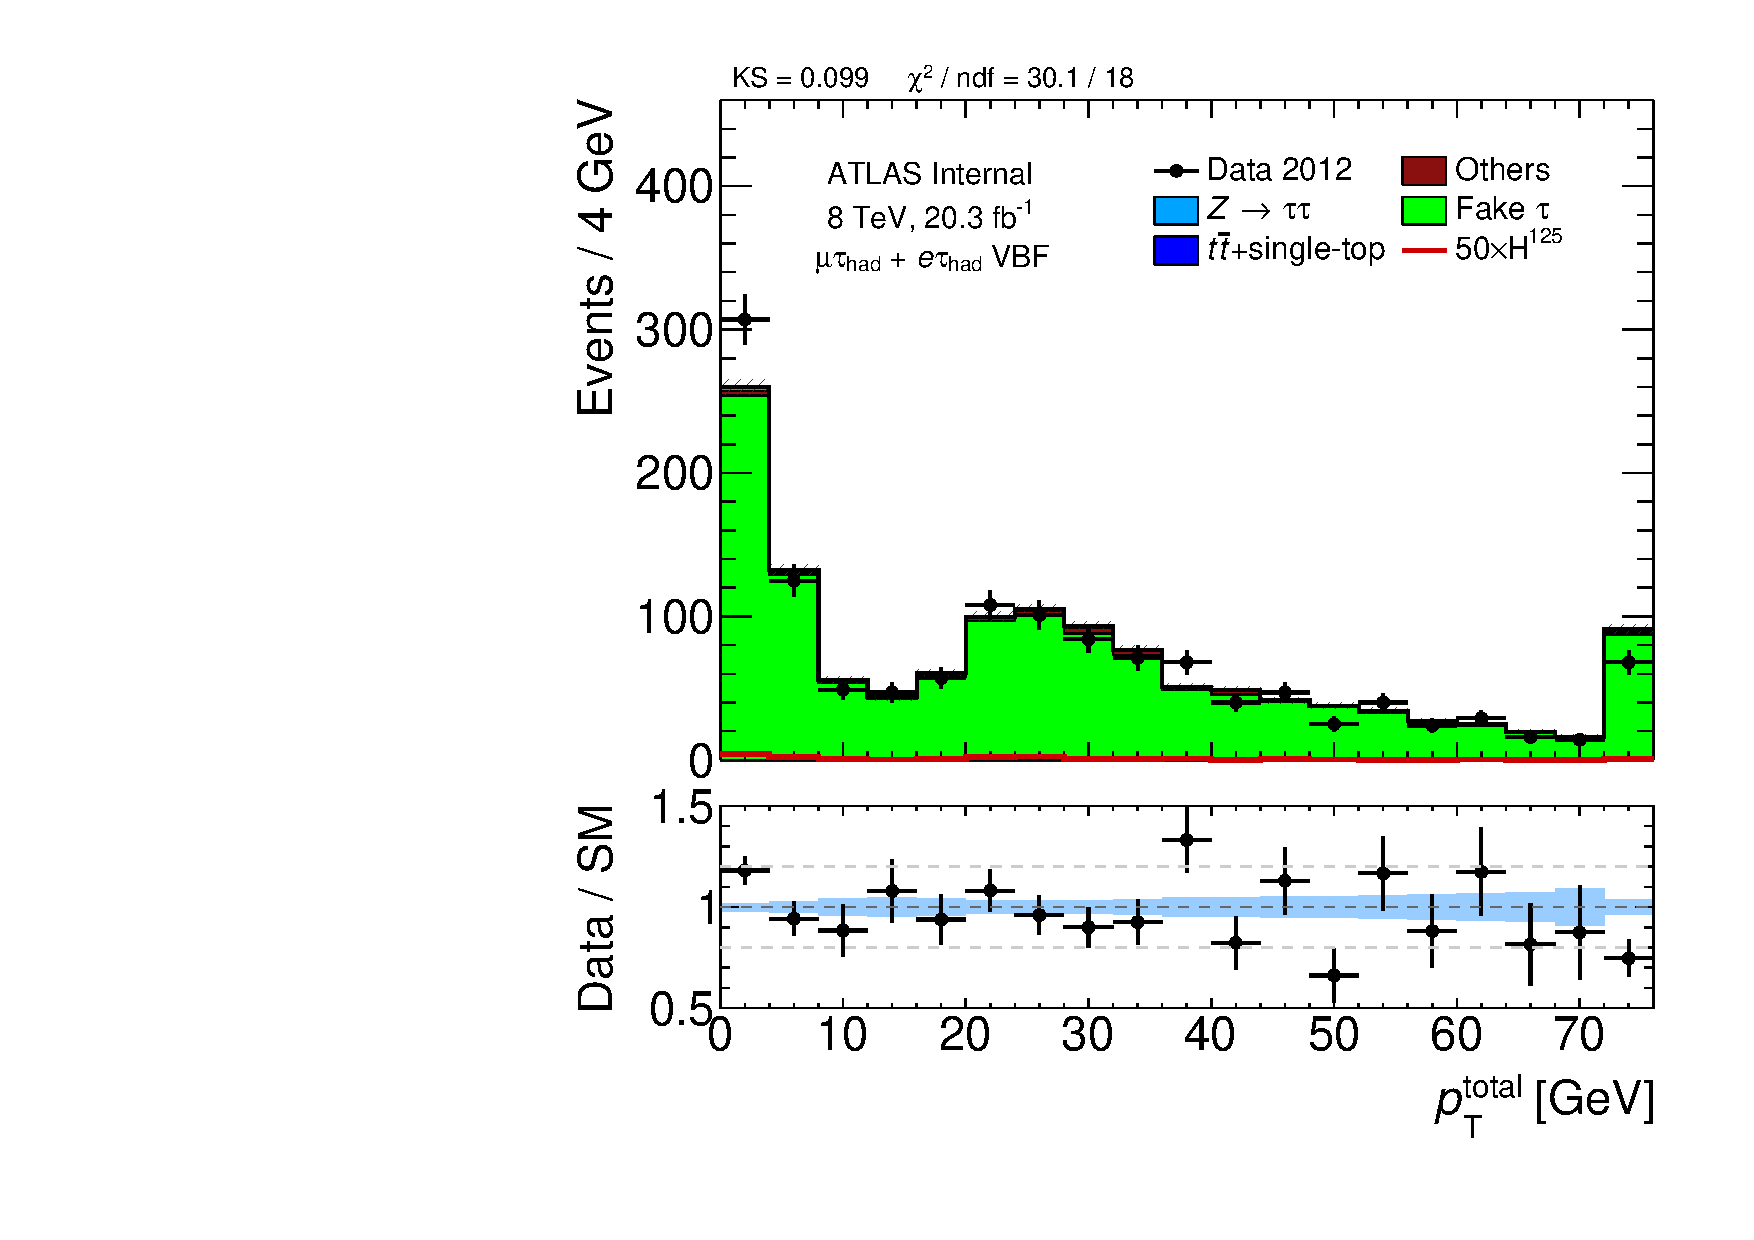
\includegraphics[width=0.32\textwidth]{figures/analysis/vbf-SSXCR/system-pt}
  % --------------
  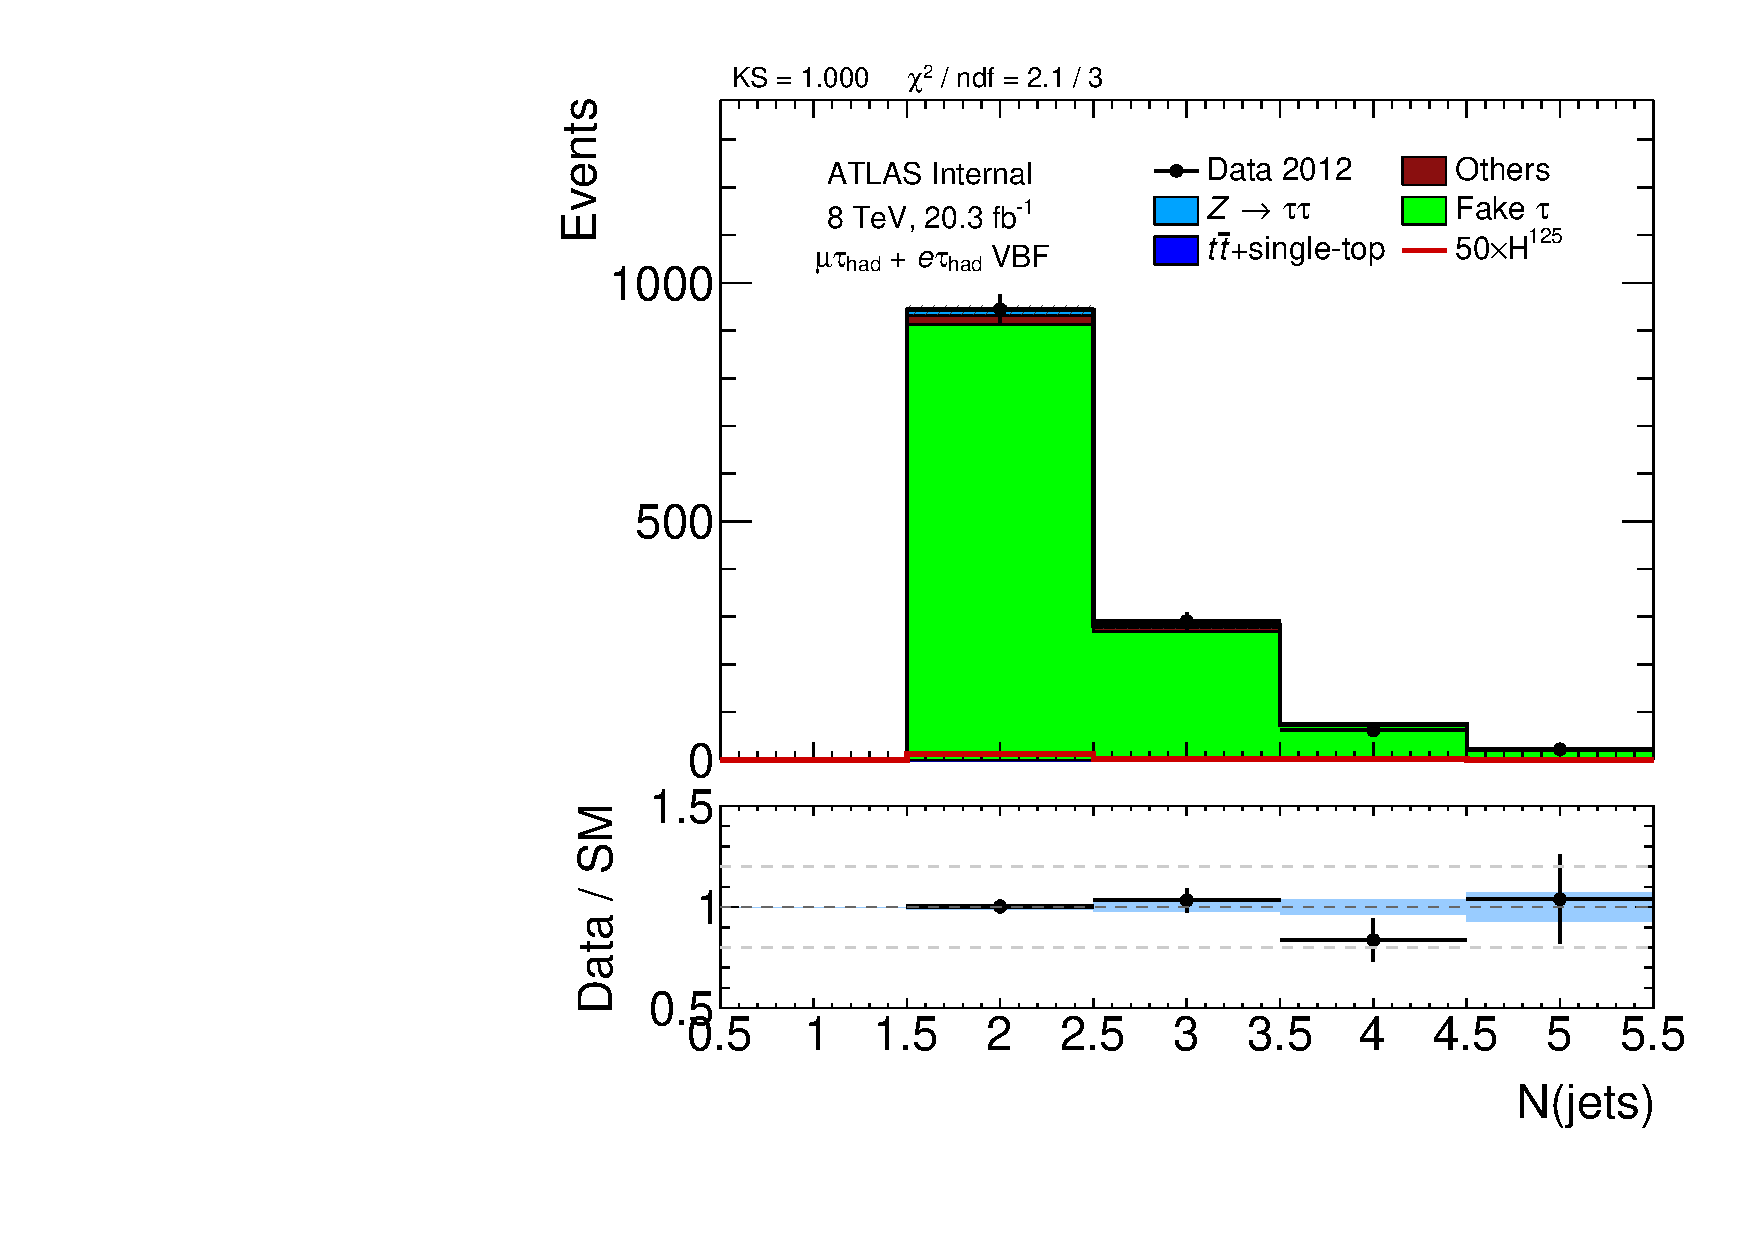
\includegraphics[width=0.32\textwidth]{figures/analysis/vbf-SSXCR/n-jets30}
  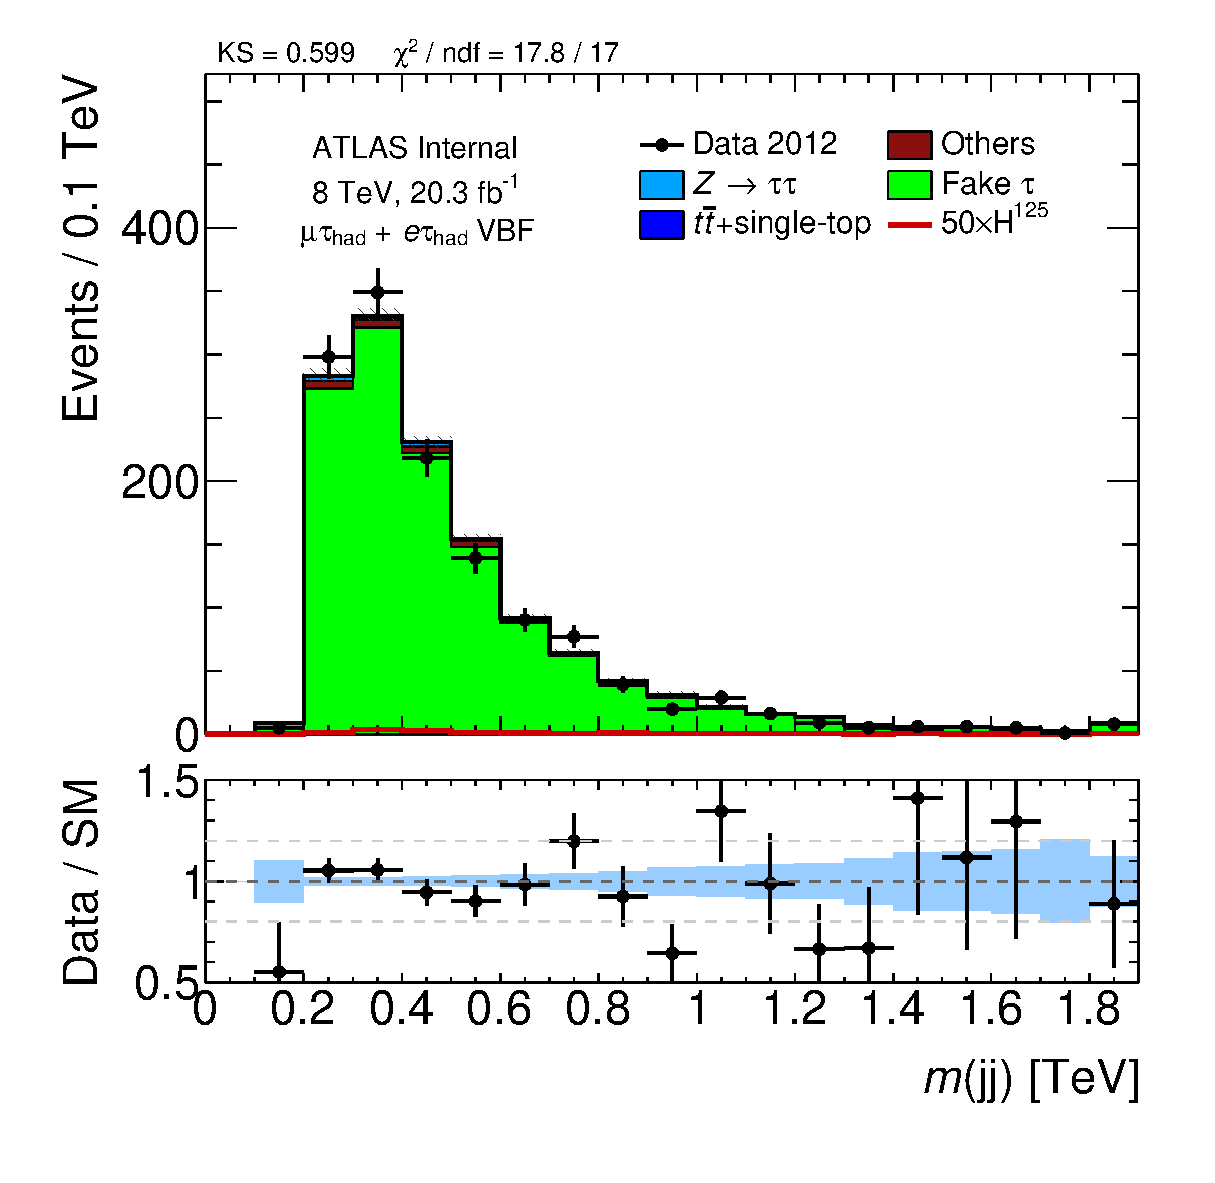
\includegraphics[width=0.32\textwidth]{figures/analysis/vbf-SSXCR/dijet-m-veryhigh}
  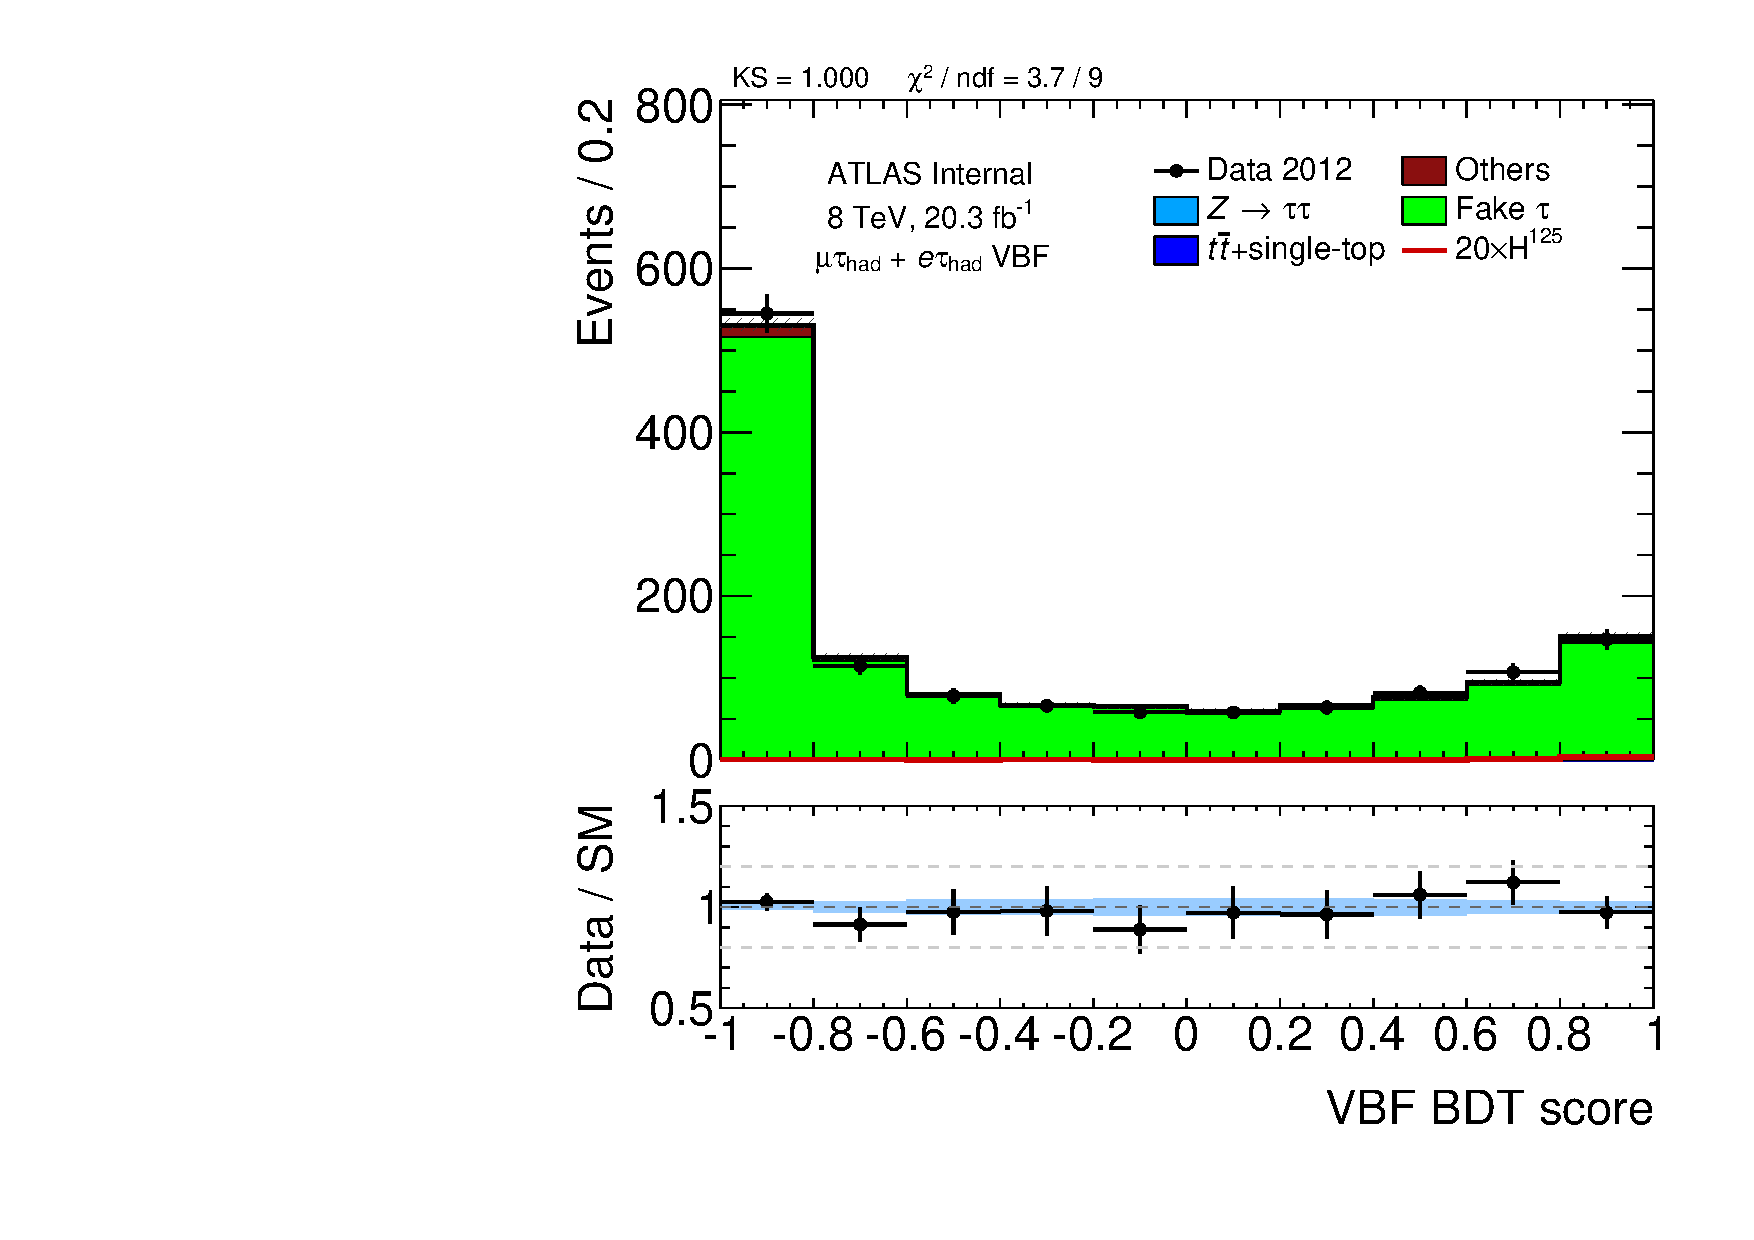
\includegraphics[width=0.32\textwidth]{figures/analysis/vbf-SSXCR/BDTEve-VBF}
  \caption{Variables.}
  \label{fig:backgrounds-SSXCR-jets}
\end{figure}

\clearpage
\begin{figure}[tp]
  \centering
  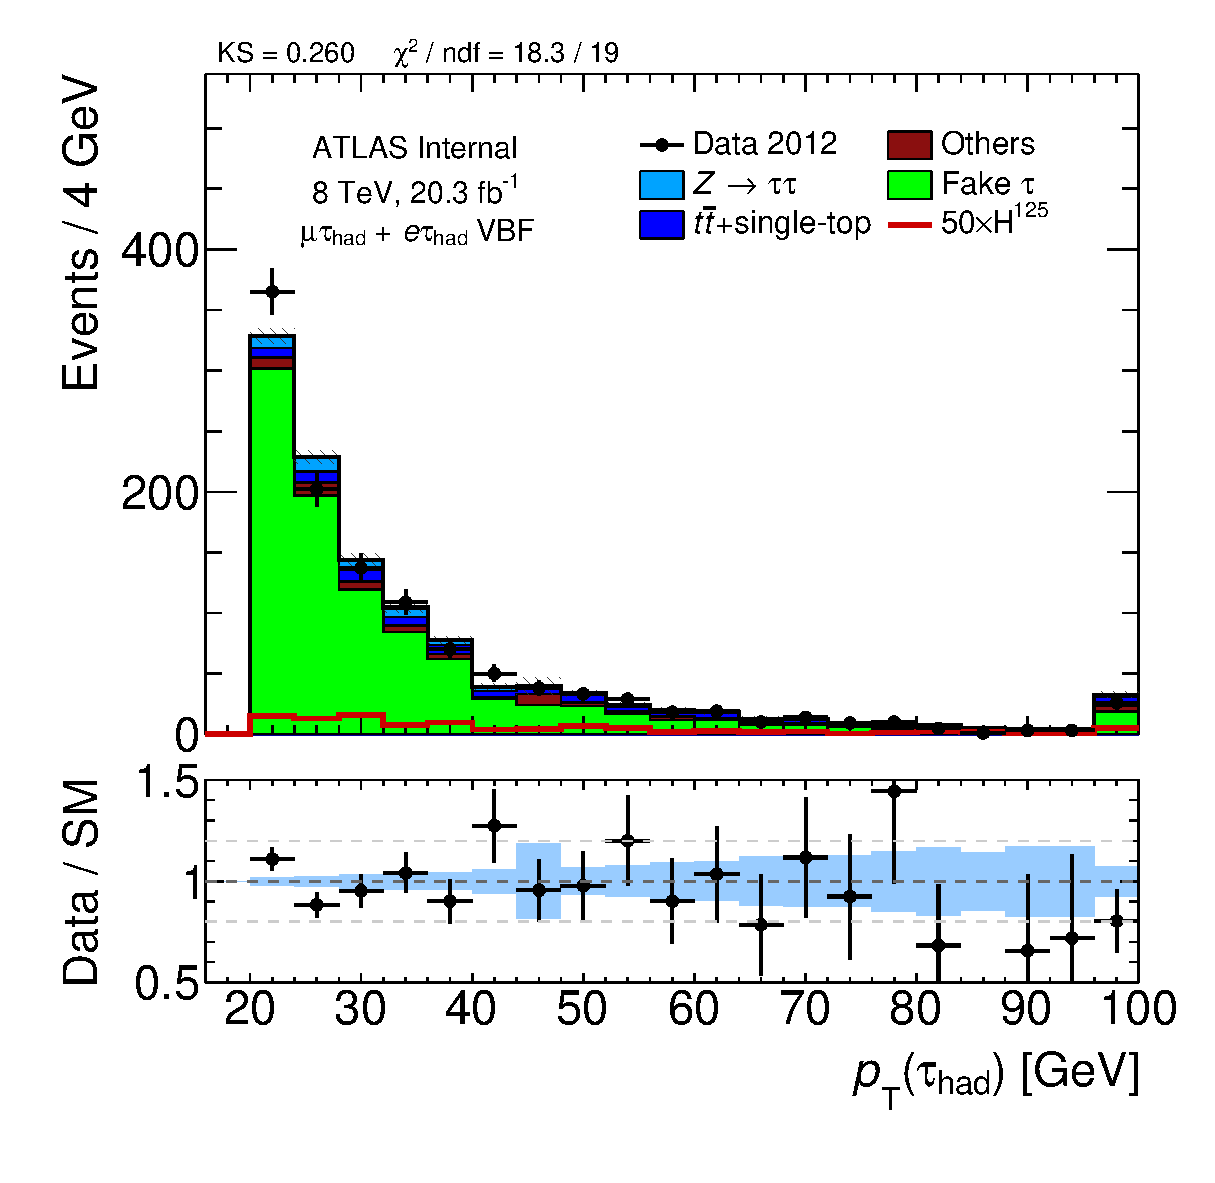
\includegraphics[width=0.32\textwidth]{figures/analysis/vbf-WlvCR/tau-pt}
  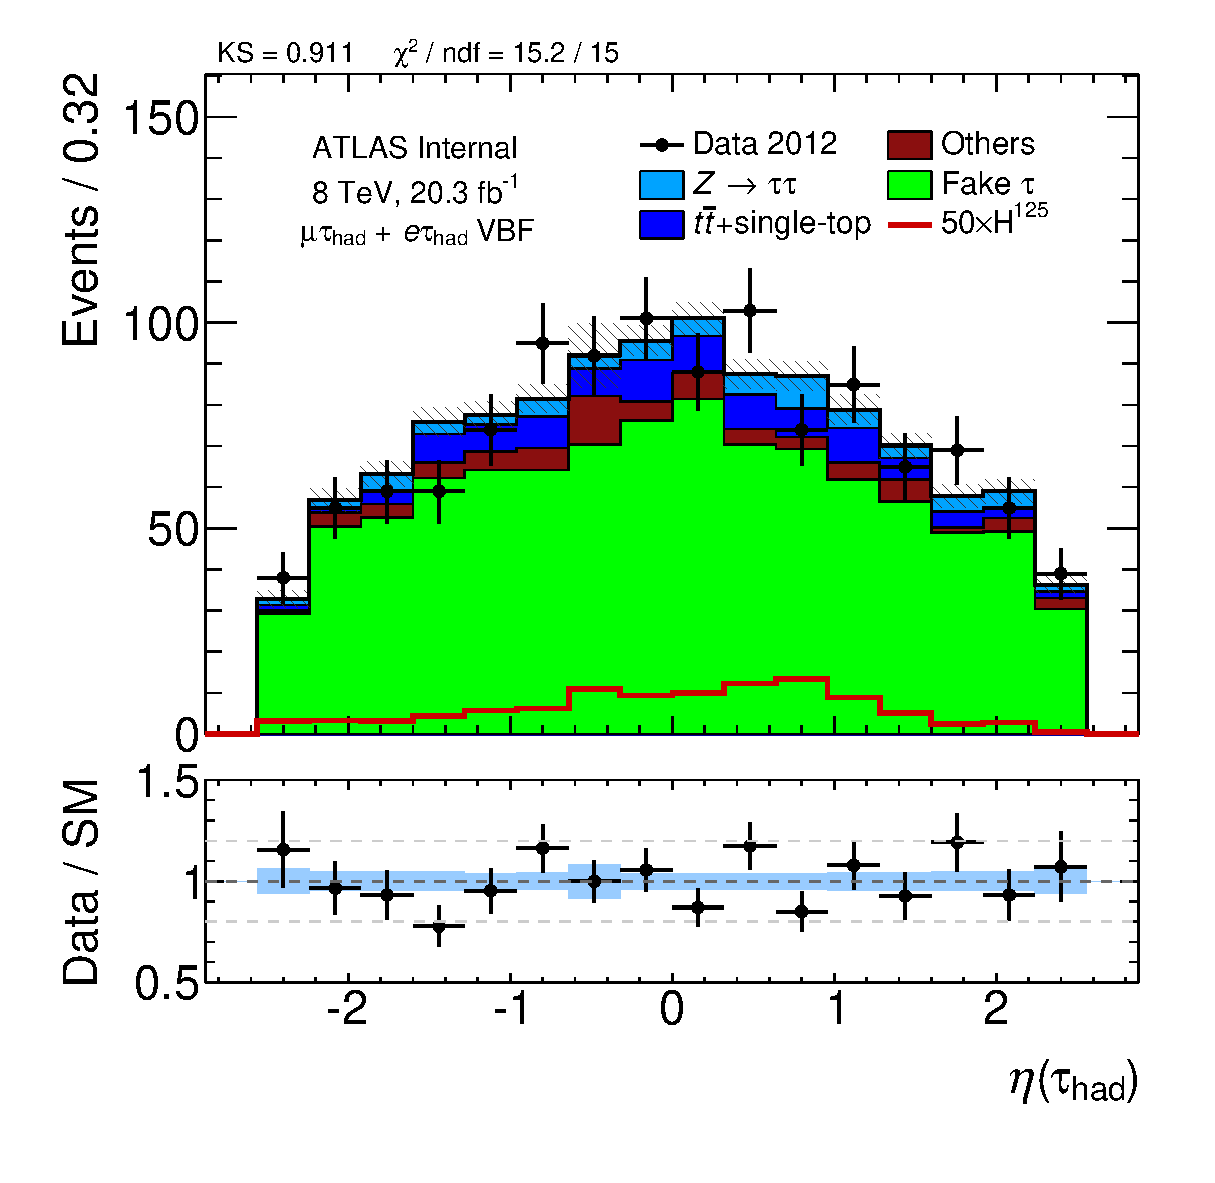
\includegraphics[width=0.32\textwidth]{figures/analysis/vbf-WlvCR/tau-eta}
  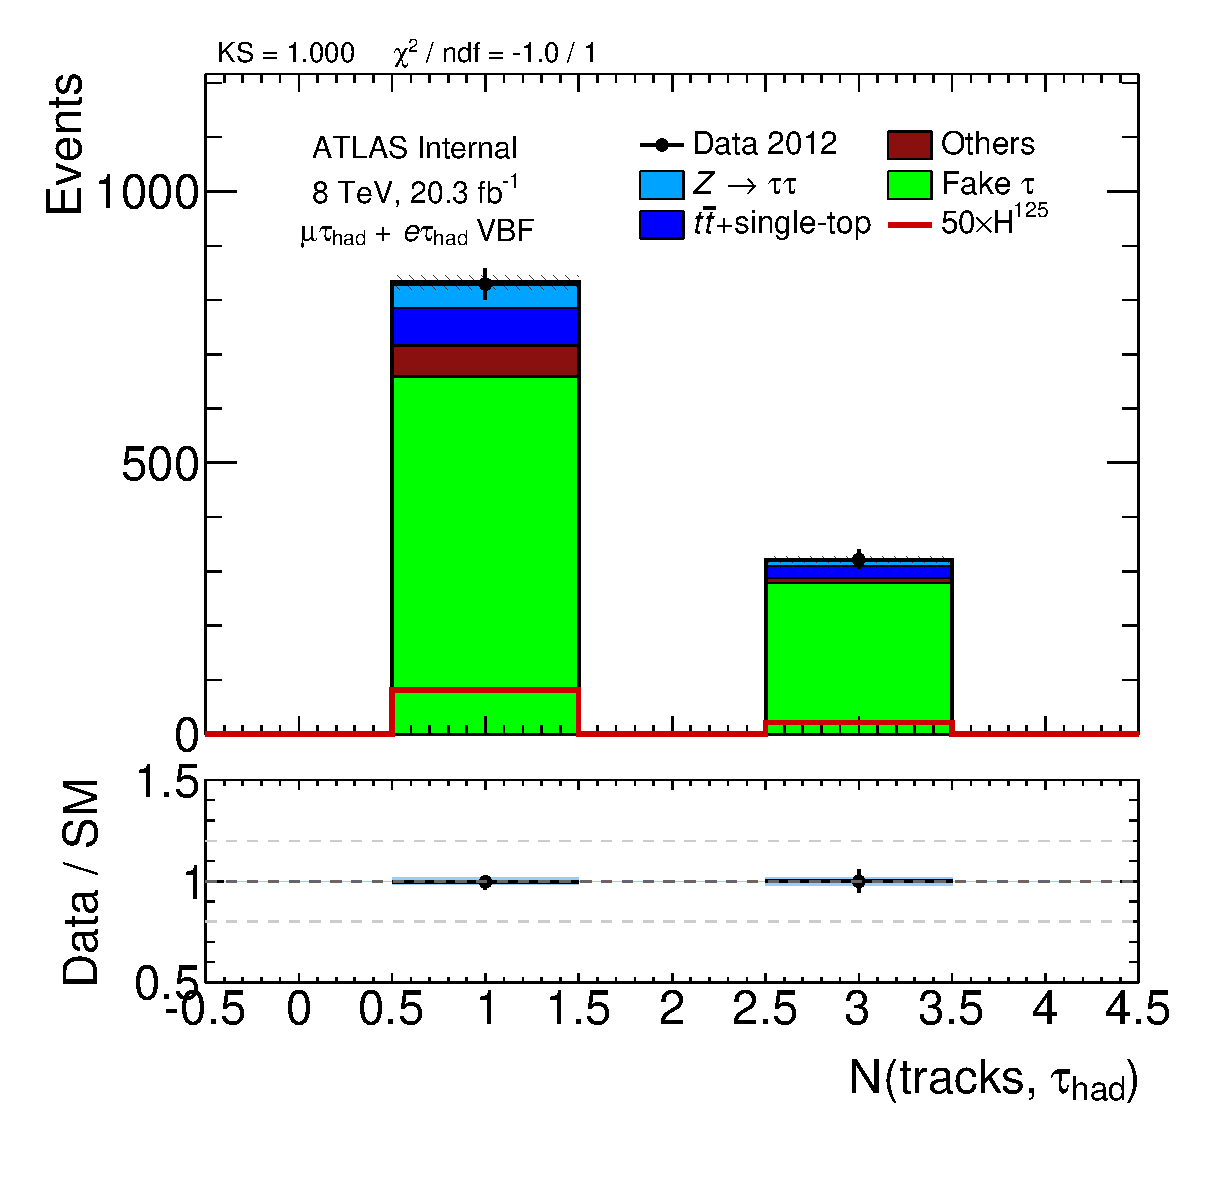
\includegraphics[width=0.32\textwidth]{figures/analysis/vbf-WlvCR/tau-numTrack}
  % --------------
  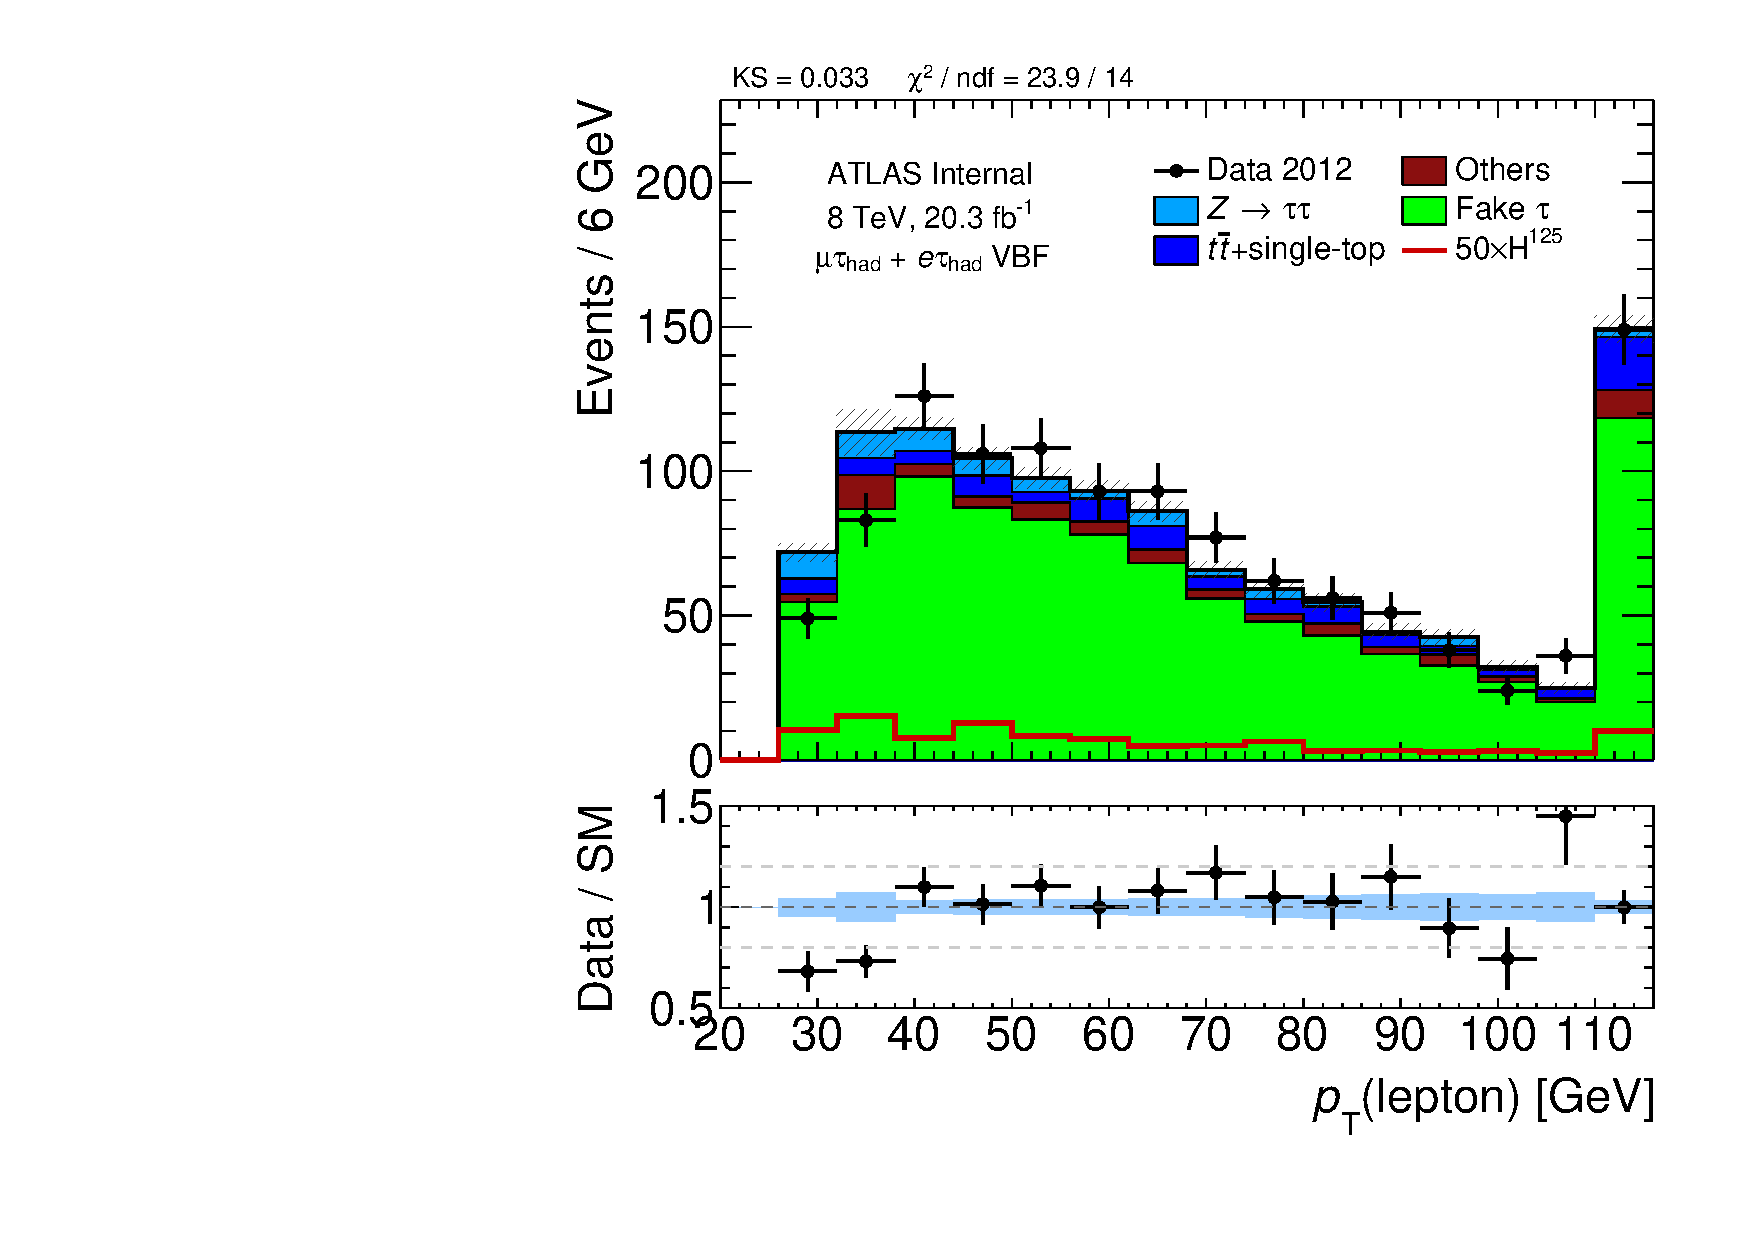
\includegraphics[width=0.32\textwidth]{figures/analysis/vbf-WlvCR/lep-pt-hi}
  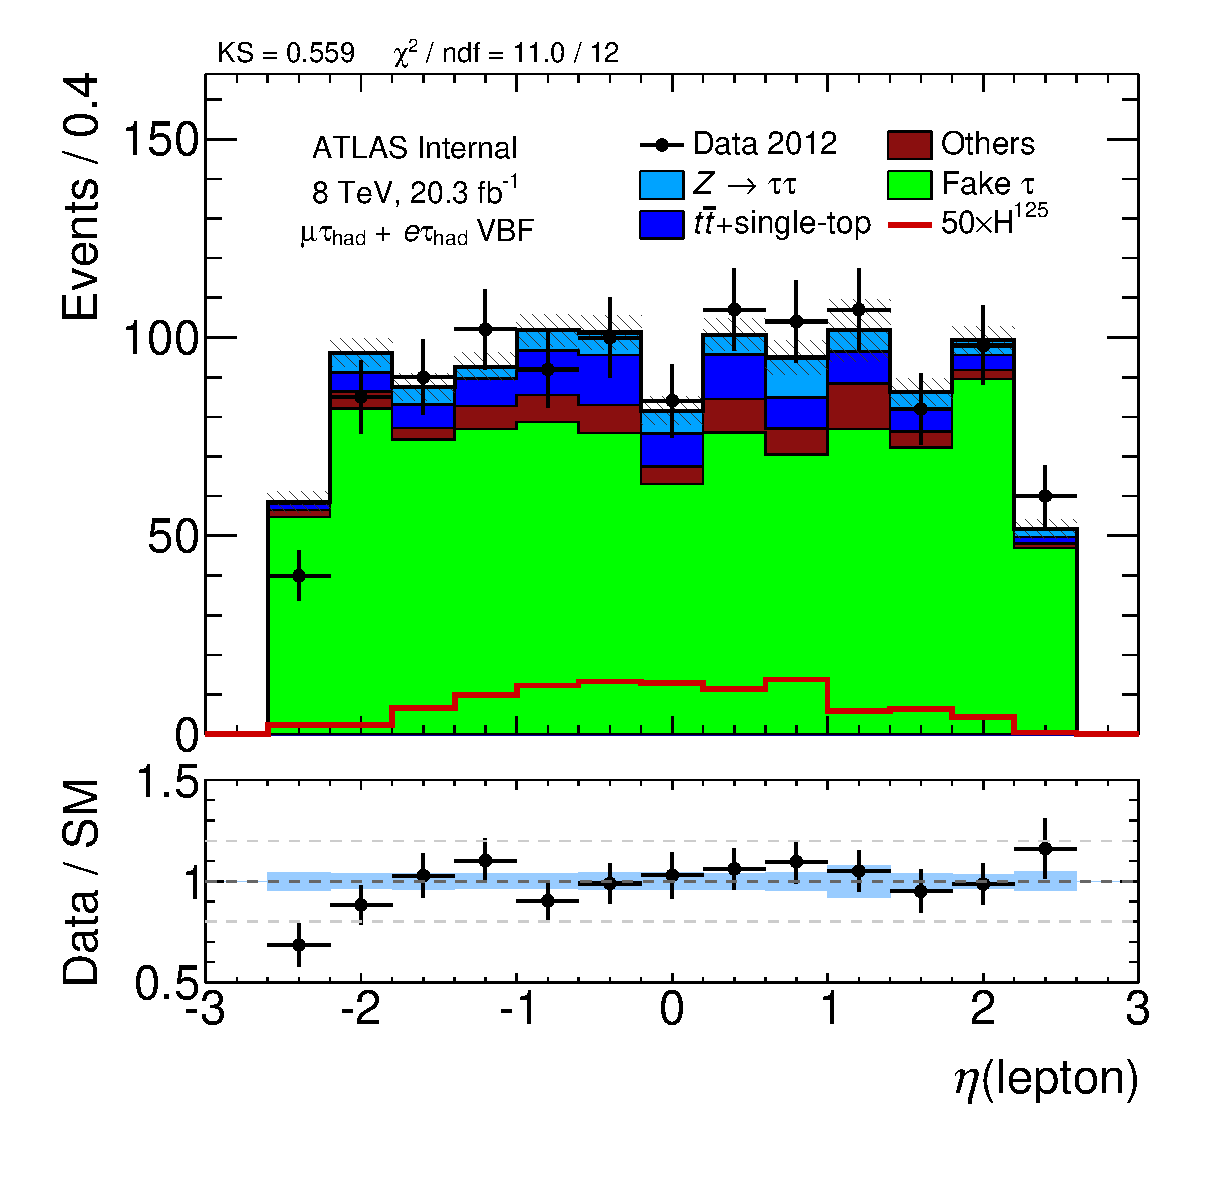
\includegraphics[width=0.32\textwidth]{figures/analysis/vbf-WlvCR/lep-eta}
  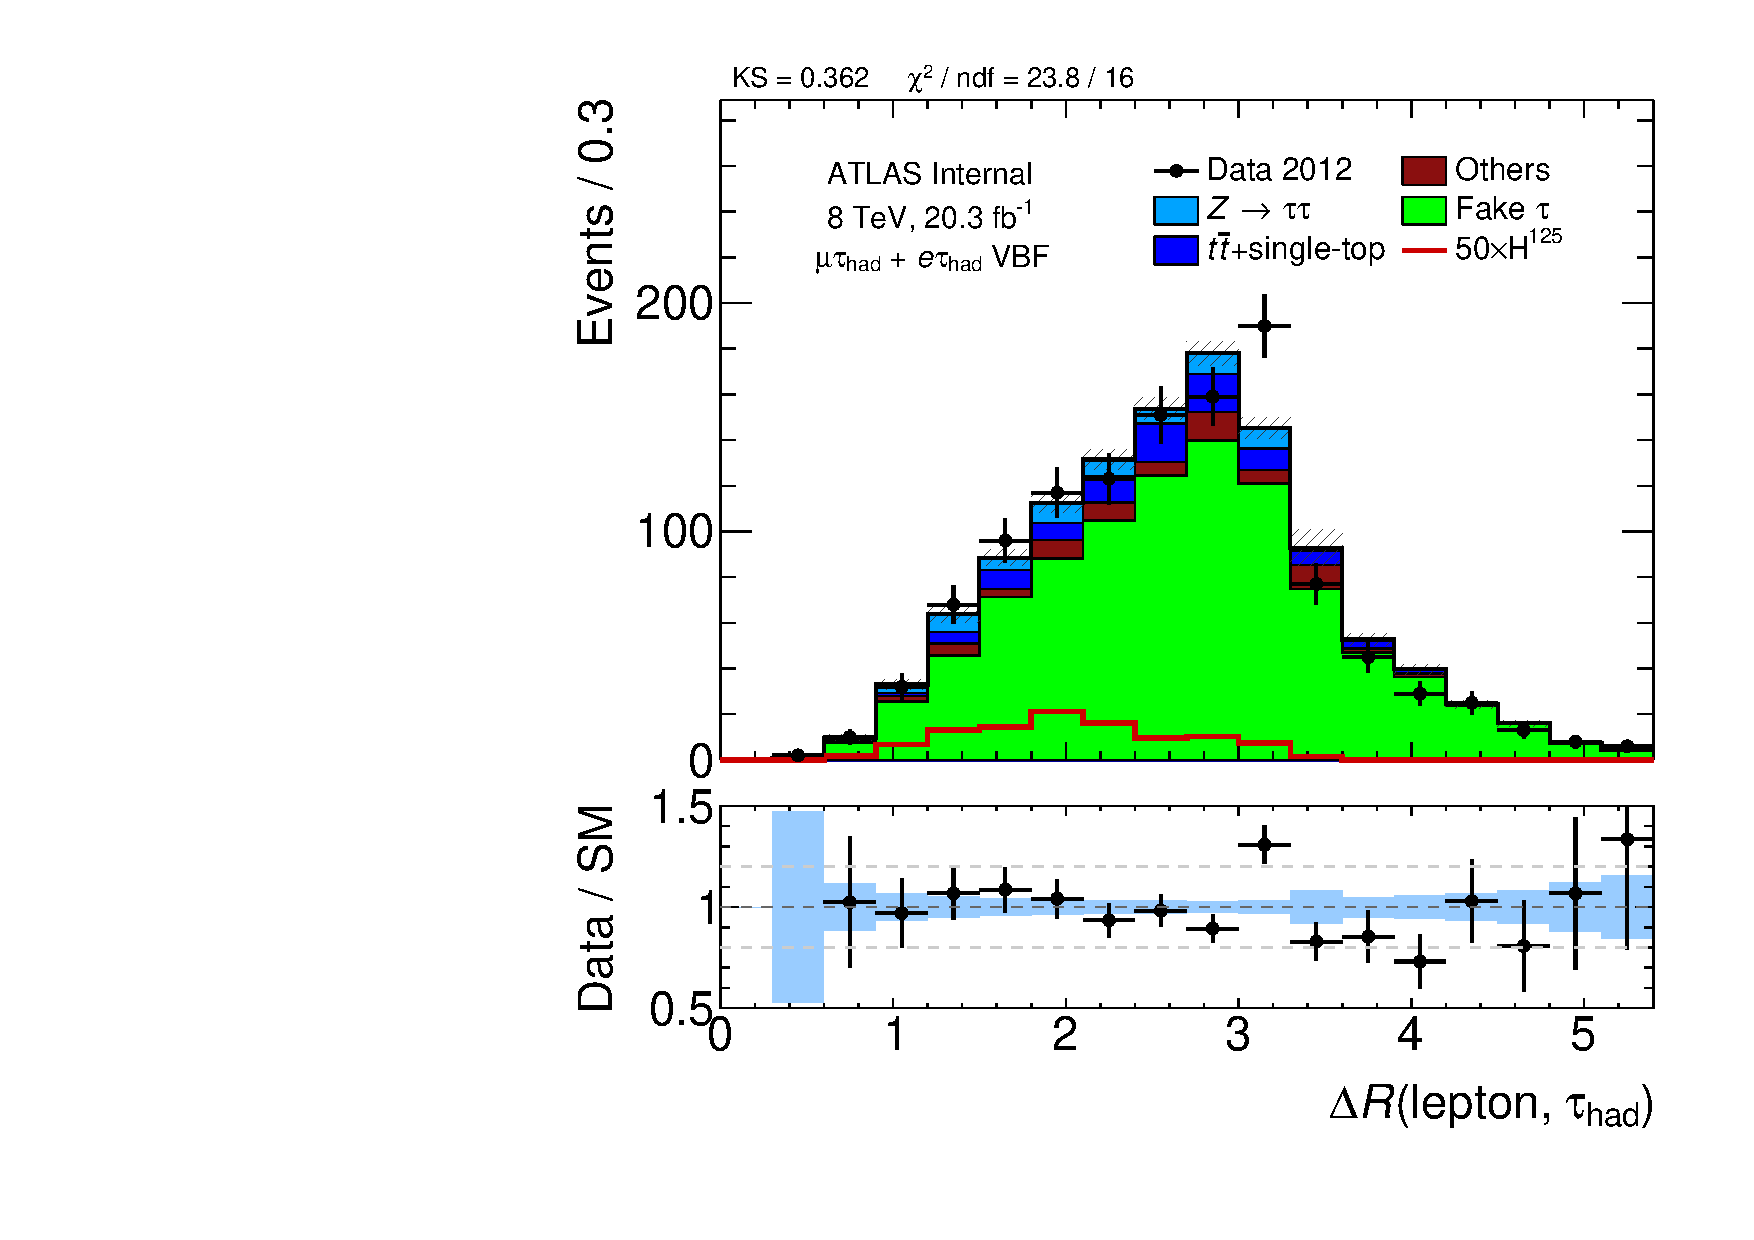
\includegraphics[width=0.32\textwidth]{figures/analysis/vbf-WlvCR/taulep-dR}
  % --------------
  \includegraphics[width=0.32\textwidth]{figures/analysis/vbf-WlvCR/met-pt-hi}
  \includegraphics[width=0.32\textwidth]{figures/analysis/vbf-WlvCR/mMMC}
  \includegraphics[width=0.32\textwidth]{figures/analysis/vbf-WlvCR/mT-hi}
  % --------------
  \includegraphics[width=0.32\textwidth]{figures/analysis/vbf-WlvCR/met-phi-centrality}
  \includegraphics[width=0.32\textwidth]{figures/analysis/vbf-WlvCR/H-pt-hi}
  \includegraphics[width=0.32\textwidth]{figures/analysis/vbf-WlvCR/mvis}
  \caption{Variables.}
  \label{fig:backgrounds-WlvCR-taus}
\end{figure}

\begin{figure}[tp]
  \includegraphics[width=0.32\textwidth]{figures/analysis/vbf-WlvCR/jet-1-pt}
  \includegraphics[width=0.32\textwidth]{figures/analysis/vbf-WlvCR/jet-1-eta}
  \includegraphics[width=0.32\textwidth]{figures/analysis/vbf-WlvCR/jets-dphi}
  % --------------
  \includegraphics[width=0.32\textwidth]{figures/analysis/vbf-WlvCR/jet-2-pt}
  \includegraphics[width=0.32\textwidth]{figures/analysis/vbf-WlvCR/jet-2-eta}
  \includegraphics[width=0.32\textwidth]{figures/analysis/vbf-WlvCR/jets-deta}
  % --------------
  \includegraphics[width=0.32\textwidth]{figures/analysis/vbf-WlvCR/jets-etaprod}
  \includegraphics[width=0.32\textwidth]{figures/analysis/vbf-WlvCR/lep-eta-centrality}
  \includegraphics[width=0.32\textwidth]{figures/analysis/vbf-WlvCR/system-pt}
  % --------------
  \includegraphics[width=0.32\textwidth]{figures/analysis/vbf-WlvCR/n-jets30}
  \includegraphics[width=0.32\textwidth]{figures/analysis/vbf-WlvCR/dijet-m-veryhigh}
  \includegraphics[width=0.32\textwidth]{figures/analysis/vbf-WlvCR/BDTEve-VBF}
  \caption{Variables.}
  \label{fig:backgrounds-WlvCR-jets}
\end{figure}

\clearpage
\begin{figure}[tp]
  \centering
  \includegraphics[width=0.32\textwidth]{figures/analysis/vbf-QCDCR/tau-pt}
  \includegraphics[width=0.32\textwidth]{figures/analysis/vbf-QCDCR/tau-eta}
  \includegraphics[width=0.32\textwidth]{figures/analysis/vbf-QCDCR/tau-numTrack}
  % --------------
  \includegraphics[width=0.32\textwidth]{figures/analysis/vbf-QCDCR/lep-pt-hi}
  \includegraphics[width=0.32\textwidth]{figures/analysis/vbf-QCDCR/lep-eta}
  \includegraphics[width=0.32\textwidth]{figures/analysis/vbf-QCDCR/taulep-dR}
  % --------------
  \includegraphics[width=0.32\textwidth]{figures/analysis/vbf-QCDCR/met-pt-hi}
  \includegraphics[width=0.32\textwidth]{figures/analysis/vbf-QCDCR/mMMC}
  \includegraphics[width=0.32\textwidth]{figures/analysis/vbf-QCDCR/mT}
  % --------------
  \includegraphics[width=0.32\textwidth]{figures/analysis/vbf-QCDCR/met-phi-centrality}
  \includegraphics[width=0.32\textwidth]{figures/analysis/vbf-QCDCR/H-pt-hi}
  \includegraphics[width=0.32\textwidth]{figures/analysis/vbf-QCDCR/mvis}
  \caption{Variables.}
  \label{fig:backgrounds-QCDCR-taus}
\end{figure}

\begin{figure}[tp]
  \includegraphics[width=0.32\textwidth]{figures/analysis/vbf-QCDCR/jet-1-pt}
  \includegraphics[width=0.32\textwidth]{figures/analysis/vbf-QCDCR/jet-1-eta}
  \includegraphics[width=0.32\textwidth]{figures/analysis/vbf-QCDCR/jets-dphi}
  % --------------
  \includegraphics[width=0.32\textwidth]{figures/analysis/vbf-QCDCR/jet-2-pt}
  \includegraphics[width=0.32\textwidth]{figures/analysis/vbf-QCDCR/jet-2-eta}
  \includegraphics[width=0.32\textwidth]{figures/analysis/vbf-QCDCR/jets-deta}
  % --------------
  \includegraphics[width=0.32\textwidth]{figures/analysis/vbf-QCDCR/jets-etaprod}
  \includegraphics[width=0.32\textwidth]{figures/analysis/vbf-QCDCR/lep-eta-centrality}
  \includegraphics[width=0.32\textwidth]{figures/analysis/vbf-QCDCR/system-pt}
  % --------------
  \includegraphics[width=0.32\textwidth]{figures/analysis/vbf-QCDCR/n-jets30}
  \includegraphics[width=0.32\textwidth]{figures/analysis/vbf-QCDCR/dijet-m-veryhigh}
  \includegraphics[width=0.32\textwidth]{figures/analysis/vbf-QCDCR/BDTEve-VBF}
  \caption{Variables.}
  \label{fig:backgrounds-QCDCR-jets}
\end{figure}

\clearpage
\begin{figure}[tp]
  \centering
  \includegraphics[width=0.32\textwidth]{figures/analysis/vbf-ZllCR/tau-pt}
  \includegraphics[width=0.32\textwidth]{figures/analysis/vbf-ZllCR/tau-eta}
  \includegraphics[width=0.32\textwidth]{figures/analysis/vbf-ZllCR/tau-numTrack}
  % --------------
  \includegraphics[width=0.32\textwidth]{figures/analysis/vbf-ZllCR/lep-pt-hi}
  \includegraphics[width=0.32\textwidth]{figures/analysis/vbf-ZllCR/lep-eta}
  \includegraphics[width=0.32\textwidth]{figures/analysis/vbf-ZllCR/taulep-dR}
  % --------------
  \includegraphics[width=0.32\textwidth]{figures/analysis/vbf-ZllCR/met-pt-hi}
  \includegraphics[width=0.32\textwidth]{figures/analysis/vbf-ZllCR/mMMC}
  \includegraphics[width=0.32\textwidth]{figures/analysis/vbf-ZllCR/mT}
  % --------------
  \includegraphics[width=0.32\textwidth]{figures/analysis/vbf-ZllCR/met-phi-centrality}
  \includegraphics[width=0.32\textwidth]{figures/analysis/vbf-ZllCR/H-pt-hi}
  \includegraphics[width=0.32\textwidth]{figures/analysis/vbf-ZllCR/mvis}
  \caption{Variables.}
  \label{fig:backgrounds-ZllCR-taus}
\end{figure}

\begin{figure}[tp]
  \includegraphics[width=0.32\textwidth]{figures/analysis/vbf-ZllCR/jet-1-pt}
  \includegraphics[width=0.32\textwidth]{figures/analysis/vbf-ZllCR/jet-1-eta}
  \includegraphics[width=0.32\textwidth]{figures/analysis/vbf-ZllCR/jets-dphi}
  % --------------
  \includegraphics[width=0.32\textwidth]{figures/analysis/vbf-ZllCR/jet-2-pt}
  \includegraphics[width=0.32\textwidth]{figures/analysis/vbf-ZllCR/jet-2-eta}
  \includegraphics[width=0.32\textwidth]{figures/analysis/vbf-ZllCR/jets-deta}
  % --------------
  \includegraphics[width=0.32\textwidth]{figures/analysis/vbf-ZllCR/jets-etaprod}
  \includegraphics[width=0.32\textwidth]{figures/analysis/vbf-ZllCR/lep-eta-centrality}
  \includegraphics[width=0.32\textwidth]{figures/analysis/vbf-ZllCR/system-pt}
  % --------------
  \includegraphics[width=0.32\textwidth]{figures/analysis/vbf-ZllCR/n-jets30}
  \includegraphics[width=0.32\textwidth]{figures/analysis/vbf-ZllCR/dijet-m-veryhigh}
  \includegraphics[width=0.32\textwidth]{figures/analysis/vbf-ZllCR/BDTEve-VBF}
  \caption{Variables.}
  \label{fig:backgrounds-ZllCR-jets}
\end{figure}

\clearpage
\begin{figure}[tp]
  \centering
  \includegraphics[width=0.32\textwidth]{figures/analysis/vbf-topCR/tau-pt}
  \includegraphics[width=0.32\textwidth]{figures/analysis/vbf-topCR/tau-eta}
  \includegraphics[width=0.32\textwidth]{figures/analysis/vbf-topCR/tau-numTrack}
  % --------------
  \includegraphics[width=0.32\textwidth]{figures/analysis/vbf-topCR/lep-pt-hi}
  \includegraphics[width=0.32\textwidth]{figures/analysis/vbf-topCR/lep-eta}
  \includegraphics[width=0.32\textwidth]{figures/analysis/vbf-topCR/taulep-dR}
  % --------------
  \includegraphics[width=0.32\textwidth]{figures/analysis/vbf-topCR/met-pt-hi}
  \includegraphics[width=0.32\textwidth]{figures/analysis/vbf-topCR/mMMC}
  \includegraphics[width=0.32\textwidth]{figures/analysis/vbf-topCR/mT}
  % --------------
  \includegraphics[width=0.32\textwidth]{figures/analysis/vbf-topCR/met-phi-centrality}
  \includegraphics[width=0.32\textwidth]{figures/analysis/vbf-topCR/H-pt-hi}
  \includegraphics[width=0.32\textwidth]{figures/analysis/vbf-topCR/mvis}
  \caption{Variables.}
  \label{fig:backgrounds-topCR-taus}
\end{figure}

\begin{figure}[tp]
  \includegraphics[width=0.32\textwidth]{figures/analysis/vbf-topCR/jet-1-pt}
  \includegraphics[width=0.32\textwidth]{figures/analysis/vbf-topCR/jet-1-eta}
  \includegraphics[width=0.32\textwidth]{figures/analysis/vbf-topCR/jets-dphi}
  % --------------
  \includegraphics[width=0.32\textwidth]{figures/analysis/vbf-topCR/jet-2-pt}
  \includegraphics[width=0.32\textwidth]{figures/analysis/vbf-topCR/jet-2-eta}
  \includegraphics[width=0.32\textwidth]{figures/analysis/vbf-topCR/jets-deta}
  % --------------
  \includegraphics[width=0.32\textwidth]{figures/analysis/vbf-topCR/jets-etaprod}
  \includegraphics[width=0.32\textwidth]{figures/analysis/vbf-topCR/lep-eta-centrality}
  \includegraphics[width=0.32\textwidth]{figures/analysis/vbf-topCR/system-pt}
  % --------------
  \includegraphics[width=0.32\textwidth]{figures/analysis/vbf-topCR/n-jets30}
  \includegraphics[width=0.32\textwidth]{figures/analysis/vbf-topCR/dijet-m-veryhigh}
  \includegraphics[width=0.32\textwidth]{figures/analysis/vbf-topCR/BDTEve-VBF}
  \caption{Variables.}
  \label{fig:backgrounds-topCR-jets}
\end{figure}

\clearpage
\begin{figure}[tp]
  \centering
  \includegraphics[width=0.32\textwidth]{figures/analysis/vbf-MCXSR/tau-pt}
  \includegraphics[width=0.32\textwidth]{figures/analysis/vbf-MCXSR/tau-eta}
  \includegraphics[width=0.32\textwidth]{figures/analysis/vbf-MCXSR/tau-numTrack}
  % --------------
  \includegraphics[width=0.32\textwidth]{figures/analysis/vbf-MCXSR/lep-pt-hi}
  \includegraphics[width=0.32\textwidth]{figures/analysis/vbf-MCXSR/lep-eta}
  \includegraphics[width=0.32\textwidth]{figures/analysis/vbf-MCXSR/taulep-dR}
  % --------------
  \includegraphics[width=0.32\textwidth]{figures/analysis/vbf-MCXSR/met-pt-hi}
  \includegraphics[width=0.32\textwidth]{figures/analysis/vbf-MCXSR/mMMC}
  \includegraphics[width=0.32\textwidth]{figures/analysis/vbf-MCXSR/mT}
  % --------------
  \includegraphics[width=0.32\textwidth]{figures/analysis/vbf-MCXSR/met-phi-centrality}
  \includegraphics[width=0.32\textwidth]{figures/analysis/vbf-MCXSR/H-pt-hi}
  \includegraphics[width=0.32\textwidth]{figures/analysis/vbf-MCXSR/mvis}
  \caption{Variables.}
  \label{fig:backgrounds-MCXSR-taus}
\end{figure}

\begin{figure}[tp]
  \includegraphics[width=0.32\textwidth]{figures/analysis/vbf-MCXSR/jet-1-pt}
  \includegraphics[width=0.32\textwidth]{figures/analysis/vbf-MCXSR/jet-1-eta}
  \includegraphics[width=0.32\textwidth]{figures/analysis/vbf-MCXSR/jets-dphi}
  % --------------
  \includegraphics[width=0.32\textwidth]{figures/analysis/vbf-MCXSR/jet-2-pt}
  \includegraphics[width=0.32\textwidth]{figures/analysis/vbf-MCXSR/jet-2-eta}
  \includegraphics[width=0.32\textwidth]{figures/analysis/vbf-MCXSR/jets-deta}
  % --------------
  \includegraphics[width=0.32\textwidth]{figures/analysis/vbf-MCXSR/jets-etaprod}
  \includegraphics[width=0.32\textwidth]{figures/analysis/vbf-MCXSR/lep-eta-centrality}
  \includegraphics[width=0.32\textwidth]{figures/analysis/vbf-MCXSR/system-pt}
  % --------------
  \includegraphics[width=0.32\textwidth]{figures/analysis/vbf-MCXSR/n-jets30}
  \includegraphics[width=0.32\textwidth]{figures/analysis/vbf-MCXSR/dijet-m-high}
  \includegraphics[width=0.32\textwidth]{figures/analysis/vbf-MCXSR/BDTEve-VBF}
  \caption{Variables.}
  \label{fig:backgrounds-MCXSR-jets}
\end{figure}


